%% Package and Class "uiucthesis2014" for use with LaTeX2e.
\documentclass[edeposit,fullpage]{uiucthesis2018}


\usepackage[acronym,toc]{glossaries}
\usepackage{listings}
\usepackage{minted}
\usepackage{appendix}

\usepackage{xspace}
\usepackage{graphics}

\newcommand{\Cycamore}{\textsc{Cycamore}\xspace}
\newcommand{\Cyclus}{\textsc{Cyclus}\xspace}
\newcommand{\SaltProc}{\textsc{SaltProc}\xspace}
\newcommand{\OpenMC}{\textsc{OpenMC}\xspace}
\newcommand{\SerpentTWO}{\textsc{Serpent2}\xspace}
\newcommand{\ONIX}{\textsc{ONIX}\xspace}
\newcommand{\NJOYTWOONE}{\textsc{NJOY21}\xspace}
\newcommand{\ChemTriton}{\textsc{ChemTriton}\xspace}
\newcommand{\Shift}{\textsc{Shift}\xspace}
\newcommand{\SCALE}{\textsc{SCALE}\xspace}
\newcommand{\TRITON}{\textsc{TRITON}\xspace}
\newcommand{\ORIGEN}{\textsc{ORIGEN}\xspace}
\newcommand{\MCNPSIX}{\textsc{MCNP6}\xspace}
\newcommand{\CINDERNINETY}{\textsc{CINDER90}\xspace}
\newcommand{\ADDER}{\textsc{ADDER}\xspace}

\usepackage{placeins}
\usepackage{booktabs} % nice rules (thick lines) for tables
\usepackage{microtype} % improves typography for PDF

\usepackage[hyphens]{url}
\usepackage{hyperref}
\usepackage{subfig}
\usepackage{hhline}
\usepackage{amsmath}
\usepackage{color}
\usepackage{multirow}
\usepackage{siunitx} % typesetting for units
\usepackage{tabulary}
\usepackage[version=4]{mhchem}
\sisetup{
    input-decimal-markers = .,input-ignore = {,},table-number-alignment = right,
    group-separator={,}, group-four-digits = true
}
\usepackage{booktabs}
\newcommand\tab[1][1cm]{\hspace*{#1}}

\usepackage{threeparttable, tablefootnote}

%tikzpicture fit to page width
\usepackage{environ}
\makeatletter
\newsavebox{\measure@tikzpicture}
\NewEnviron{scaletikzpicturetowidth}[1]{%
  \def\tikz@width{#1}%
  \def\tikzscale{1}\begin{lrbox}{\measure@tikzpicture}%
  \BODY
  \end{lrbox}
  \pgfmathparse{#1/\wd\measure@tikzpicture}%
  \edef\tikzscale{\pgfmathresult}%
  \BODY
}

\usepackage{tabularx}
\newcolumntype{b}{>{\hsize=1.0\hsize}X}
\newcolumntype{q}{>{\hsize=0.5\hsize}X}
\newcolumntype{R}{>{\raggedleft\arraybackslash\hsize=0.5\hsize}X}
\newcolumntype{z}{>{\hsize=0.75\hsize}X}
\newcolumntype{s}{>{\hsize=.5\hsize}X}
\newcolumntype{m}{>{\hsize=.75\hsize}X}

\usepackage{cleveref}
\usepackage{datatool}
\usepackage[numbers]{natbib}
\usepackage{notoccite}


\usepackage{tikz}
\usetikzlibrary{positioning, arrows, decorations, shapes}

\usetikzlibrary{shapes.geometric,arrows}
\tikzstyle{process} = [rectangle, rounded corners, minimum width=2.5cm, minimum height=1cm,text centered, draw=black, fill=blue!30]

\tikzstyle{object} = [ellipse, rounded corners, minimum width=3cm, minimum height=1cm,text centered, draw=black, fill=green!30]
\tikzstyle{objectr} = [ellipse, rounded corners, minimum width=3cm, minimum height=1cm,text centered, draw=black, fill=red!30]

\tikzstyle{empty} =  [rectangle, rounded corners, minimum width=2.5cm, minimum height=0.7cm,text centered, draw=black, fill=white!30]
\tikzstyle{arrow} = [thick,->,>=stealth]


\title{Implementation and validation of \OpenMC in \SaltProc}
\author{Oleksandr Redin Yardas}
\department{Nuclear, Plasma, Radiological Engineering}
\schools{B.A., Grinnell College, 2020}
\msthesis
\advisor{Madicken Munk}
\degreeyear{2023}
\committee{Dr. Madicken Munk, Advisor \\ Professor Tomasz Kozlowski}


\begin{document}
\newacronym{crpg}{CRPG}{Computational Reactor Physics Group}
\newacronym{ornl}{ORNL}{Oak Ridge National Laboratory}
\newacronym{lanl}{LANL}{Los Alamos National Laboratory}
\newacronym{inl}{INL}{Idaho National Laboratory}
\newacronym{mit}{MIT}{Massachusets Institute of Technology}
\newacronym{csg}{CSG}{constructive solid geometry}
\newacronym{cfd}{CFD}{computational fluid dynamics}
\newacronym{cad}{CAD}{computer aided design}
\newacronym{dnp}{DNP}{delayed neutron precursor}
\newacronym{ghg}{GHG}{greenhouse gas}
\newacronym{gif}{GIF}{Generation IV International Forum}
\newacronym{msr}{MSR}{molten salt reactor}
\newacronym{msre}{MSRE}{Molten Salt Reactor Experiment}
\newacronym{msbr}{MSBR}{Molten Salt Breeder Reactor}
\newacronym{msfr}{MSFR}{Molten Sodium Fast Reactor}
\newacronym{nrc}{NRC}{Nuclear Regulatory Commission}
\newacronym{rnd}{R\&D}{research and development}
\newacronym{mns}{M\&S}{modeling and simulation}
\newacronym{ent}{E\&T}{education and training}
\newacronym{doene}{DOE-NE}{Department of Energy Office of Nuclear Energy}
\newacronym{cc}{CC}{closed code}
\newacronym{oss}{OSS}{open source software}
\newacronym{iaea}{IAEA}{International Atomic Energy Agency}
\newacronym{oncore}{ONCORE}{Open-source Nuclear COdes for REactor analysis}
\newacronym{snf}{SNF}{spent nuclear fuel}
\newacronym{sfr}{SFR}{sodium-cooled fast reactor}
\newacronym{doe}{DOE}{Department of Energy}
\newacronym{bol}{BOL}{beginning of life}
\newacronym{eol}{EOL}{end of life}
\newacronym{oop}{OOP}{object oriented programming}
\newacronym{tap}{TAP}{Transatomic Power}

\maketitle

\frontmatter
%% Create an abstract that can also be used for the ProQuest abstract.
%% Note that ProQuest truncates their abstracts at 350 words.
\begin{abstract}
Like their contemporary counterparts, next generation nuclear reactors will produce no \Gls{ghg} emissions, while being safer and more efficient. \Gls{msr}
technology is of particular interest due to the opportunities and challenges it
presents. No operating \Gls{msr}s exist, so we must rely on computer simulations
to study this technology. Popular \Gls{msr} designs to use in simulations
include the \Gls{msbr}, the \Gls{msre}, and the \Gls{msfr}. A key process to
consider for \Gls{msr}s is on-line fuel reprocessing and its effect on reactor
dynamics. \SaltProc is an open source interface code tool that simulates on-line
fuel reprocessing when coupled with a depletion-capable transport solver.
\SaltProc was intended to be usable with any depletion solver, but only had
support for \SerpentTWO. I overhauled the \SaltProc code to simplify coupling
supports for depletion solvers, and added support for \OpenMC. I also validated
the new functionality on a full-core model of the \Gls{msbr}. The results show that (fill in details about results once obtained).
This is significant as this makes \SaltProc the first completely open-source tool to accurately simulate on-line fuel reprocessing.
\end{abstract}

\chapter*{Acknowledgments}

This manuscript is the culmination of hundreds of hours of work, a substantial
amount of which is not my own. I would like to thank Dr. Madicken Munk and Dr.
Paul Romano for their guidance and mentorship, and to opening my eyes to the
complexity, frustrations, and joys of software development. I would also like to
thank Dr. Tomasz Kozlowski for his thorough feedback and critical perspective
that have vastly improved the quality of this manuscript. I would also like to
thank the Nuclear Regulatory Commission for funding this work through the NRC
Integrated University Grant Program Fellowship.

I would also like to thank my Advanced Reactors and Fuel Cycles peers,
particularly Amanda Bachmann, Samuel Dotson, and Luke Sefiert for their code
reviews and knowledge on nuclear systems, Python, and molten salt reactors. And
to Andrei Rykhlevskii, thank you for creating \SaltProc and for your response to
my probing questions. To the NPRE Staff who run the show behind the scenes, you
are awesome and are the ones who make this whole show work. I would especially
like to thank Scott Dalby for always being a friendly face, and Kristie
Stramatski, for her reasoned and fast responses to my sometimes panicked emails.

In my personal life, I am extremely fortunate to have the boundless love and
support of my mother, Zanna, and father, David, and for that I have endless
gratitude. To my brother, Nico, and sister, Sophie, thank you for showing me
different ways of being. To my partner BJ and my friends in OAC, I am so
thankful to have met you all during my time in Illinois. You have made it all
the more bearable. And to my late, lifetime friend and brother, Nyima, I am
thankful for the 15 years I was able to spend with you. Your kindness and
loyalty are forever etched in my heart.

Finally, I would like to thank Dr. Kathryn Huff for allowing me to join ARFC and
start on this journey. While we haven't had much time to work together, I am
thankful for meeting her and reigniting my optimism for the future of nuclear
power.

%% The thesis format requires the Table of Contents to come
%% before any other major sections, all of these sections after
%% the Table of Contents must be listed therein (i.e., use \chapter,
%% not \chapter*).  Common sections to have between the Table of
%% Contents and the main text are:
%%
%% List of Tables
%% List of Figures
%% List Symbols and/or Abbreviations
%% etc.

\tableofcontents
\listoftables
\listoffigures

%% Create a List of Abbreviations. The left column
%% is 1 inch wide and left-justified
%\chapter{List of Abbreviations}
%\printglossaries
%% Create a List of Symbols. The left column
%% is 0.7 inch wide and centered

\pagebreak
\mainmatter

\chapter{Introduction}%
\label{cha:introduction}
%
%\section{Motivation}%
%\label{sec:motivation}
%
%Increasing \gls{ghg} emissions due to human activity since the Industrial
%Revolution drives observed increases in average global surface temperature via
%the greenhouse effect\cite{mitchell_greenhouse_1989}
%\cite{paola_a_arias_2021_ts} (\textbf{global warming}).  Observed impacts of
%global warming and associated phenomena include decreased yields in agriculture
%and aquaculture, increased prevalance and impacts of extreme climatic events,
%and overwhelmingly inequitable impacts on historically marginalized groups
%\cite{hans_portner_2022_ts}. Figures \ref{fig:ipcc-ts3-a} and
%\ref{fig:ipcc-ts3-b} summarize impacts on ecosystems and human systems,
%respectively. Notice the overwhelmingly negative impacts on health and infrastructure in human systems.
%
%\begin{figure}[htpb]
%    \centering
%    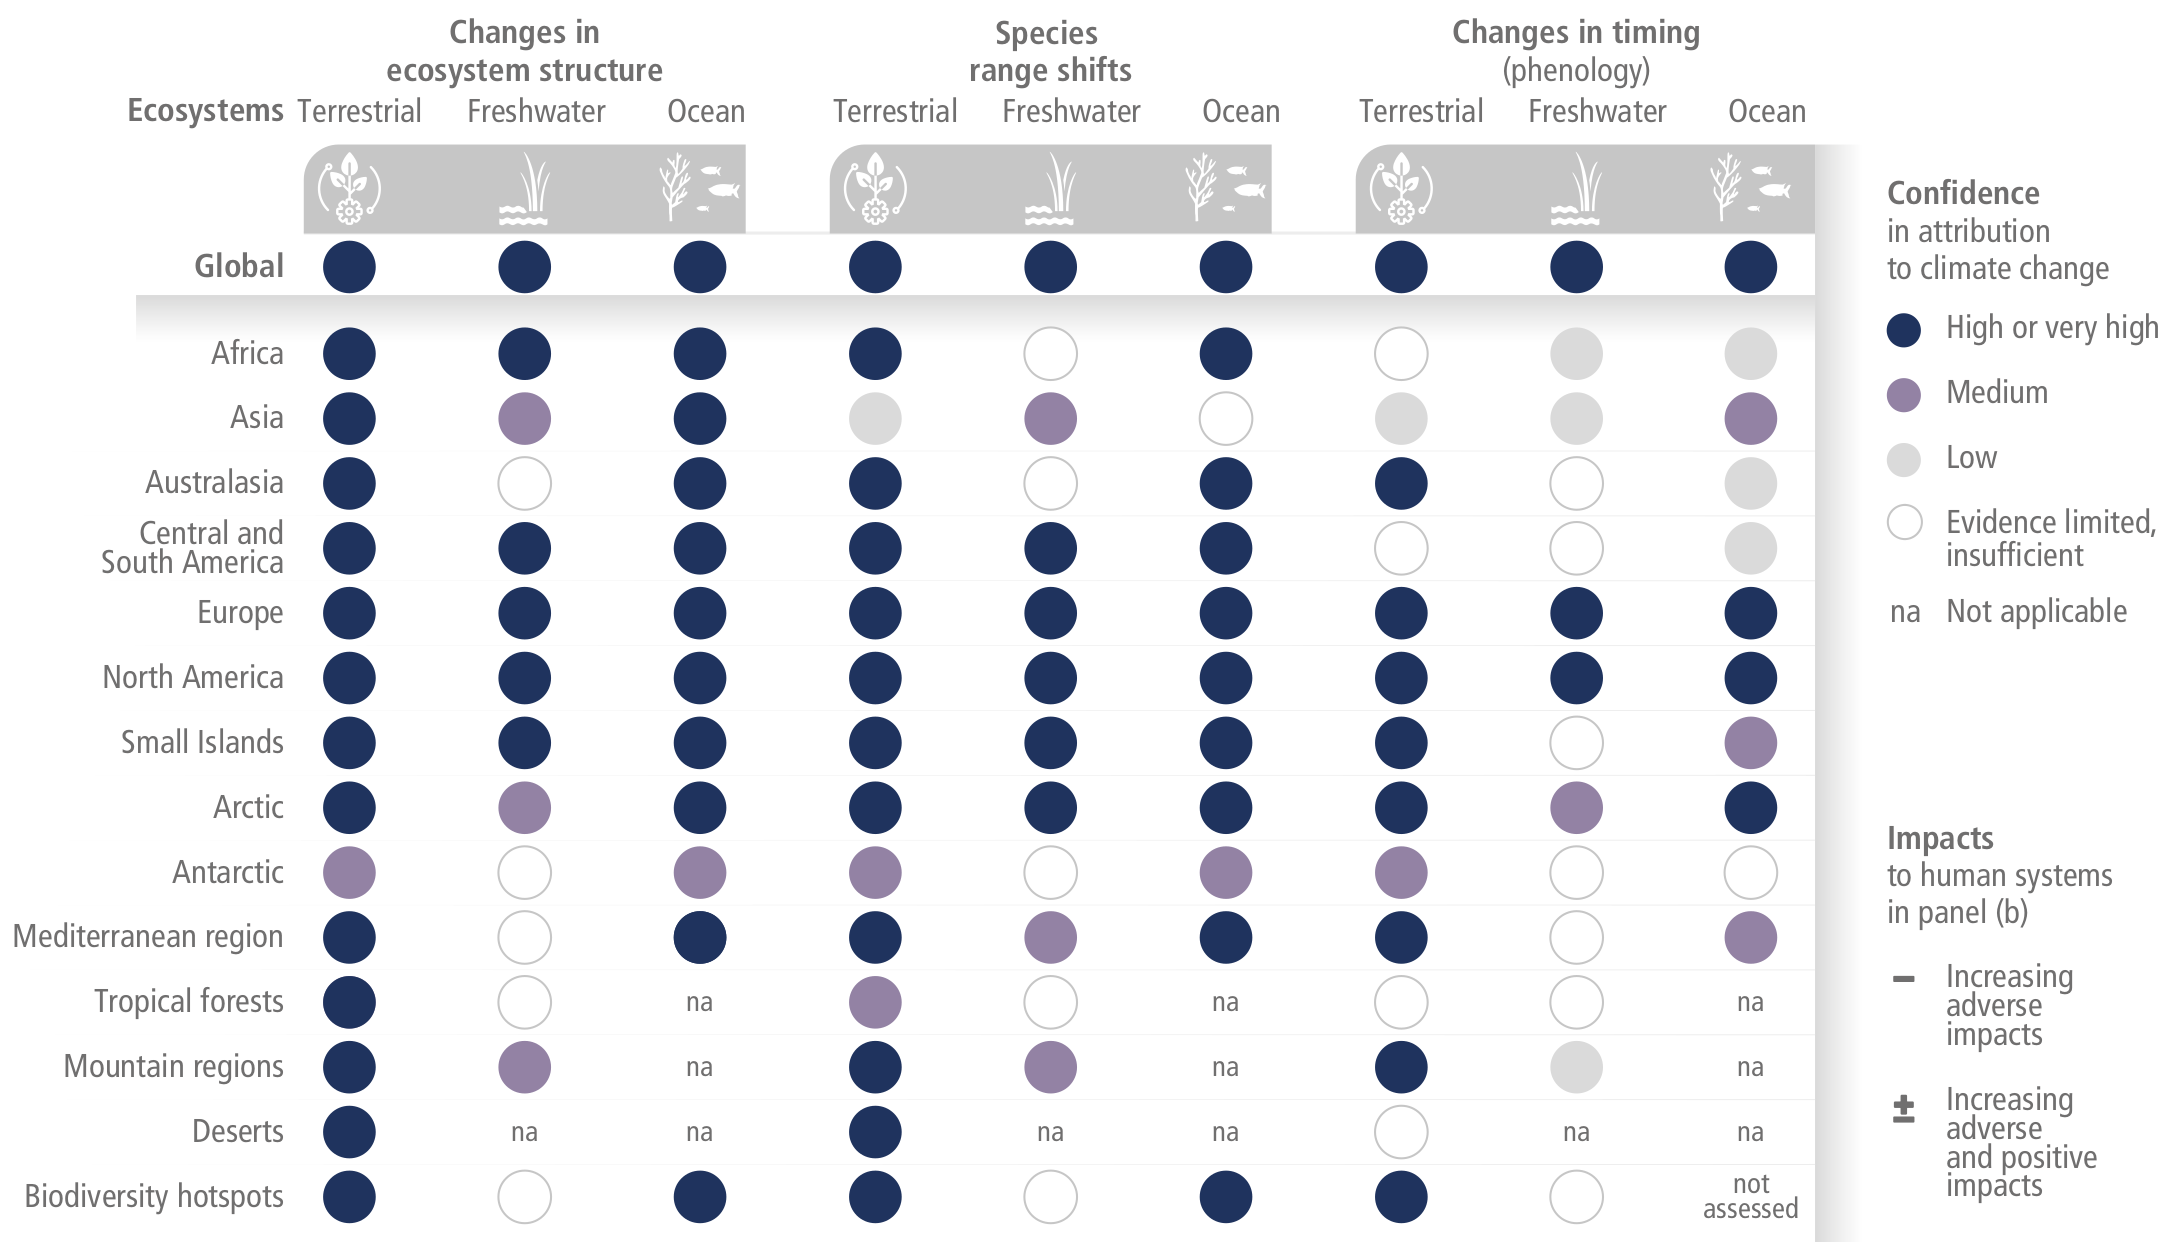
\includegraphics[width=0.8\textwidth]{figs/ipcc-ts3-a.png}
%    \caption{Observed impacts of climate change on ecosystems. From \cite{hans_portner_2022_ts}}
%    \label{fig:ipcc-ts3-a}
%\end{figure}
%
%\begin{figure}[htpb]
%    \centering
%    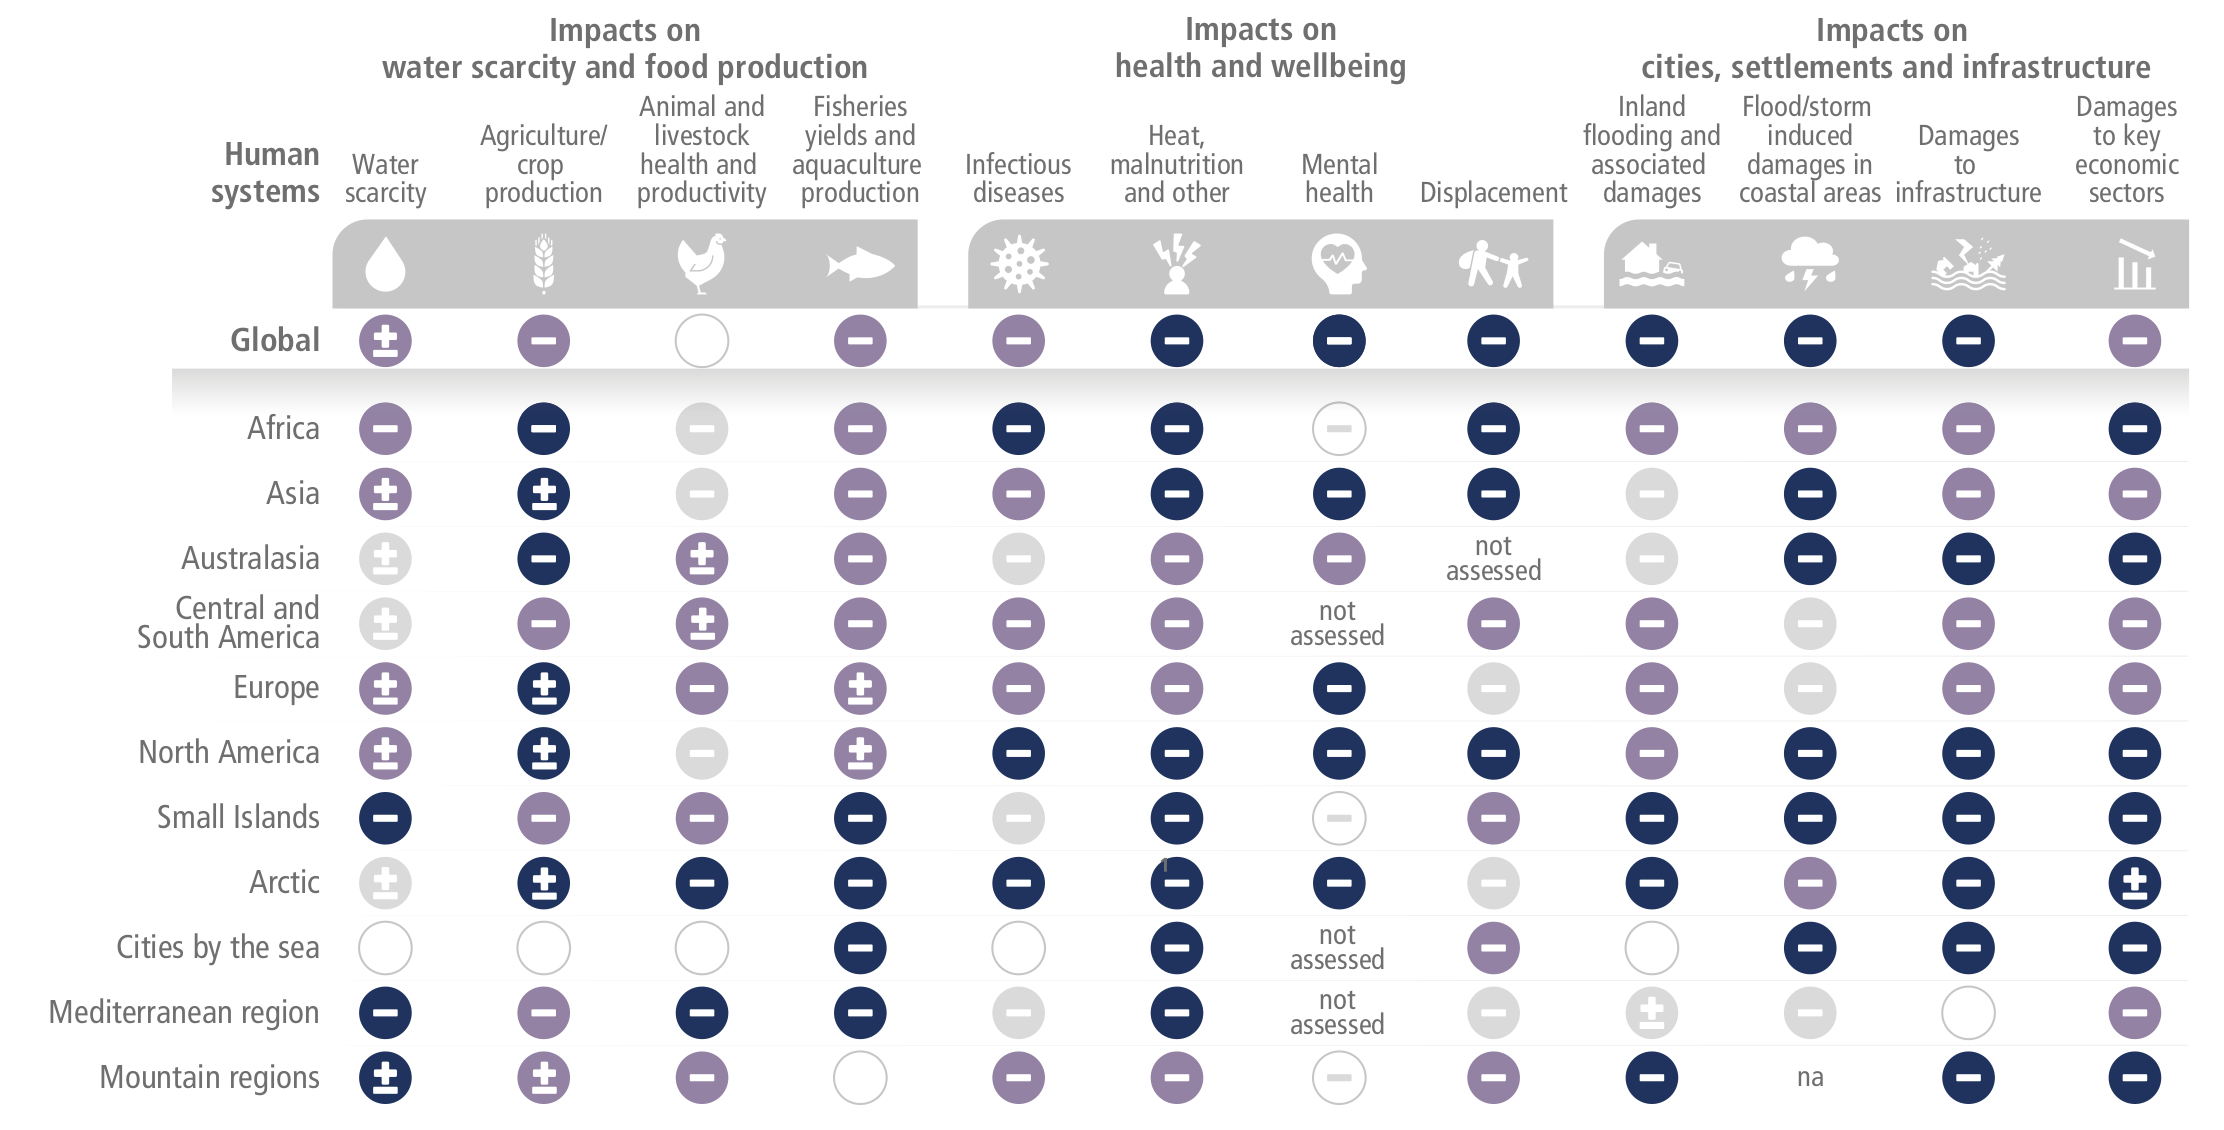
\includegraphics[width=0.8\textwidth]{figs/ipcc-ts3-b.png}
%    \caption{Observed impacts of climate change on human systems. From \cite{hans_portner_2022_ts}}
%    \label{fig:ipcc-ts3-b}
%\end{figure}
%
%Projected impacts of global warming include further ecosystem disruption and
%degradation, risks to global food security, and risks to general well being and
%livelihoods \cite{hans_portner_2022_ts}. Transitioning from fossil
%fuel-based electricity production methods to zero-emission
%\footnote{zero-emissions during operation; there are life-cycle carbon costs
%associated with any form of power production} electricity production methods
%(\textbf{decarbonization}) would contribute significantly to a global \Gls{ghg}
%emission reduction, and, in turn, dampen the effects of global
%warming\cite{minal_pathak_2022_ts}. Our three main options for decarbonization
%are renewables (such as solar, wind, and geothermal), hydropower, and nuclear power. We will
%need all of these technologies working together if we want to successfully
%decarbonize (cite). However, each technology has a specific use case where it works
%best. Solar and wind are best suited for storing up energy for later use on a
%large scale,\footnote{this is a product of the {\it intermittency} of wind and
%solar; solar intensity and wind speed are highly variable and unpredictable
%long term} which can then offset rapid fluctuations in electricity usage.
%Nuclear, hydropower, and geothermal are better suited to provide
%base-load power\cite{eia_electricity_2021}. Geothermal and hydropower are
%limited by geographical features (geothermal activity and elevated water
%sources), making nuclear the most flexible option\footnote{provided a suitable
%coolant exists. The majority of currently operating nuclear power plants are
%water-cooled and thus require a large water source such as a river, lake, or
%ocean.} for a future carbon-free base-load. Therefore, we should
%maintain and develop nuclear power technologies so they can contribute to
%decarbonization efforts.\footnote{despite these positive qualities, nuclear
%power is a divisive technology with legitimate technological and policy
%concerns. Fortunately, many of these concerns have technological and procedural
%solutions}
%
\section{Current and Future Trajectories of Nuclear Power}%
\label{sec:current_and_future_trajectories_of_nuclear_power}
Nuclear power currently constitutes one fifth of US domestic electricity
production and half of US zero-carbon electricity production
\cite{eia_faq_2021} \cite{doene_facts_2021}. The current US nuclear
fleet faces several threats to its future. The most relevant of
these is the state of the electricity market: record-low natural gas prices and
increases in subsidies for renewables without similar compensation for
nuclear make it uncompetitive in the current market and economically unsustainable in the
long term if current conditions continue\footnote{This is a generalization as
the economics of electricity markets is incredibly complex and requires more space that I can give to it
in this thesis to fully appreciate} \cite{szilard_economic_2016}.
%perhaps mention all plants that have been shut down recently?

Assuming that we resolve the economic threats to our current nuclear fleet, they
are -- like all things -- subject to aging and deterioration; at some point in
the future, we will need to shut down and decommission them. 
Nuclear power will be a key player in decarbonization
strategies used in the future. To maintain nuclear power's position in our decarbonization technology
stack, we will need to develop and implement new kinds of nuclear reactors that
are more sustainable, economically competitive, safe, and reliable than their
predecessors. There are several designs that are currently of interest for future
deployment considerations.
%% I want to make this point differently... the conclusion should be that we need new nuclear power tech to ensure we can decarbonize, but I don't feel like the preceding statements smoothly come to that conclusion in the way I have preseneted them here
 
%#\section{Molten Salt Reactors}%
%\label{sec:molten_salt_reactors}
%
%The first generation of nuclear power reactors includes the early prototypes and
%civil deployments in pursuit of cheap and bountiful energy. The second
%generation of reactors was built on top of this momentum, and most reactors
%operating today are from this generation. Following the well publicized and
%documented accidents at Three Mile Island (1976) and Chernobyl (1981) power
%plants, the third generation of nuclear power developed with increased safety
%and reactor lifetime in mind, however these reactors failed to replicate the
%relative success and widespread use of second generation reactors.
This new generation of nuclear power reactors will need to rapidly respond to increasing
electricity consumption and the need for decarbonization. These reactors need
to be built quickly and have widespread use, while maintaining or increasing
fuel efficiency, economic competitiveness, safety, and proliferation resistance.

This is the conclusion that the \Gls{gif} -- a ``co-operative
international endeavor seeking to develop the feasibility and performance of
fourth generation nuclear systems'' \cite{gif_homepage} -- came to in their 2002
roadmap \cite{doe-ne_technology_2002}. The \Gls{gif} selected six reactor
technologies in total. One of them, the \Gls{msr},\footnote{for
this thesis {\it Molten Salt Reactor} refers specifically to the reactor type
where the fissile material is dissolved in in the salt} is of
particular interest due to the unique opportunities and challenges it presents
for new nuclear fuel cycles, proliferation safeguards, and multiphysics
modeling.
%% why the msr??

The \Gls{msr} is so named as it is a nuclear reactor that uses a mixture of
liquid-phase salts as a coolant and solvent for the fuel. Liquid fuel enables
the adoption of {\it online reprocessing} by pumping used fuel out of the
reactor core and pumping fresh or reprocessed fuel back into the reactor core.
\footnote{this concept is known as {\it separations and feeds}} This
enables the removal of undesirable fission products -- neutron absorbers in
particular -- produced by the fission reaction. This also allows for better
utilization of fission neutrons in the fuel. In contrast, while solid-fueled
reactors will shuffle the fuel within the assembly over time, the fission
products remain trapped in the fuel. This can reduce the thermal performance of
the fuel via thermal cracking and absorb neutrons that would otherwise
contribute to the fission reaction. This also means that fuel will be burned
unevenly unless carefully managed

\Gls{msr}s face several technical and logistical challenges before we can
deploy them for civilian power generation. High temperature liquid-phase salt
will steadily corrode metals over time, so the reactor vessel of a \Gls{msr}
must use special corrosion-resistant materials. High temperature salt itself is
extremely hazardous and reacts explosively with moisture, so workers handling
fuel salt must use special procedures and PPE. Remote handling of fuel salt may
be necessary for certain tasks. Even with such challenges, the 
potential benefits of \Gls{msr} technology merit further investigation
into its development.

\Gls{mns} codes will play a critical role in licensing GenIV reactors. In
preparation for \Gls{msr} deployment, both the \Gls{doene} and the \Gls{nrc}
identified several technical gaps in current \Gls{mns} tools that are necessary
for license application reviews
\cite{betzler_modeling_2019} \cite{usnrc_nonlwr_2020-1}. In particular, both the
\Gls{doene} and the \Gls{nrc} have identified fuel composition and its
evolution in \Gls{msr}s to be key modeling features necessary for accident
analysis. 

\section{\Gls{msr} Depletion Codes}%
\label{sec:msr_codes}

To model the changing fuel composition in a \Gls{msr}, there are at least two
processes we must consider:
\begin{enumerate}
    \item Fuel {\it depletion}\footnote{the consumption of fissile material in the fuel and production of fission products via the fission chain reaction} driven my the migration and absorption of neutrons and fuel in the core.
    \item Removal and feed processes of fission products and fuel, respectively.
\end{enumerate}

The Bateman equation describes the process of depletion for any nuclide $i$, or
mathematically, the rate of change of the number density of a nuclide in a nuclear reaction:

\begin{align}
    \label{eq:bateman-1}
    \frac{dN_{i}}{dt} =& \sum_{j} l_{j\to i}\lambda_{j} N_{j} + \gamma_{i} \Sigma^{f}_{j}\phi + \phi N_{i-1} \sigma^{a}_{i-1} - \lambda_{i}N_{i} - N_{i}\sigma^{a}_{i}\phi\\
    \text{where} & \nonumber \\
    N_{x} =& \text{number density for nuclide $x$ $[cm^{-3}]$}\nonumber\\
    l_{j\to i} =& \text{branching ratio for decay mode of nuclide $j$ that produces nuclide $i$ $[-]$}\nonumber\\
    \lambda_{x} =& \text{decay constant of nuclide $x$ $[s^{-1}]$}\nonumber\\
    \gamma_{i} =& \text{fission yield fraction for nuclide $i$ $[-]$}\nonumber \\
    \Sigma^{f}_{j} =& \text{average macroscopic fission cross section for nuclide $j$ $[cm^{-1}]$}\nonumber\\
    \phi =& \text{neutron flux $[cm^{-2}s^{-1}]$}\nonumber\\
    \sigma^{a}_{x} =& \text{neutron absorption cross-section for nuclide $x$ $[cm^{-2}]$}\nonumber\\
\end{align}
    
When solving for $n$ nuclides, we solve the matrix problem
$\frac{d}{dt}N(t) = \mathbf{A}N(t)$, where $N$ is an $n$-vector and
$\mathbf{A}$ contains all the coefficient terms in equation \ref{eq:bateman-1}.
Incorporating removals and feeds into equation \ref{eq:bateman-1} involves the
addition of a time dependent removal factor $r_{i}(t)$ and feed factor
$f_{i}(t)$. The resulting equation describes {\it continuous reprocessing}.
For $n$ nuclides, the matrix problem is then
$\frac{d}{dt}N(t) = \mathbf{A}N(t) + S(t)$, where $S$ is an $n$-vector
containing the sums of the removal and feed terms for each nuclide $i$. The
additional term in the Bateman equation from continuous reprocessing increases
computational cost and implementation difficulty and may require a different
set of preconditioners for numerical stability and convergence.

Alternatively, one could run a depletion simulation, perform the removals and
feeds in an external application on the resulting material composition, and run
another depletion simulation on the reprocessed composition. This procedure
models {\it batch-wise reprocessing}, in which material from the core is
reprocessed at regular intervals rather than continuously. Batch-wise
reprocessing enables flexibility in the choice of depletion solver, as an
external software tool can perform the reprocessing step and feed the results
back into the depletion solver.\footnote{this kind of coupling comes with its
own challenges, which are beyond the scope of this thesis}

\SaltProc\cite{rykhlevskii_saltproc_2018}, the focus of this thesis, uses a
batch-wise reprocessing approach to model the fuel composition in an \Gls{msr}
and uses \SerpentTWO\cite{leppanen_serpent_2014} to run depletion simulations.
\SaltProc is unique among its peers as an open source project\footnote{There are
other software projects that model fuel composition in \Gls{msr}s. Notably,
\ChemTriton\cite{betzler_molten_2017} -- a python script for \SCALE/\TRITON --
is functionally similar to \SaltProc. Section 1.2 in
\cite{rykhlevskii_fuel_2020} and section 4.2 in \cite{rykhlevskii_advanced_2018}
provide a high-level summary of other recent efforts}.

Historically, software used in licensing, \gls{rnd}, and \gls{ent} efforts in
the nuclear field have been closed source and proprietary. For \Gls{rnd} and
\Gls{ent} efforts in particular, the licensing process can bring collaborative
efforts to a grinding halt. Using \gls{cc}s in scientific publications and
research presents barriers to reproducibility and the ability of external
verification of results.
    
Regulatory bodies will require new software features (and, in some cases,
entirely new software tools) to effectively and efficiently perform licensing
activities for the next generation of advanced reactor designs
\cite{usnrc_nonlwr_2020-1}. Many of the open source tools emerging in the
past decade (e.g., \OpenMC\cite{romano_openmc_2015}) have the advantage over
their legacy \Gls{cc} ancestors (e.g., \SerpentTWO \cite{leppanen_serpent_2014})
of using best-practices for software development. Thus, the features
and tools required may be more readily implementable and usable in open source
projects than in closed codes.
    
We are entering the era of \gls{oss} purpose-built for nuclear
science and engineering applications. The number of open source projects in this
field
(\ONIX\cite{de_troullioud_de_lanversin_onix_2021}, \OpenMC,
\NJOYTWOONE\cite{noauthor_njoy21_2022}, \Cyclus\cite{noauthor_cyclus_2022}, to
name a few\footnote{the awesome-nuclear repository on GitHub
\cite{romano_awesome_2022} has good list of nuclear-related open source software
projects.}) is growing in recognition of the need for distributable,
high-quality, and transparent software tools. The
\Gls{iaea} facilitated \Gls{oncore} initiative \cite{fiorina_initiative_2021} is the best
example of the push towards \Gls{oss}, as seen in the mission
statement: to
``[promote] development and application of open-source multi-physics simulation
tools to support research, education, and training for analysis of advanced
nuclear power reactors'' \cite{iaea_open-source_2022}. 


\section{Objectives}%
\label{sec:objectives}

While \SaltProc itself is open source, \SerpentTWO is not. \OpenMC recently
added a \verb.deplete. module for fuel depletion simulations, meaning it is now
possible to have a fully open-source stack of dependencies for \SaltProc.
In this spirit, I have added support for \OpenMC to \SaltProc. \OpenMC support improves
the accessibility and usability of \SaltProc, and I hope that researchers
interested in \Gls{msr}s begin using and contributing to the tool.

This Master's thesis has two primary objectives
\begin{enumerate}
    \item Refactor \SaltProc to enable \OpenMC support, as well as enable
        easier implementation for other monte-carlo depletion codes in the
        future. 
    \item Verify the implementation on a \Gls{csg} model of the \Gls{msbr}\footnote{See
        Chapters 2 and 4 for a discussion of this choice.}
\end{enumerate}

It is my hope that with the addition of \OpenMC support, \SaltProc can have a
lower barrier-of-entry for researchers and students. 

The structure of this thesis is as follows:
\begin{itemize}
    \item Chapter \ref{ch:chapter2} describes the structure of \SaltProc and process of
        implementing support for \OpenMC in the context of past and current
        \Gls{msr} modeling efforts.
    \item Chapter \ref{ch:chapter3} describes the updated code structure and restates the
        formal mathematical representation of the reprocessing used in the
        SaltProc.
    \item Chapter \ref{ch:chapter4} describes the reactor design for verification purposes and
        specifies the inputs and settings.
    \item Chapter \ref{ch:chapter5} presents the results of the verification study and
        discusses their implications.
    \item Chapter \ref{ch:chapter6} summarizes the results, their implications, and suggests
        avenues for future work.
\end{itemize}


\chapter{Molten Salt Reactor Modeling}%
\label{cha:msr_modeling}
%% lit review goes here
Much of our knowledge about \Gls{MSR}s come from experiements on a test reactor called the \Gls{MSRE} conducted at \Gls{ORNL} in the 1960s, which demonstrated the viability of the \Gls{MSR} concept for use in civillian power programs \cite{haubenreich_experience_1970} \cite{rosenthal_molten-salt_1970}.
%% Give brief description of the MSRE
%% cite a bunch of MSRE ORNL work.

The \Gls{MSRE} reactor to this day remains one of the few \Gls{MSR}s to operate.
%% Maybe briefly mention other historical MSRs?

As of writing this thesis, there are no \Gls{MSR}s currently in operation. Therefore, we must entirely rely on computational and/or surrogate models to further study \Gls{MSR} physics. The \Gls{MSRE} is a popular choice for computational models due to the availability of experimental data to compare results against. For example, Roelofs et al used the system thermal hydraulics code SPECTRA to model steady state parameters of the fuel-salt, \Gls{DNP} drift, and various fission product behaviors
in comparison with actual MSRE data \cite{roelofs_molten_2021}.  Podila et al performed a \Gls{CFD} simulation of the \Gls{MSBR} core to investigate the ability of \Gls{CFD} to predict 3D effects in this kind of reactor\cite{podila_cfd_2019}. 
%cite some MSRE studies
In addtion to the \Gls{MSREBR}, the \Gls{MSFR}(cite) and \Gls{MSBR}(cite), while conceptual, are well developed and have many associated studies. See Table () for a summary. These efforts illustrate that \Gls{MSR} modeling encompasses a wide range of physics domains.

Park et al perfomred a whole core analysis of the \Gls{MSBR} using MCNP6 with additional depletion and reprocessing using CINDER90 and a custom Python script \cite{park_whole_2015}.

\section{Modeling depletion in \Gls{MSR}s}
Recall in Sections
\ref{sec:molten_salt_reactors} and \ref{sec:msr_codes} we introduced the concepts of fuel depletion and removal and feed processes, and established the importance of modeling fuel depletion to \Gls{MSR} lisencing. Degletion codes in the past have shown good behavior when compared with experiment, although most of these models are . In M Table (table) summarizes some available software tools that can model depletion in \Gls{MSR}s.

%% Discuss briefly results from depletion papers

The to accurate \Gls{MSR} models.
A survey of some recent \Gls{MSR}s modeling efforts are summarized in Table (table?). 

%% talk about internal tools that natively support dpeletion (serpent, openmc, mention shift)

%% then talk about external tools (SaltProc, ChemTrition)

We are focused on OpenMC and Serpent because\ldots
%% talk about saltproc in it's current state, the gaps that exist
%% lead into discussion about why it's important to add openmc 
%% capabilities to SaltProc. Also mention the differnces in 
%% Serpent2 and OpenMC cross section handling and how this
%% adds capability to the SaltProc tool


%% Move this to the next chapter
\section{Sotware Overview and Development}
\label{sec:soft_dev}
A major component of this work was restructuring of the SaltProc code and implementation of OpenMC. In this section, I will provide a high level overview of my development process and go into detail where necessary. The release notes contain more details for those interested.
\subsection{SaltProc}%
\label{sub:saltproc}

SaltProc\cite{rykhlevskii_saltproc_2018} is an open source Python package that simulates on-line reprocessing via a batch-wise approach\footnote{Material is moved to or from the core at specific time intervals} in liquid-fueled \Gls{msr}s. More precisely, SaltProc manages material flows and separation processes on nuclides in the fuel. SaltProc relies on external codes to simulate fuel depletion.

The first version of SaltProc (v0.1) was a simple Python 2.7 package that used SERPENT 2 for the fuel depletion simulations. A single Python file contained all functions; separation processes applie dto  used an implicit 100\% efficiency \cite{rykhlevskii_advanced_2018}. The structure of SaltProc v0.1 did not lend itsef easily to development of more sophisticated treatments of reprocessing. This led to the release of Saltproc v0.2, in which the entire codebase was refactored into an object oriented
context in Python 3. The addition of new functionality in the \verb.Process. classes enabled more sophisticated treatment of online reprocessing \cite{rykhlevskii_fuel_2020} 

SaltProc v0.3 saw the implementation of processes for gas sparging and separation to more accurately simulate the MSBR, as well as additional refactoring to better follow OOP concepts.

\subsubsection{Preparing for OpenMC support}%
While v0.2 and v0.3 saw most of SaltProc refactored for OOP, before I could implement OpenMC support, I needed to resolve the following issues:
\begin{enumerate}
    \item Relocate several functions to have better separation of concerns
    \item Overhaul the SaltProc input file format giving users more control over their simulations
    \item Generalize docstrings\footnote{Since SaltProc was initally written as a script wrapped around Serpent2, many of the docstrings explicitly referenced Serpent2.}
    \item Improve function and variable names
\end{enumerate}
I implemented these changes as part of the 0.4.0 release. The changes in that release changed the API, making 0.4.0 incompatible with previous verions of SaltProc.
% consider talking about automation?

\section{OpenMC}%
\label{sub:openmc}

OpenMC \cite{romano_openmc_2015} is an open source Monte Carlo particle transport code. The \Gls{crpg} at \Gls{mit} started developing OpenMC back in 2011 with a focus on scalability for exascale computing. Since that time, developers new and old contributed features (cite?) and fixes to the tool expanding its scope and use cases. Notable features of OpenMC (as of version 0.12.1) are as follows \cite{homepage_openmc_2022}:
\begin{itemize}
    \item Support for fixed source, $k$-eigenvalue, and subcritical neutron multiplication cacluclations.
    \item Support for \Gls{csg} and \Gls{cad} geometry.
    \item Support for both continuous and multigroup transport calculations.
    \item Support for parallel execution via MPI and OpenMP.
    \item Geometry visualization through the Python API.
\end{itemize}
The tool is now quite mature and feature-rich, and is a legitmate alternative to it's closed-source counterparts in many cases.

Recently, depletion and photon transport were added by (who?)... The new depletion feature enables us to couple OpenMC to SaltProc and a fully open-source stack.

\subsection{Adding OpenMC to SaltProc}%
\label{sub:adding_openmc_to_saltproc}

\chapter{Software Description}
Development on \SaltProc to enable use with \OpenMC consitutes a major portion
of this thesis. In this chapter, I will provide a high level overview
of my development process.\footnote{The release notes
contain more details for those interested} I will also provide an updated
description of the code structure using the new API. 

\section{SaltProc development history}%
\label{sub:saltproc-hisory}

\SaltProc\cite{rykhlevskii_saltproc_2018} is an open source Python package that
simulates on-line reprocessing via a batch-wise approach\footnote{Material is
moved to or from the core at specific time intervals} in liquid-fueled
\Gls{msr}s. More precisely, \SaltProc manages material flows and separation
processes on nuclides in the fuel. \SaltProc relies on external codes to simulate
fuel depletion.

The first version of \SaltProc (v0.1) was a simple Python 2.7 package that used
\SerpentTWO for the fuel depletion simulations. A single Python file contained
all functions; separation processes applie dto  used an implicit 100\%
efficiency \cite{rykhlevskii_advanced_2018}. The structure of \SaltProc v0.1 did
not lend itsef easily to development of more sophisticated treatments of
reprocessing. This led to the release of \SaltProc v0.2, in which the entire
codebase was refactored into an object oriented context in Python 3. The
addition of new functionality in the \verb.Process. classes enabled more
sophisticated treatment of online reprocessing \cite{rykhlevskii_fuel_2020} 

\SaltProc v0.3 saw the implementation of processes for gas sparging and
separation to more accurately simulate the \gls{msbr}, as well as additional
refactoring to better follow OOP concepts.

While v0.2 and v0.3 saw most of \SaltProc refactored for OOP, before I could
implement \OpenMC support, I needed to resolve the following issues:
\begin{enumerate}
    \item Relocate several functions to have better separation of concerns
    \item Overhaul the \SaltProc input file format giving users more control over their simulations
    \item Generalize docstrings\footnote{Since \SaltProc was initally written as a script wrapped around Serpent2, many of the docstrings explicitly referenced Serpent2.}
    \item Improve function and variable names
\end{enumerate}
I implemented these changes as part of the 0.4.0 release. The changes in that
release changed the API, making 0.4.0 incompatible with previous verions of \SaltProc.

\SaltProc v0.5.0 added full support for \OpenMC, overhauled the test suite, and included additional API changes.

% consider talking about automation?

\section{OpenMC}%
\label{sub:openmc}

OpenMC \cite{romano_jpenmc_2015} is an open source Monte Carlo particle
transport code. The \Gls{crpg} at \Gls{mit} started developing OpenMC back in
2011 with a focus on scalability for exascale computing. Since that time,
developers new and old contributed features (cite?) and fixes to the tool
expanding its scope and use cases. Notable features of OpenMC (as of version
0.13.1) are as follows \cite{homepage_openmc_2022}:
\begin{itemize}
    \item Support for fixed source, $k$-eigenvalue, and subcritical neutron multiplication cacluclations.
    \item Support for \Gls{csg} and \Gls{cad} geometry.
    \item Support for both continuous and multigroup transport calculations.
    \item Support for parallel execution via MPI and OpenMP.
    \item Geometry visualization through the Python API.
    \item Transport-coupled and transport-independent depletion
\end{itemize}

\section{SaltProc v0.5.0}
\label{sec:saltproc-detail}

\subsection{Feeds and Separations}
\SaltProc models separations and feeds using three different data structures:


\paragraph{Material flows}
    A material flow represents a material with a given
    volume, density, and temperature, and nuclide composition.
    It can also include information such as void fraction. \verb.Materialflow.
    objects contain the prior mentioned quantities as attributes, as well as
    methods to perform the following:
    \begin{itemize}
        \item Add two \verb.Materialflow. objects together
        \item Multiply a \verb.Materialflow. object by a constant
    \end{itemize}
    \verb.Materialflow. objects are used to store information about materials
    in reprocessing as well as materials being fed into the system.

\paragraph{Processes}
    A process is an abstraction of chemical separation, extraction, or some
    other removal. Two processes commonly used in \Gls{msr}s include
    extracting metals using gas sparging and filtering. In \SaltProc,
    \verb.Process. objects contain data and functions to perform their
    associated processing task. At a minimum, a \verb.Process. object includes
    the following
    \begin{itemize}
        \item A mass flowrate, $\dot{m}$, that specifies the mass of fuel salt a process can operate on per unit time
        \item An extraction efficiency, $\epsilon$, for target element(s). This can be a constant value or a function.
        \item A method to apply the process on a \verb.Materialflow. object. 
    \end{itemize}

\paragraph{Graphs}
    A graph is a mathematical object that connects {\it nodes}\footnote{the
    terms verices and points are also used} with {\it edges}. More formally,
    a graph is a pair of sets, $(V, E)$, where
    \begin{itemize}
        \item $V$ is a set whose elements are called nodes
        \item $E$ is a set whose elements are pairs of elements in $V$
    \end{itemize}
    A directed graph is a graph where the elements are ordered pairs of elements
    in $V$. This gives the edges a direction. \SaltProc uses directed graphs to
    model the order and path in which processes operate on materials.
        
Processes and feesd are defined in one JSON input file, and the graph linking
processes is  defind in a DOT file. The process graph must be directed and
acyclic in order to work with \SaltProc v0.5.0. At runtime, \SaltProc reads this
input file to create \verb.Process. objects for each item in the file. Every
process file must have at lest a \verb.core_outlet. and \verb.core_inlet.
Process.

\subsection{Material reprocessing}
Recall that \SaltProc uses a {\it batchwise} reprocessing scheme.

Let $\mathbf{n}(t)^{j}$ denote the nuclide mass vector for depletable material
$j$ as function of time. For each depletable material $j$, the depletion solver numerically
integrates the equation

\begin{equation}
    \frac{d\mathbf{n}^{j}(t)}{dt} = \mathbf{A}(\mathbf{n}^{j}(t), t)
\end{equation}

from time $i$ to time $i+1$ to get $\mathbf{n}^{j}(i+1)$, where $A$ is the
depletion matrix. The specific details of integration are alredy covered in
numerous other works (cite some here). This is sequence is called a {\bf depletion
step}.

Now, let the mass and volume of depletable material $j$ be
$m^{j}$ and $V^{j}$ respectively. Let the mass flowrate of process $p$ be
$\dot{m}_{p}$. At the end of each depletion step, \SaltProc constructs process
paths from the process graph defined in the DOT file, and sequentially applies
each proceess $p$ in each path $r$ to the relevant materials to obtain thru
and waste streams for each material. \SaltProc tracks the mass and nuclide vector for both thru and waste streams. For thru
streams, \SaltProc also tracks the volume and mass flowrate. For every node
$p\in[0,l]$ where $0$ represents the core outlet and $l$ represents the core
inlet, in the path $r$, for the thru streams we have

% still need burnup, temp, density, void frac
\begin{equation}
    \mathbf{n}^{j}_{\text{thru, }p,r} = \mathbf{n}^{j}_{\text{thru, }p-1,r} (1 - \mathbf{\epsilon}^{j}_{p,r})
\end{equation}
\begin{equation}
    m^{j}_{\text{thru, } p,r} = \alpha_{p} m^{j}_{\text{thru, }p-1,r} - m^{j}_{\text{waste, }p,r}
\end{equation}
\begin{equation}
    V^{j}_{\text{thru, }p,r} = \alpha_{p}V^{j}_{\text{thru, }p-1,r}
\end{equation}
where 
\begin{equation}
    \alpha_{p,r} = \frac{\dot{m}_{p,r}}{\dot{m}_{\text{outlet}}}
\end{equation}
and the inital conditions are 
\begin{equation}
    \mathbf{n}^{j}_{\text{thru, }0,r} = \mathbf{n}^{j}(i+1)
\end{equation}
\begin{equation}
    m^{j}_{\text{thru, }0,r} = \rho^{j}(i+1)V^{j}(i+1)
\end{equation}
\begin{equation}
    V^{j}_{\text{thru, }0,r} = V^{j}(i+1)
\end{equation}
Similarly, for the waste streams, we have
\begin{equation}
    \mathbf{n}^{j}_{\text{waste, }p,r} = \mathbf{n}^{j}_{\text{thru, }p-1,r} \cdot \mathbf{\epsilon}^{j}_{p,r}
\end{equation}
\begin{equation}
    m^{j}_{\text{waste, }p,r} = \alpha_{p,r} m^{j}_{\text{thru, }p-1,r} \langle\mathbf{1},\mathbf{n}^{j}_{\text{waste, }p,r}\rangle
\end{equation}
SaltProc does not currently track the volume and mass flowrate of waste streams.
In practice, since it is very difficult to separate individual isotopes,
SaltProc only allows extraction efficiencies to be defined for elements. So for
any isotope $a$ of xenon,
$\epsilon_{\ce{^{a}Xe}} = \epsilon_{\ce{^{a^{\prime}}Xe}}$  where
$a^{\prime} \in \text{isotopes of Xe}$

After the recursive computation, \SaltProc sums thru and waste streams over all
paths to get the total thru stream at the inlet, and the total waste stream at
the inlet which represents all material removed during reprocessing.
\begin{equation}
    \mathbf{n}^{j}_{\text{thru, inlet, net}} = \frac{\sum_{r} m^{j}_{\text{thru, inlet, }r} \mathbf{n}^{j}_{\text{thru, inlet, }r}}{\sum_{r} m^{j}_{\text{thru, inlet, }r}}
\end{equation}
\begin{equation}
    \mathbf{n}^{j}_{\text{waste, inlet, net}} = \frac{\sum_{r} m^{j}_{\text{waste, inlet, }r} \mathbf{n}^{j}_{\text{waste, inlet, }r}}{m^{j}_{\text{waste, inlet, }r}}
\end{equation}

Before running the next depletion step, for any material that has an associated
feed material defined, \SaltProc will add an amount of the feed material
equivalent to the removed mass so that the mass of fuel salt undergoing depletion
remains constant.
For feed $j'$ corresponding to material $j$, we have
\begin{equation}
    \mathbf{n}^{j}_\text{filled} = \frac{m^{j}_{\text{thru, }l}\mathbf{n}^{j}_{\text{thru, inlet, net}} +  m^{j}_{\text{removed}}\mathbf{n}^{j'}}{m^{j}_{\text{thru,}0}}
\end{equation}

where 
\begin{equation}
    m^{j}_{\text{removed}} = m^{j}_{\text{thru,}0} - m^{j}_{\text{thru, } l}
\end{equation}

\chapter{Model Description}
\label{ch:chapter4}
As mentioned in Section \ref{sec:objectives}, I am using a \Gls{csg} model of
the \Gls{msbr} \cite{robertson_conceptual_1971} to verify my \OpenMC
implementation in \SaltProc.

The \Gls{msbr} design is the result of a design study of a single-fluid
\Gls{msr} following the success of the \Gls{msre}
\cite{haubenreich_experience_1970} \cite{rosenthal_history_1970}.

I picked the \Gls{msbr} for two reasons:
\begin{enumerate}
    \item Several papers studying the \Gls{msbr} exist,\footnote{see Chapter
    \ref{ch:chapter2} for a discussion of these papers} enabling qualitative
    results comparison.
    \item Rykhlevskii created a \SerpentTWO \Gls{csg} model and the processing
    system graph for the \Gls{msbr} based on the specifications in
    \cite{robertson_conceptual_1971} for use in \SaltProc
    v0.3.0 \cite{rykhlevskii_fuel_2020}. The models used in this work are derived
    from Rykhlevskii's model.
\end{enumerate}

Most of the discussion below summarizes and condenses the information in
Robertson et al. (1971) and compares it to the \Gls{csg} model. Unless otherwise
specified, there are no differences between the model used in this work and in
\cite{rykhlevskii_fuel_2020}\footnote{The relevant component of Reference
\cite{rykhlevskii_fuel_2020}, Chapters 2 and 3, are based on Reference
\cite{rykhlevskii_modeling_2019}. I may use these references interchangeably}. I
will only describe the following reactor systems that are relevant to my
validation study\footnote{A complete description of the entire \Gls{msbr} system
can be found in Robertson et al. (1971) \cite{robertson_conceptual_1971}.
Interested readers should focus on Table S.1, Sections 3.4, 3.1, and 3.5 in
Robertson et al. (1971) for further details and design considerations.}: the
fuel salt, the reactor core, and the salt reprocessing system.

\begin{figure}[htpb] 
    \centering
    \subfloat[][]{
        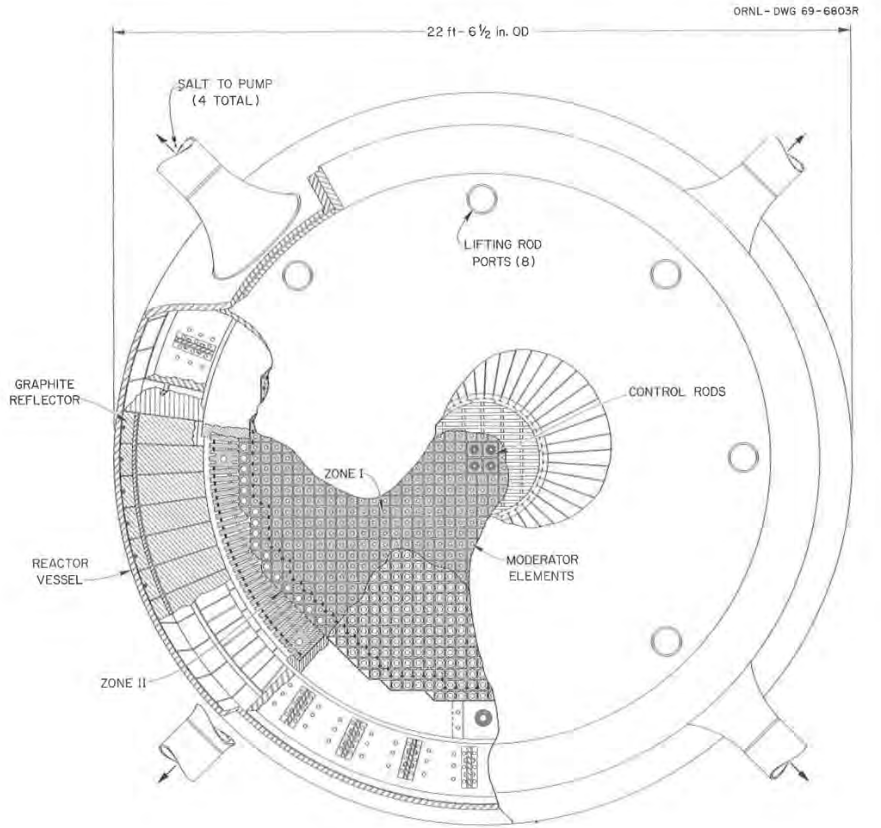
\includegraphics[width=0.5\linewidth]{figs/ch4/msbr_full_xy_ref.png}
        \label{fig:msbr-ref-xy}
    }
    \subfloat[][]{
        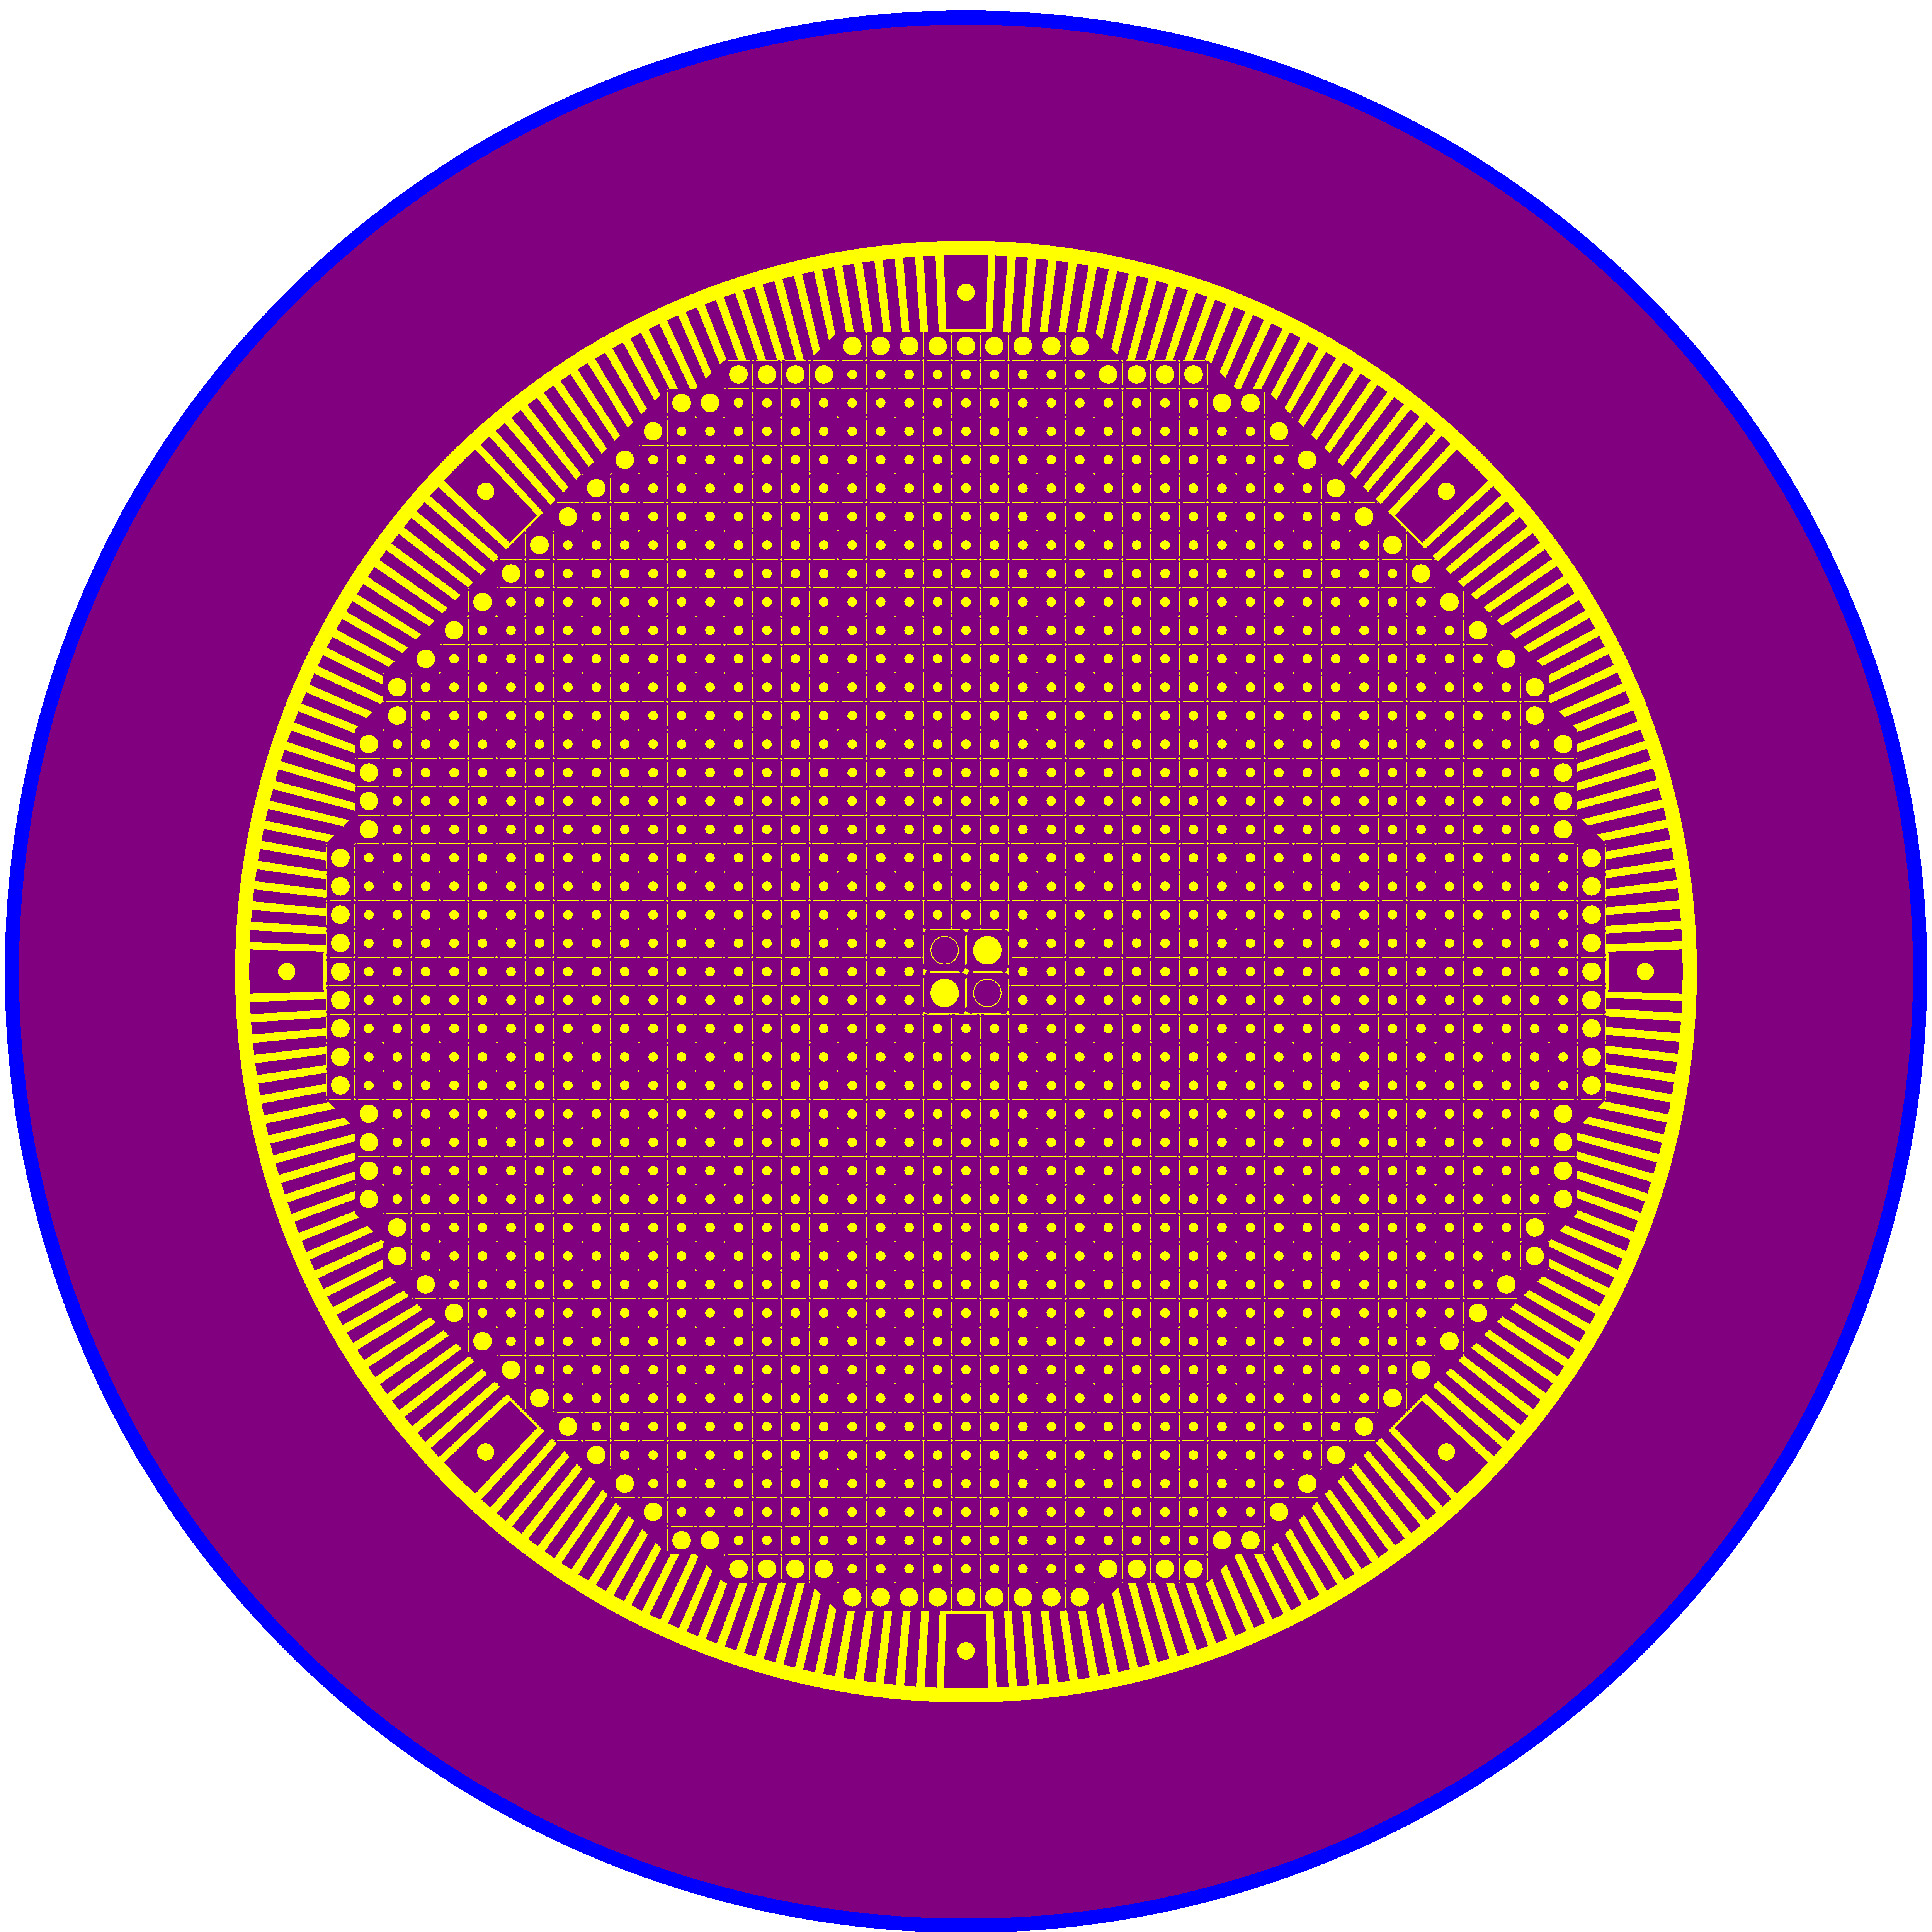
\includegraphics[width=0.5\linewidth]{figs/ch4/msbr_full_xy_openmc.png}
        \label{fig:msbr-model-xy}
    }
    \\
    \subfloat[][]{
        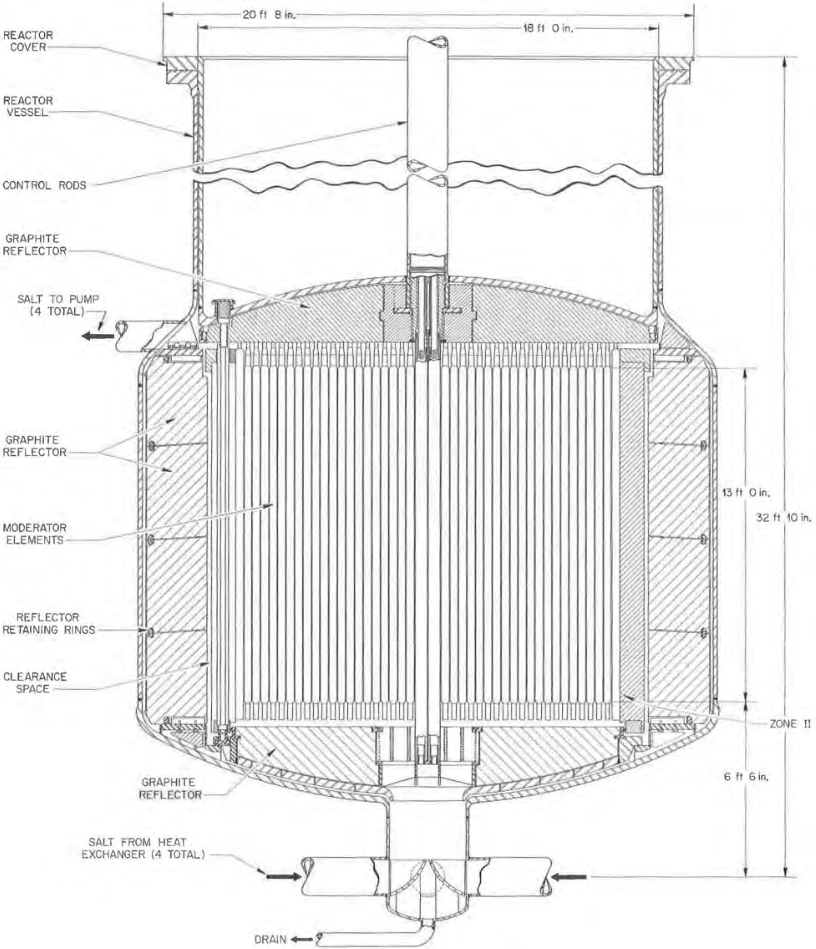
\includegraphics[width=0.5\linewidth]{figs/ch4/msbr_full_xz_ref.png}
        \label{fig:msbr-ref-xz}
    }
    \subfloat[][]{
        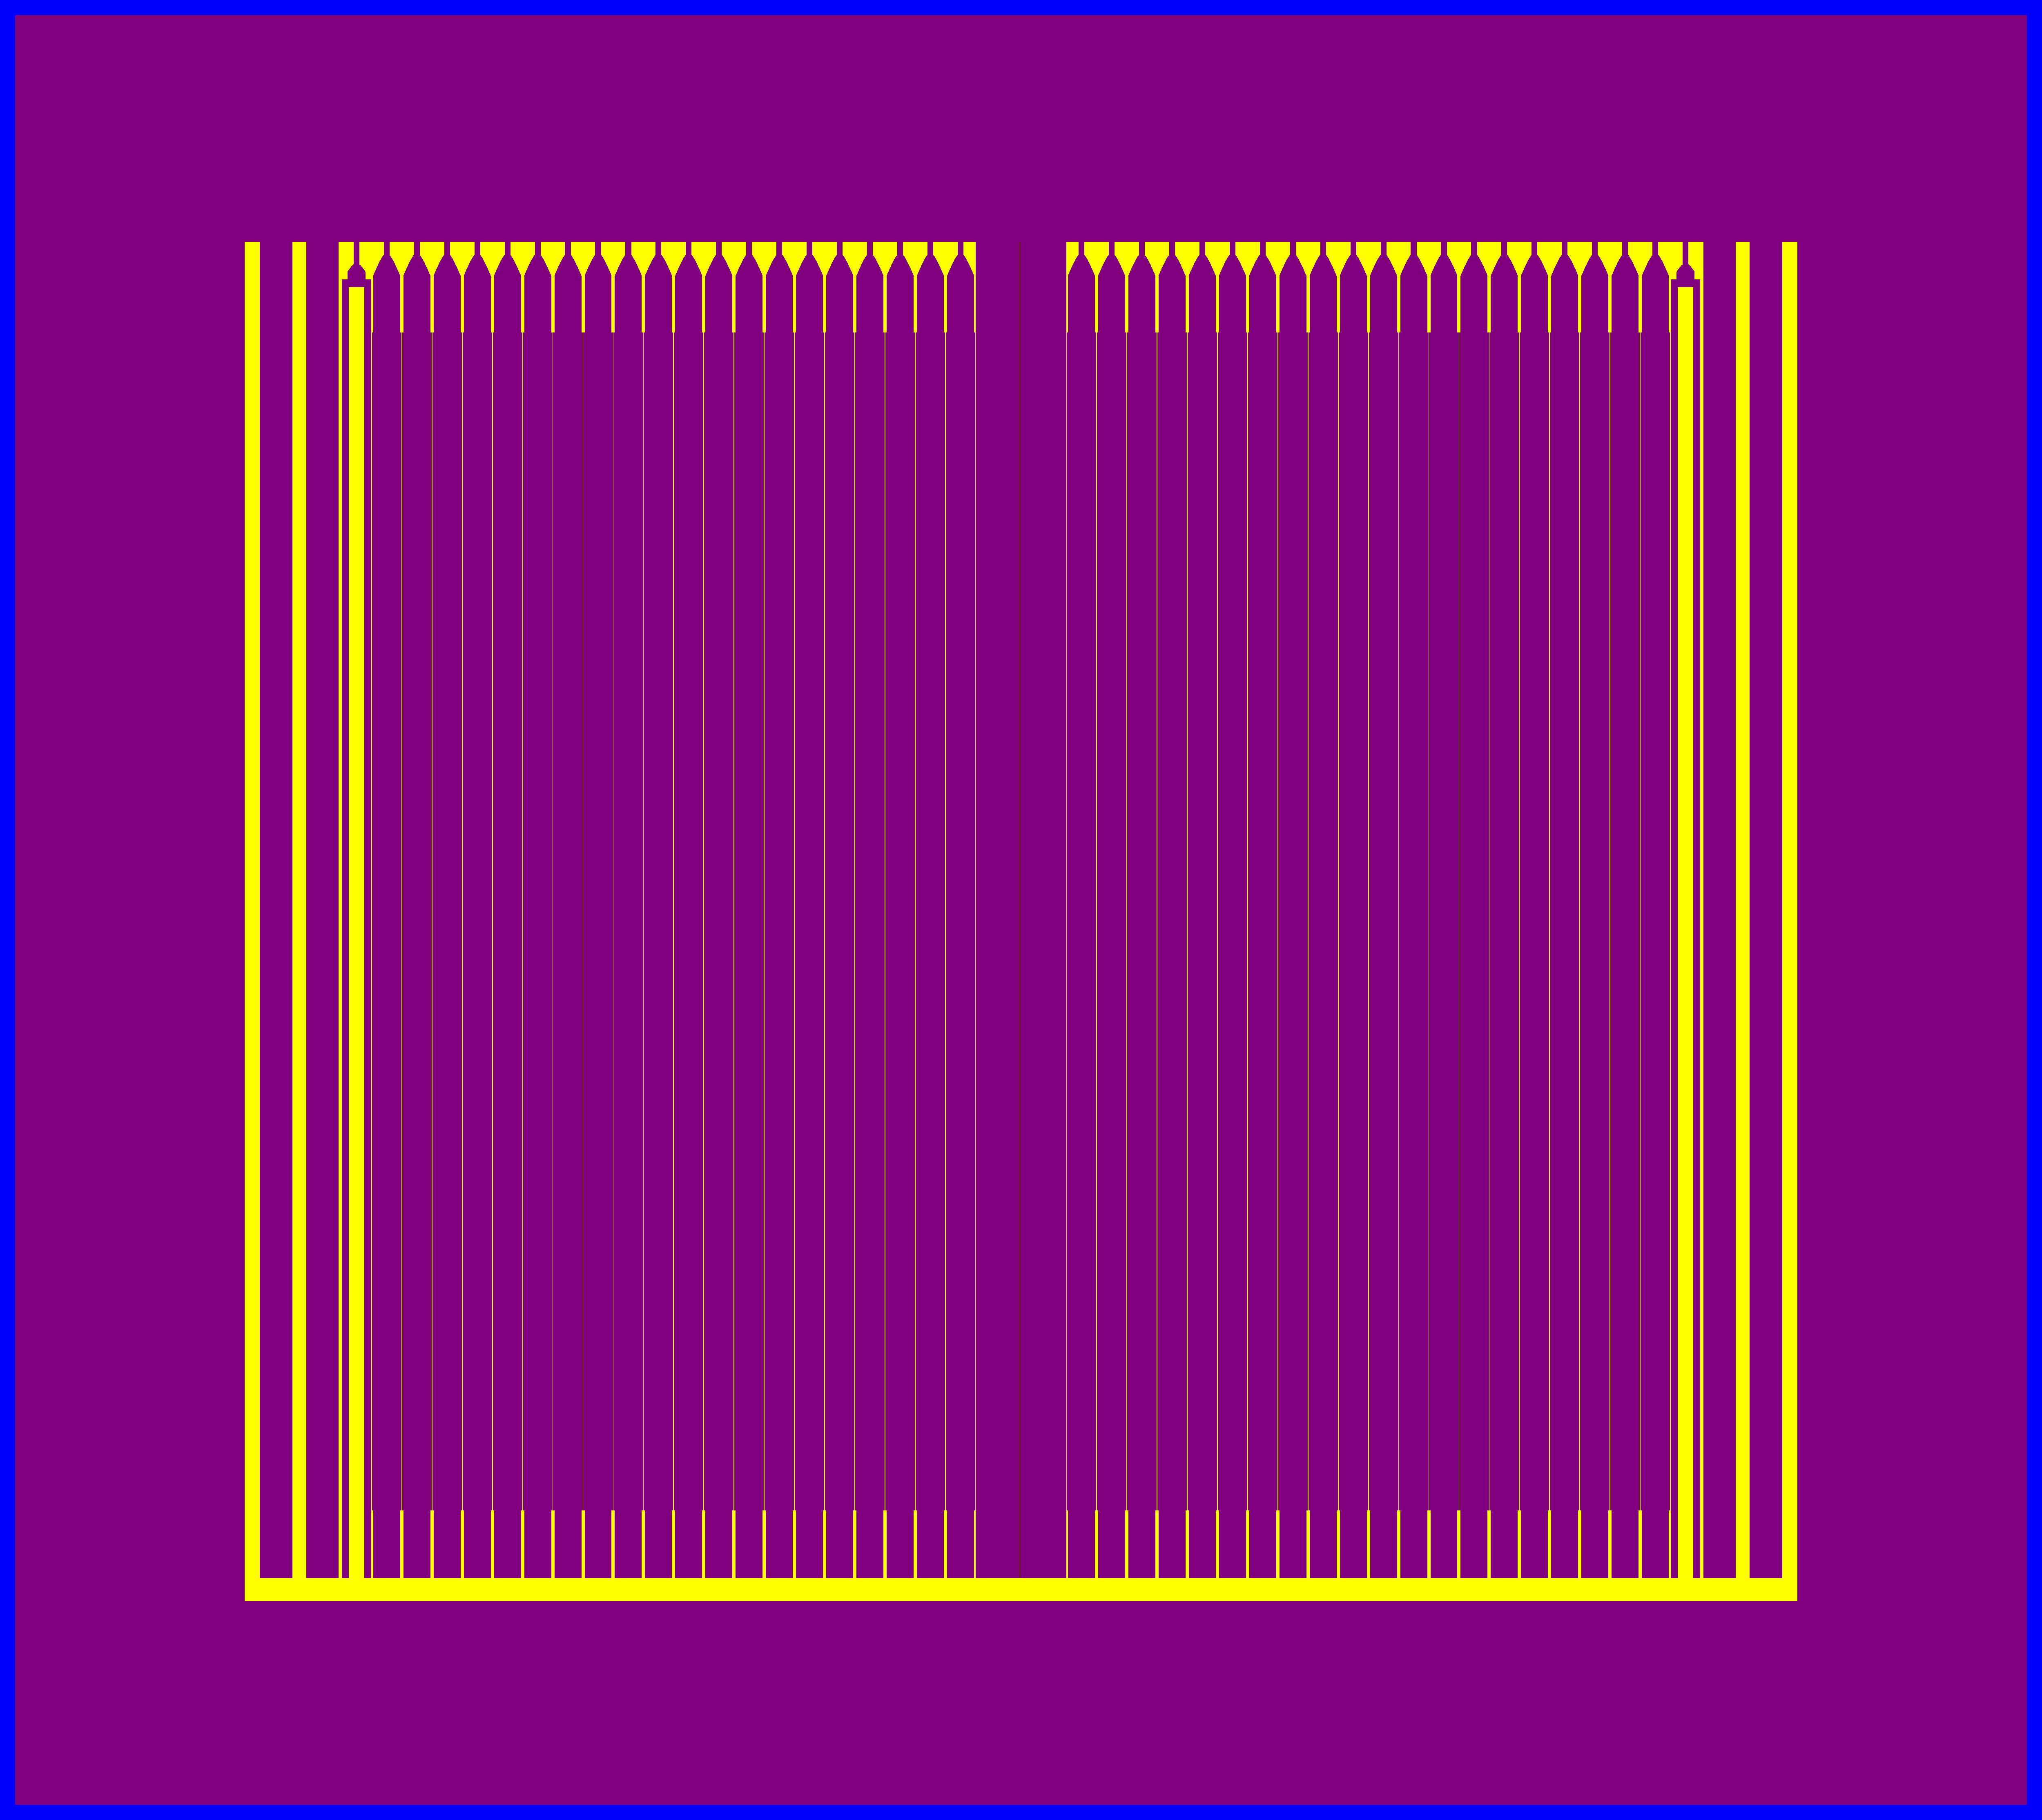
\includegraphics[width=0.5\linewidth]{figs/ch4/msbr_full_xz_openmc.png}
        \label{fig:msbr-model-xz}
    }
    \caption[Full views of MSBR]{
        \subref{fig:msbr-ref-xy} Top down view of \Gls{msbr} reference design.
        \subref{fig:msbr-model-xy} Top down view of \Gls{msbr} CSG model.
        \subref{fig:msbr-ref-xz} Side view of \Gls{msbr} reference design.
        \subref{fig:msbr-model-xz} Side view of \Gls{msbr} CSG model.
    }
    \label{fig:msbr-overview}
\end{figure}

As seen in Figure \ref{fig:msbr-overview}, the \Gls{csg} \Gls{msbr}
model reproduces these systems with several approximations. I will
describe each reactor system, as well as any relevant changes or
approximations made in the model.

\section{Materials}
\label{sec:msbr-materials}

\subsection{Fuel salt}
\label{sub:msbr-fuel-salt}
Table S.1 in \cite{robertson_conceptual_1971} specifies the fuel salt
composition used in the \Gls{msbr}:
\ce{LiF}-\ce{Be}\ce{F_2}-\ce{Th}\ce{F_4}-\ce{U}\ce{F_4} at a concentration of
71.7-16-12-0.3 mole-\%. The lithium used in the fuel salt is enriched to
99.995\% \ce{^{7}Li}. This is because \ce{^{6}Li} is a strong neutron absorber
and produces tritium in the absorption reaction. The atom-\% for each nuclide is
given in Table \ref{tab:msbr-fuel-salt-ref}\footnote{Most of the discussion of
the fuel salt composition in Robertson el al. (1971)
\cite{robertson_conceptual_1971}
specify elemental version of the nuclides in Table \ref{tab:msbr-fuel-salt-ref}.
I have specific specific nuclides for the following reasons: (1) both \ce{F} and
\ce{Be} have only one stable isotope, (2) the fuel salt receives initial fissile
loading from \ce{^{233}U} or \ce{^{235}U}, and (3) the fuel salt receives its
fertile loading from \ce{^{232}Th}}\footnote{I use OpenMC's Python API with the
ENDF/V VII.0 library along with a custom Python script
(\url{github.com/arfc/2022-yardas-ms/tree/master/model/salt-composition.ipynb})
to calculate these values. You may obtain slightly different numbers if you use
a different cross section library or calculation method, but they should  be
roughly the same.}.

See Section \ref{sec:salt-volume} for additional discussion of the value used
for the salt volume\footnote{I recommend reading this section after the geometry
description in Section \ref{sec:msbr-core}}

\begin{table}[htpb] 
    \centering 
    \caption{Reference \Gls{msbr} fuel salt specifications rounded to six decimals}
    \label{tab:msbr-fuel-salt-ref}
    \begin{tabular}{|c|c|c|c|c|c|c|} 
        \hline
        & \ce{^{6}Li} & \ce{^{7}Li} & \ce{^{19}F} & \ce{^{9}Be} & \ce{^{232}Th} & \ce{^{233}U}\\
        \hline 
        atom-\% & 1.315629 & 27.035498 & 60.458679 & 6.326611 & 4.744958 & 0.118624 \\
        \hline
        mass-\% & 0.312561 & 7.491697 & 45.366139 & 2.251942 & 43.485823 & 1.091838\\ 
        \hline
    \end{tabular}
\end{table}

The density of the fuel salt is given by a function\footnote{This function 
comes from an earlier report on the Molten-Salt Reactor Program
\cite{rosenthal_molten-salt_1969}.} of temperature in \unit{\celsius} in Table
S.1 in Robertson et al. (1971) \cite{robertson_conceptual_1971}:
\begin{equation}
    \rho = 3.752 - 6.68\cdot 10^{-4} \cdot T \quad \unit{\gram\per\cubic\centi\meter}
\end{equation}

The temperature of the fuel salt flowing into the core at the inlet at the
bottom of the reactor is 1050\unit{\degree}F (565.5556\unit{\celsius}, 838.7056
\unit{\kelvin}), and the temperature of the fuel salt flowing out of the core at
the outlet is approximately 1300\unit{\degree}F (704.4444\unit{\celsius},
977.5944 \unit{\kelvin}) \cite{robertson_conceptual_1971}. The average
temperature of the salt over the core inlets and outlets is then 1175
\unit{\degree}F (635\unit{\celsius}, 908.15 \unit{\kelvin}). While the
various solid components of the core are at a slightly higher temperature on
average\footnote{see figure 3.29 in \cite{robertson_conceptual_1971}}, for
simplicity, I set the evaluated temperature of all materials to 900
\unit{\kelvin} consistent cross-section selection between the \OpenMC and
\SerpentTWO depletion steps. At this temperature, the density of the fuel salt
is 3.3332642 \unit{\gram\per\centi\metre\cubed}.

\begin{table}[htpb] 
    \centering 
    \caption{Model \Gls{msbr} fuel salt specifications rounded to six decimals}
    \label{tab:msbr-fuel-salt-model}
    \begin{tabular}{|c|c|c|c|c|c|} 
        \hline
        & \ce{^{7}Li} & \ce{^{19}F} & \ce{^{9}Be} & \ce{^{232}Th} & \ce{^{233}U}\\
        \hline 
        atom-\% & 28.387735 & 60.435213 & 6.330366 & 4.747774 & 0.098912 \\
        \hline
        mass-\% & 7.875053& 45.398353 & 2.255754 & 43.559435 & 0.911405\\ 
        \hline
    \end{tabular}
\end{table}
% WILL NEED TO DO TEST SIMULATIONS TO CONFIRM THIS MATCHES PARK ET AL
In the CSG model, we use a mole-\% composition of 71.75-16-12-0.25. This slight
difference is due to an unpublished reactivity study investigating decreased
composition of \ce{UF_4} to obtain a more reasonable 
$k_\text{eff}$\footnote{According to Rykhlevskii, using 0.3 mole-\% \ce{UF_4} 
gave $k_\text{eff} > 1.3$} \cite{rykhlevskii_personal_2022}. The fuel salt 
material uses the composition specified in Table \ref{tab:msbr-fuel-salt-model}
and has a density of 3.35 \unit{\gram\per\centi\metre\cubed}. Notice that the
lithium has been enriched to 100\% \ce{^{7}Li}. This is because during initial
simulations, even those very small amounts of \ce{^{6}Li} were enough to kill
the reaction. The initial fissile and fertile loading has also been slightly
increased.

\subsection{Graphite}
\label{sub:graphite}

For a detailed description of the reactor graphite used in the \Gls{msbr}, see
Section 3.2.3 in \cite{robertson_conceptual_1971}. At 70\unit{\degree}F (294.3
\unit{\kelvin}), the \Gls{msbr} graphite has a density of 1843
\unit{\kilo\gram\per\cubic\metre}. This is the only density specification
for graphite that I was able to find in Robertson et al. (1971)
\cite{robertson_conceptual_1971}. In the CSG model, the graphite material uses
elemental carbon and has a density of 1.84 \unit{\gram\per\centi\metre\cubed}.

\subsection{Modified Hastelloy N}
\label{sub:hastelloy}
Hastelloy N is an alloy developed at \Gls{ornl} during the Molten-Salt Reactor
Program as a structural material that could maintain structural stability while
in contact with the corrosive and high temperature molten salt fuel while also
being under irradiation for a long period of time.

The \Gls{msbr} used a modified version of Hastelloy N designed to improve
embrittlement resistance and weldability \cite{robertson_conceptual_1971}.
The \Gls{msbr} uses modified Hastelloy N on all nearly all salt-facing
components included in the CSG model.

Modified Hastelloy N has a density of 8671 \unit{\kilo\gram\per\cubic\metre} at
1300\unit{\degree}F (704.4444\unit{\celsius}, 977.5944 \unit{\kelvin})
\cite{robertson_conceptual_1971}. The elemental composition of modified
Hastelloy N and their amounts in mass-\% are in Table \ref{tab:hastelloy-n-ref}.

\begin{table}[htpb]
    \centering
    \caption[Mass-\% of elements in modified Hastelloy N used in the \Gls{msbr}]{Mass-\% of elements in modified Hastelloy N used in the \Gls{msbr}. Data from Table 3.1 and S.1 in \cite{robertson_conceptual_1971}. Ranged values collapsed to their average are denoted with a $^*$}
    \label{tab:hastelloy-n-ref}
    \begin{tabular}{|c|c|c|c|c|c|c|c|c|c|c|c|c|c|c|c|c|}
        \hline
        \ce{Ni} & \ce{Mo}$^*$ & \ce{Cr}$^*$ & \ce{Fe}$^*$ & \ce{C}$^*$ & \ce{Mn}$^*$ & \ce{Si} & \ce{W} & \ce{Al} & \ce{Ti}$^*$ & \ce{Cu} & \ce{Co} & \ce{P} & \ce{S} & \ce{B} & \ce{Hf}$^*$ & \ce{Nb}$^*$ \\
        \hline
        73.709 & 12 & 7 & 3 & 0.06 & 0.35 & 0.1 & 0.1 & 0.1 & 1.25 & 0.1 & 0.2 & 0.015 & 0.015 & 0.001 & 1 & 1\\
        %\hline
        %atom-\% & 76.72 & 7.64 & 8.224 & 3.282 & 0.305 & 0.389 & 0.218 & 0.033 & 0.226 & 1.595 & 0.096 & 0.207 & 0.03 & 0.029 & 0.006 & 0.342 & 0.658 \\
        \hline
    \end{tabular}
\end{table}

\begin{table}[htpb]
    \centering
    \caption{Mass-\% of elements in modified Hastelloy N used in the \Gls{msbr} model.}
    \label{tab:hastelloy-n-model}
    \begin{tabular}{|c|c|c|c|}
        \hline
        \ce{Ni} & \ce{Cr} & \ce{W} & \ce{Al} \\
        \hline
        67.7 & 7.0 & 25.0 & 0.3 \\
        \hline
    \end{tabular}
\end{table}

The Hastelloy N material in the CSG model uses the composition specified in
Table \ref{tab:hastelloy-n-model} and has a density of 8.671 
\unit{\gram\per\centi\metre\cubed}. The model material has a different
composition than the reference material because the additional elements are of
little neutronic importance  and their omission reduces computation time
according to Rykhlevskii \cite{rykhlevskii_personal_2022}.


\section{Reactor core}
\label{sec:msbr-core}
The \Gls{msbr} core is split into three distinct different zones; zone I, zone
II, and the reflector zone. 

\begin{figure}[htpb]
    \centering
    \subfloat[][]{
        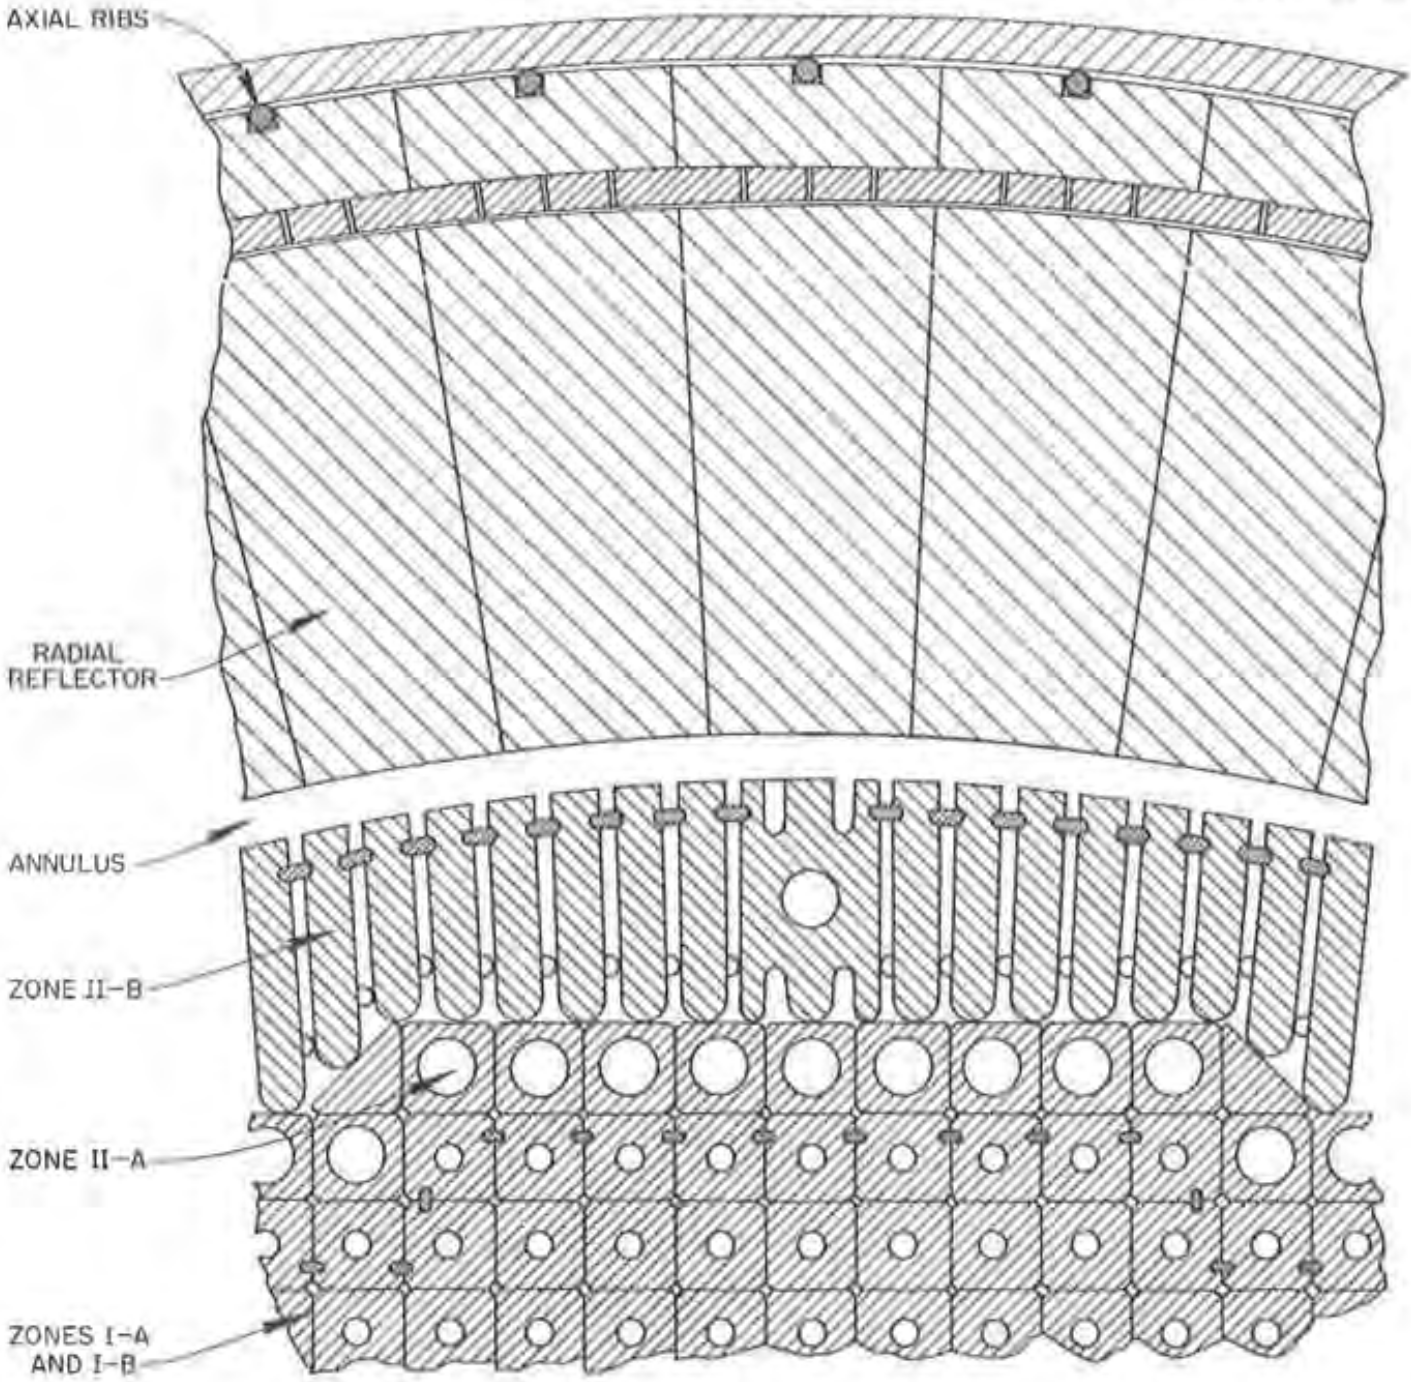
\includegraphics[width=0.45\linewidth]{figs/ch4/msbr_section_ref.png}
        \label{fig:msbr_sec_ref}
    }
    \subfloat[][]{
        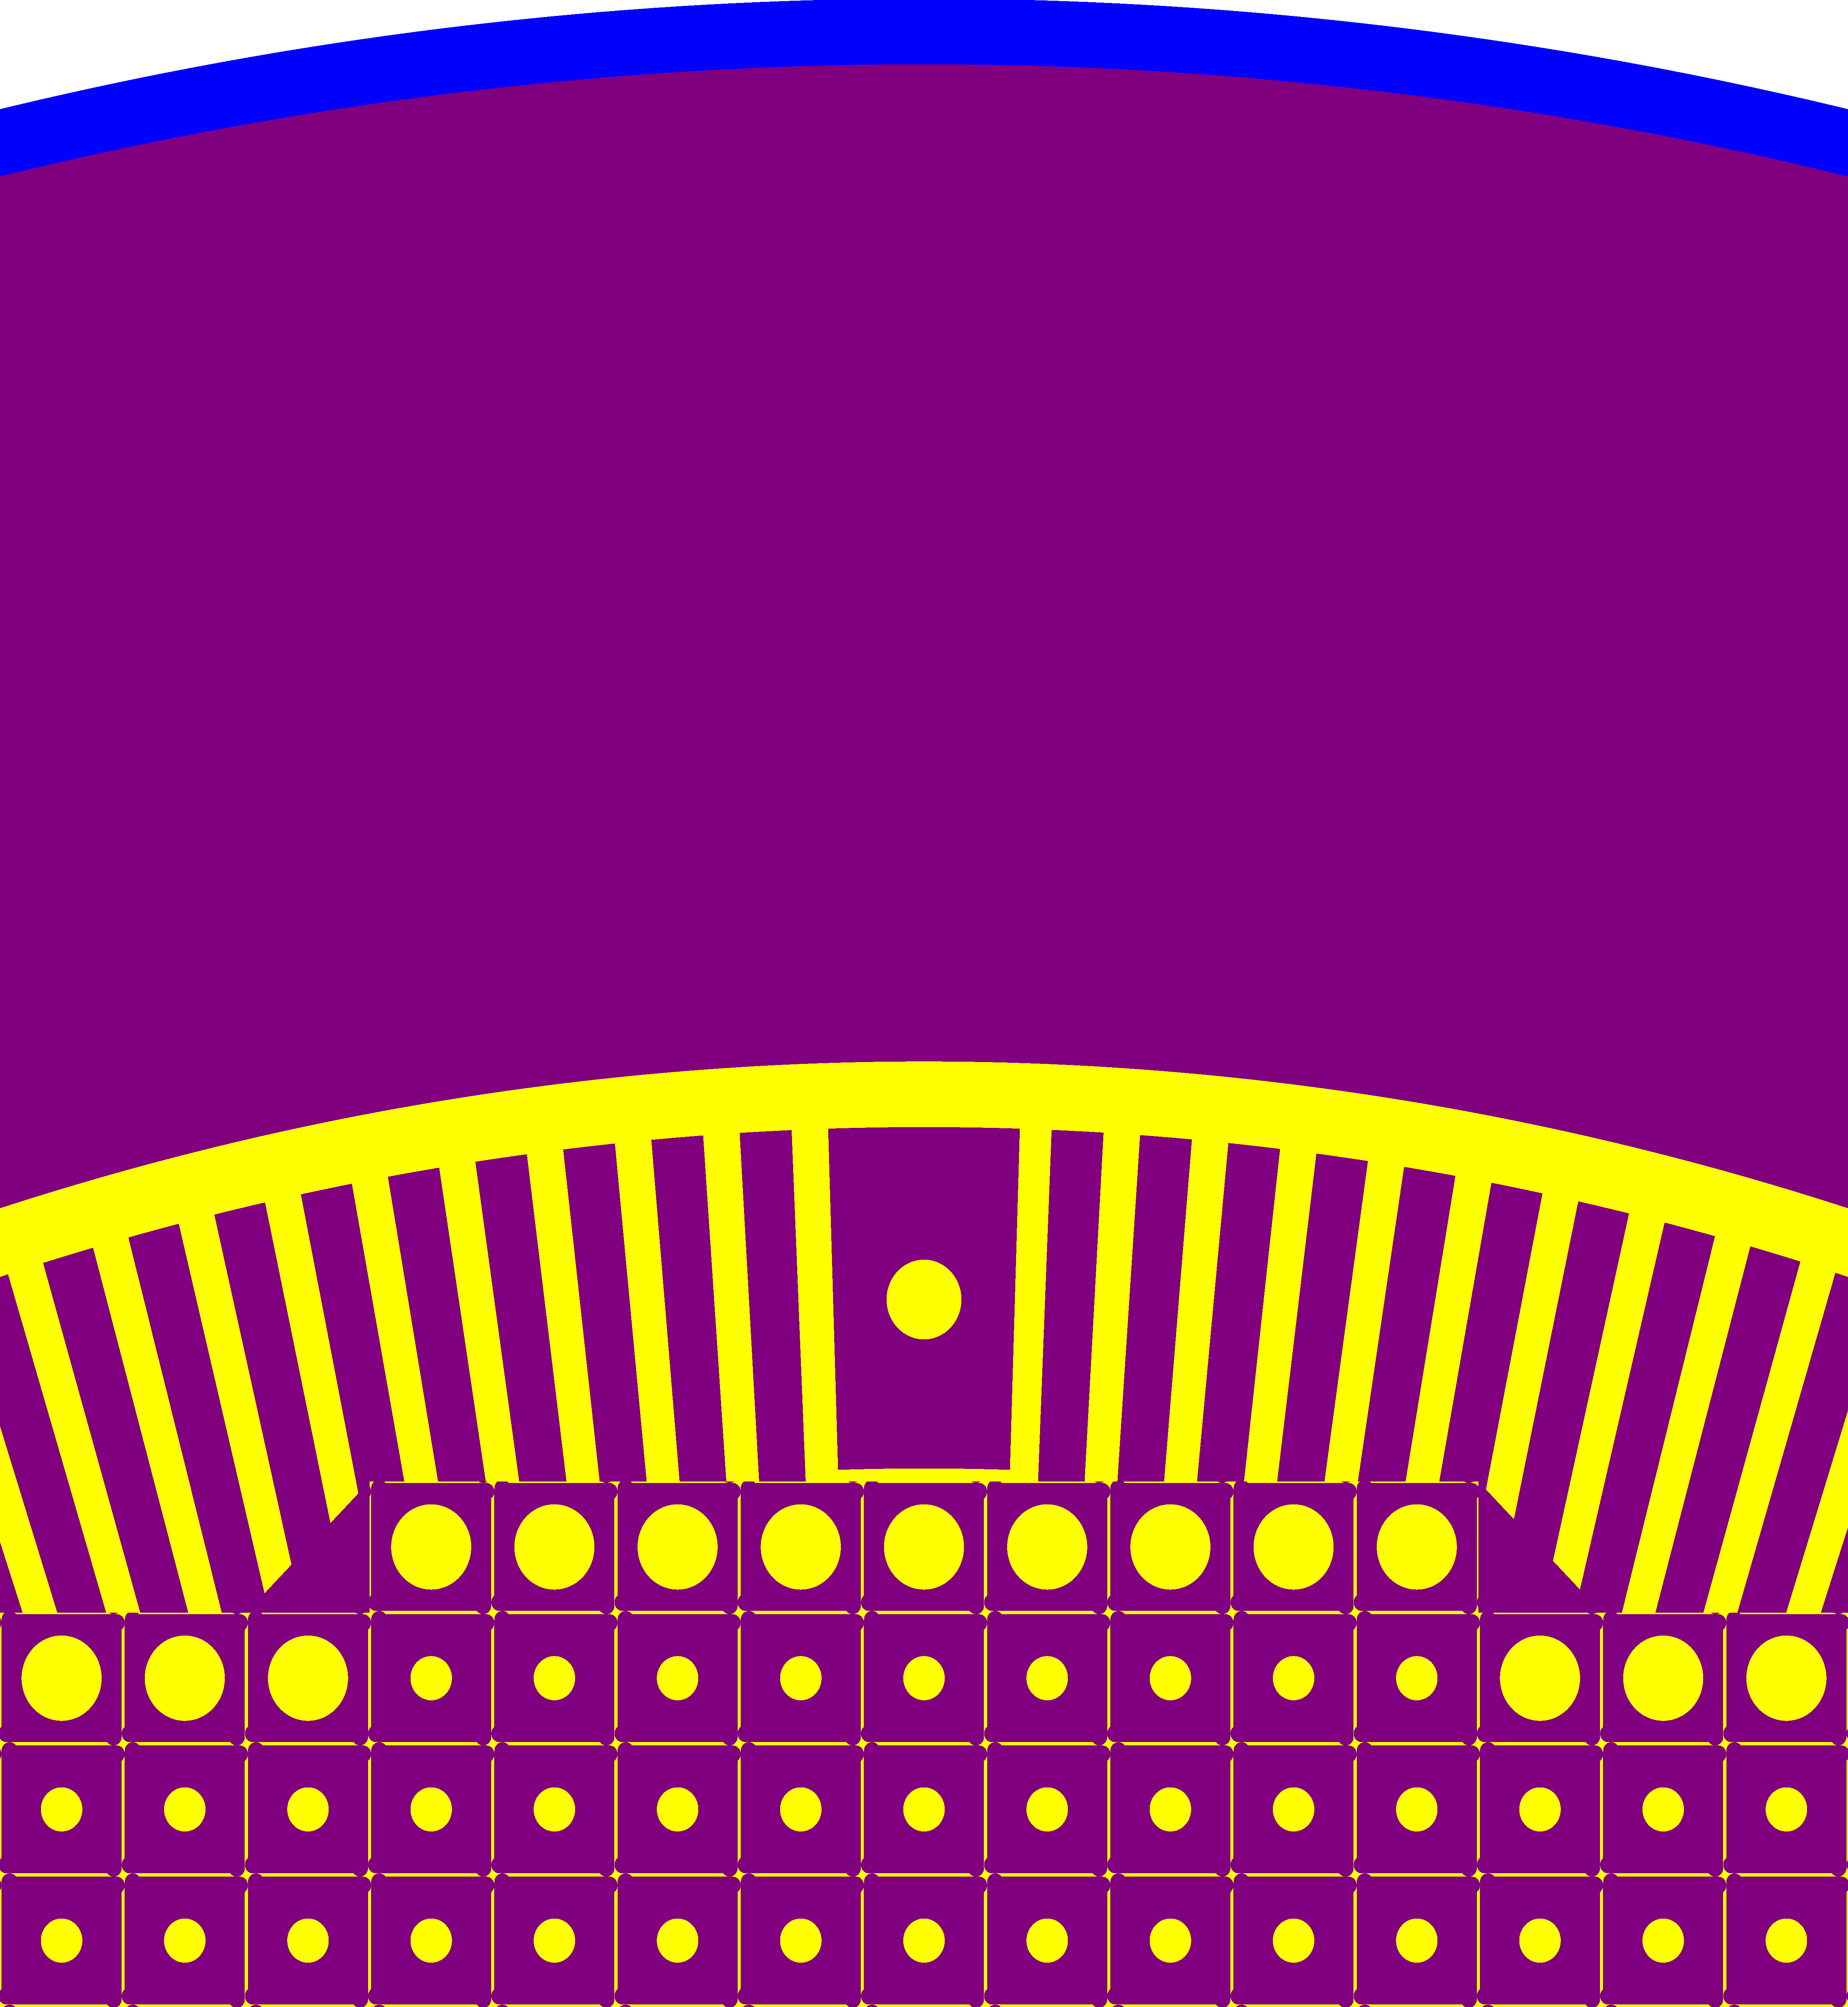
\includegraphics[width=0.35\linewidth]{figs/ch4/msbr_section_openmc.png}
        \label{fig:msbr_sec_model}
    }
    \caption[Detail views of MSBR core region]{
        \subref{fig:msbr_sec_ref} Detail view of \Gls{msbr} reference design.
        \subref{fig:msbr_sec_model} Detail view of \Gls{msbr} CSG model.}
    \label{fig:msbr-detail}
\end{figure}

\subsection{Zone I} Zone I is the central-most region of the core, and is 13.2\%
fuel salt by volume. Zone I is divided into three subzones: zone I-A, zone I-B,
and the control rod zone.

Zone I-A and I-B consist of 4 in. $\times$ 4 in. (10.16 cm $\times$ 10.16 cm)
square graphite elements. As seen in Figures \ref{fig:msbr-ia-xy} and
\ref{fig:msbr-ib-xy}, elements in both zones have axial ribs protruding from
the faces of the square elements near the corners, as well as cylindrical
channels in the centers of the elements. The purpose of the fuel holes are to
facilitate salt flow through the core elements. The purpose of the ribs are to
separate the elements from each other as well as create interstitial salt flow
channels \cite{robertson_conceptual_1971}. These interstitial flow channels
are seen in Figures \ref{fig:msbr-ia-lattice} and
\ref{fig:msbr-ib-lattice}\footnote{Notice that the shape of the model zone I-B
elements qualitatively matches the reference design in Figure
\ref{fig:msbr-ib-xy}, but  not in Figure \ref{fig:msbr-ib-lattice}, despite
matching nearly all specifications of the reference design.}.

The only dimensional differences between the zone I-A and I-B elements are the
diameter of the cylindrical fuel channels and the size of the axial ribs (see
Tables \ref{tab:zone-ia-ref-specs} and \ref{tab:zone-ib-specs}). Zone I-A
elements have a smaller cylindrical channel and larger interstitial channel
than zone I-B elements. The central part of zone I consists of zone I-A
elements, whereas the outer part of zone I consists of zone I-B
elements \cite{robertson_conceptual_1971}. The purpose this configuration is to
reduce the temperature gradient across the core. The salt velocity through the
zone I-B elemets is much lower than the salt velocity through the zone I-A
elements\footnote{Robetson et al. (1971) states that the salt velocity varies
``from 8 fps at the center [of the core] to about 2 fps near the periphery''
\cite{robertson_conceptual_1971}}.

Additionally the zone I elements are machined to a cylindrical shape at the ends
to create an undermoderated region of 37\% salt at the top and bottom of the
reactor \cite{robertson_conceptual_1971}. These machined ends are referred to as
Section A (see Figures \ref{fig:msbr-ia-xy}, \ref{fig:msbr-ib-xy}, and
\ref{fig:msbr-i-xz-full}). The top of each element also has an outlet plenum to
direct salt flow towards the exit nozzles at the edge of the vessel, however
these are not included in the \Gls{csg} model. The outermost layer of zone I
elements also have grooves in them to fit eliptical graphite sealing rods (see
Figure \ref{fig:msbr-detail}) that separate the salt flow in zone I from the
salt flow in zone II \cite{robertson_conceptual_1971}. Robertson et al. (1971)
does not specify precise dimensions and positions of these rods, so they are not
included in the \Gls{csg} model.

Robertson et al. (1971) does not specify exact distribution of zone I-A and I-B
elements. Rather than guess the distribution of I-A and I-B elements, the CSG
model assumes that zone I consists entirely of I-B elements. This assumption
greatly simplifies the work needed to create the model. Had we picked zone I-A
elements, we would have needed to create at least eight different ``versions''
of both the I-A elements and the II-A elements\footnote{four versions of each
element for each configuration where a I-A and II-A element are adjacent,
four versions of I-A elements for each configuration where the element is
adjacent to two II-A elements, and four versions of II-A elements for each for
configuration where the II-A element is adjacent to two I-A elements.}

\begin{table}[htpb]
    \centering
    \caption{Reference Zone I-A dimensions}
    \label{tab:zone-ia-ref-specs}
    \begin{tabulary}{\linewidth}{|C|C|C|}
    \hline
    Quantity & Dimension [in] & Dimension [\unit{\centi\metre}]\\
    \hline
    Section A inner diameter & 0.6 & 1.524 \\
    \hline
    Section A outer diameter & 3.698 & 9.39292 \\
    \hline
    Rib tip radius of curvature & 0.25 & 0.635 \\
    \hline
    Rib tip to element spacing & 0.302 & 0.76708 \\
    \hline
    Rib tip to element center & 1.315 & 3.3401 \\
    \hline
    Zone A height (bottom) & 9 & 22.86\\
    \hline
    Zone B height & 156 & 396.24 \\
    \hline
    Zone A height (top) & 7.5 & 19.05 \\
    \hline
    Conical part height & 2.75 & 6.985 \\
    \hline
    Hastelloy plug height & 2.875 & 7.3025 \\
    \hline
    Hastelloy plug diameter & 0.6 & 1.524 \\
    \hline
    Top part height & 1.75 & 4.445 \\
    \hline
    Top part outer diameter & 1.75 & 4.445 \\
    \hline
    \end{tabulary}
\end{table}


\begin{table}[htpb]
    \centering
    \caption{Zone I-B dimensions}
    \begin{tabulary}{\linewidth}{|C|CC|CC|}
    \hline
    Quantity & Reference Dimension [in] & Reference Dimension [\unit{\centi\metre}] & Model Dimension [in] & Model Dimension [\unit{\centi\metre}]\\
    \hline
    Section A inner diameter & 1.340 (Fig. \ref{fig:msbr_ib_bottom_ref}) or 1.347 (Fig. \ref{fig:msbr_ib_lattice_ref}) & 3.4036 or 3.42138 & 1.347 & 3.42138 \\
    \hline
    Section A outer diameter & 3.900 & 9.906 & 3.900 & 9.906 \\
    \hline
    Rib tip radius of curvature & 0.25 & 0.635 & 0.263 & 0.66802\\
    \hline
    Rib tip to element spacing & 0.1 & 0.254 & 0.1 & 0.254\\
    \hline
    Rib tip to element center & 1.687 & 4.28498 & 1.687 & 4.28498\\
    \hline
    Zone A height (bottom) & 9 & 22.86 & 9 & 22.86\\
    \hline
    Zone B height & 156 & 396.24 & 156 & 396.24\\
    \hline
    Zone A height (top) & 7.5 & 19.05 & 7.5 & 19.05\\
    \hline
    Conical part height & 2.75 & 6.985 & 2.75 & 6.985\\
    \hline
    Hastelloy plug height & 2.875 & 7.3025 & 1.75 & 4.445 \\
    \hline
    Hastelloy plug diameter & 1.340 (Fig. \ref{fig:msbr_ib_bottom_ref}) or 1.347 (Fig. \ref{fig:msbr_ib_lattice_ref}) & 3.4036 or 3.42138 & 1.347 & 3.42138 \\
    \hline
    Top part height & 1.75 & 4.445 & 1.75 & 4.445 \\
    \hline
    Top part outer diameter & 1.75 & 4.445 & 1.75 & 4.445\\
    \hline
    \end{tabulary}
\end{table}


\begin{figure}[htpb]
    \centering
    \subfloat[][]{
        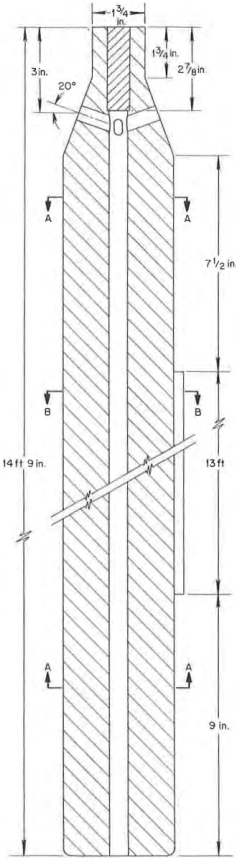
\includegraphics[width=0.25\linewidth]{figs/ch4/zone_i_full_ref.png}
        \label{fig:msbr_i_full_ref}
    }
    \subfloat[][]{
        
\includegraphics[width=0.17\linewidth]{figs/ch4/zone_ib_full_openmc.png}
        \label{fig:msbr_ib_full_model}
    }
    %\end{tabular}
    \caption[$xz$ cross sections of Zone I elements]{
        \subref{fig:msbr_i_full_ref} Reference zone I element
        \subref{fig:msbr_ib_full_model} Model zone I-B element
    }
    \label{fig:msbr-i-xz-full}
\end{figure}

\begin{figure}[htpb]
    \centering
    \subfloat[][]{
        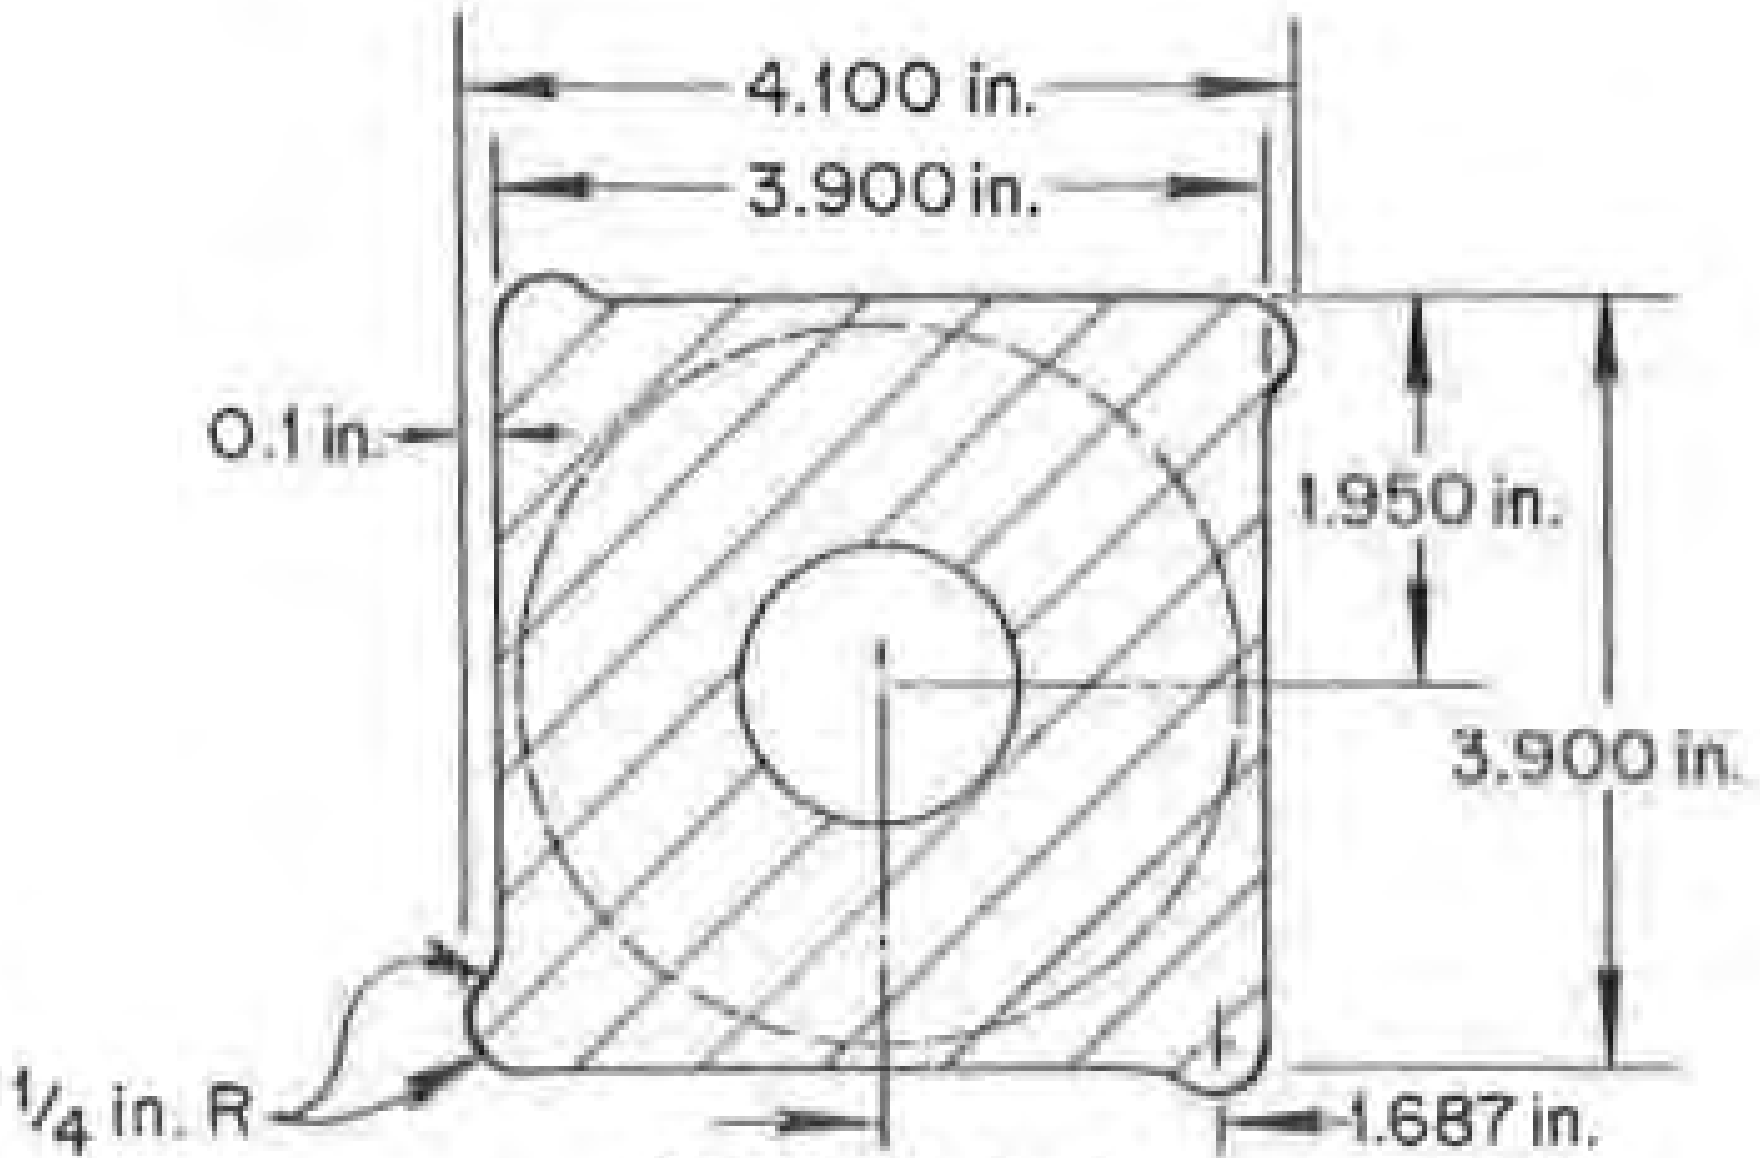
\includegraphics[width=0.3\linewidth]{figs/ch4/zone_ib_main_ref.png}
        \label{fig:msbr_ib_main_ref}
    }
    \subfloat[][]{
        
\includegraphics[width=0.2\linewidth]{figs/ch4/zone_ib_main_openmc.png}
        \label{fig:msbr_ib_main_model}
    }
    \\
    \subfloat[][]{
        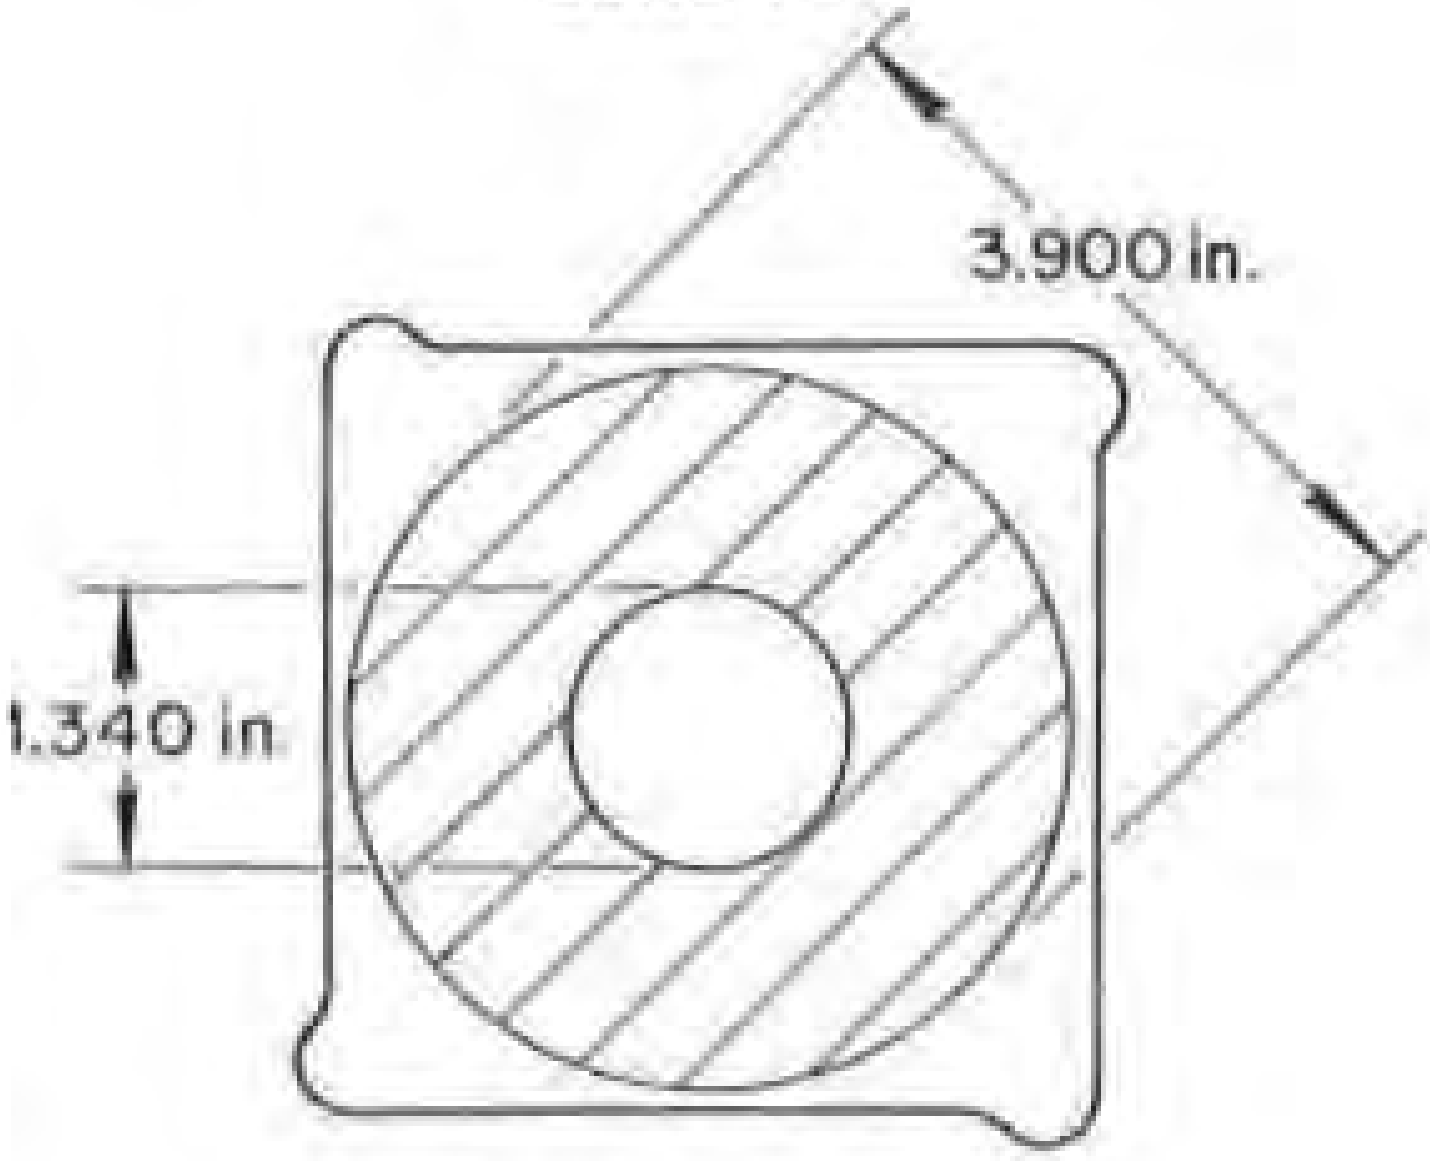
\includegraphics[width=0.3\linewidth]{figs/ch4/zone_ib_bottom_ref.png}
        \label{fig:msbr_ib_bottom_ref}
    }
    \subfloat[][]{
        
\includegraphics[width=0.2\linewidth]{figs/ch4/zone_ib_bottom_openmc.png}
        \label{fig:msbr_ib_bottom_model}
    }
    \caption[$xy$ cross sections of Zone I-B elements]{
        \subref{fig:msbr_ib_main_ref} Reference zone I-B element; section B.
        \subref{fig:msbr_ib_main_model} Model zone I-B element; section B.
        \subref{fig:msbr_ib_bottom_ref} Reference zone I-B element; section A.
        \subref{fig:msbr_ib_bottom_model} Model zone I-B element; section A.
    }
    \label{fig:msbr-ib-xy}
\end{figure}

\begin{figure}[htpb]
    \centering
    \subfloat[][]{
        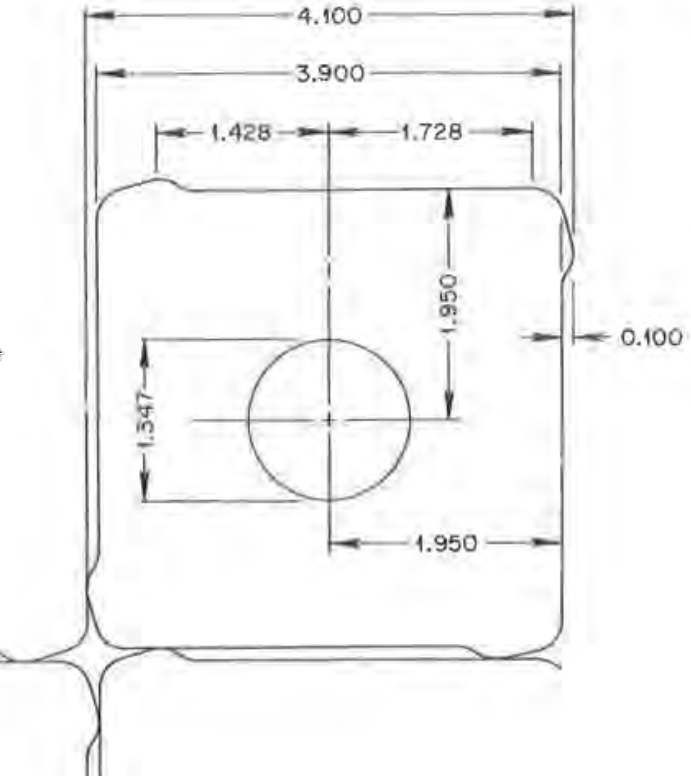
\includegraphics[width=0.25\linewidth]{figs/ch4/zone_ib_lattice_ref.png}
        \label{fig:msbr_ib_lattice_ref}
    }
    \subfloat[][]{
        
\includegraphics[width=0.17\linewidth]{figs/ch4/zone_ib_lattice_openmc.png}
        \label{fig:msbr_ib_lattice_model}
    }
    %\end{tabular}
    \caption[Lattice view of Zone I-B elements]{
        \subref{fig:msbr_ib_lattice_ref} Reference zone I-B lattice
        \subref{fig:msbr_ib_lattice_model} Model zone I-B lattice 
    }
    \label{fig:msbr-ib-lattice}
\end{figure}


\begin{figure}[htpb]
    \centering
    \subfloat[][]{
        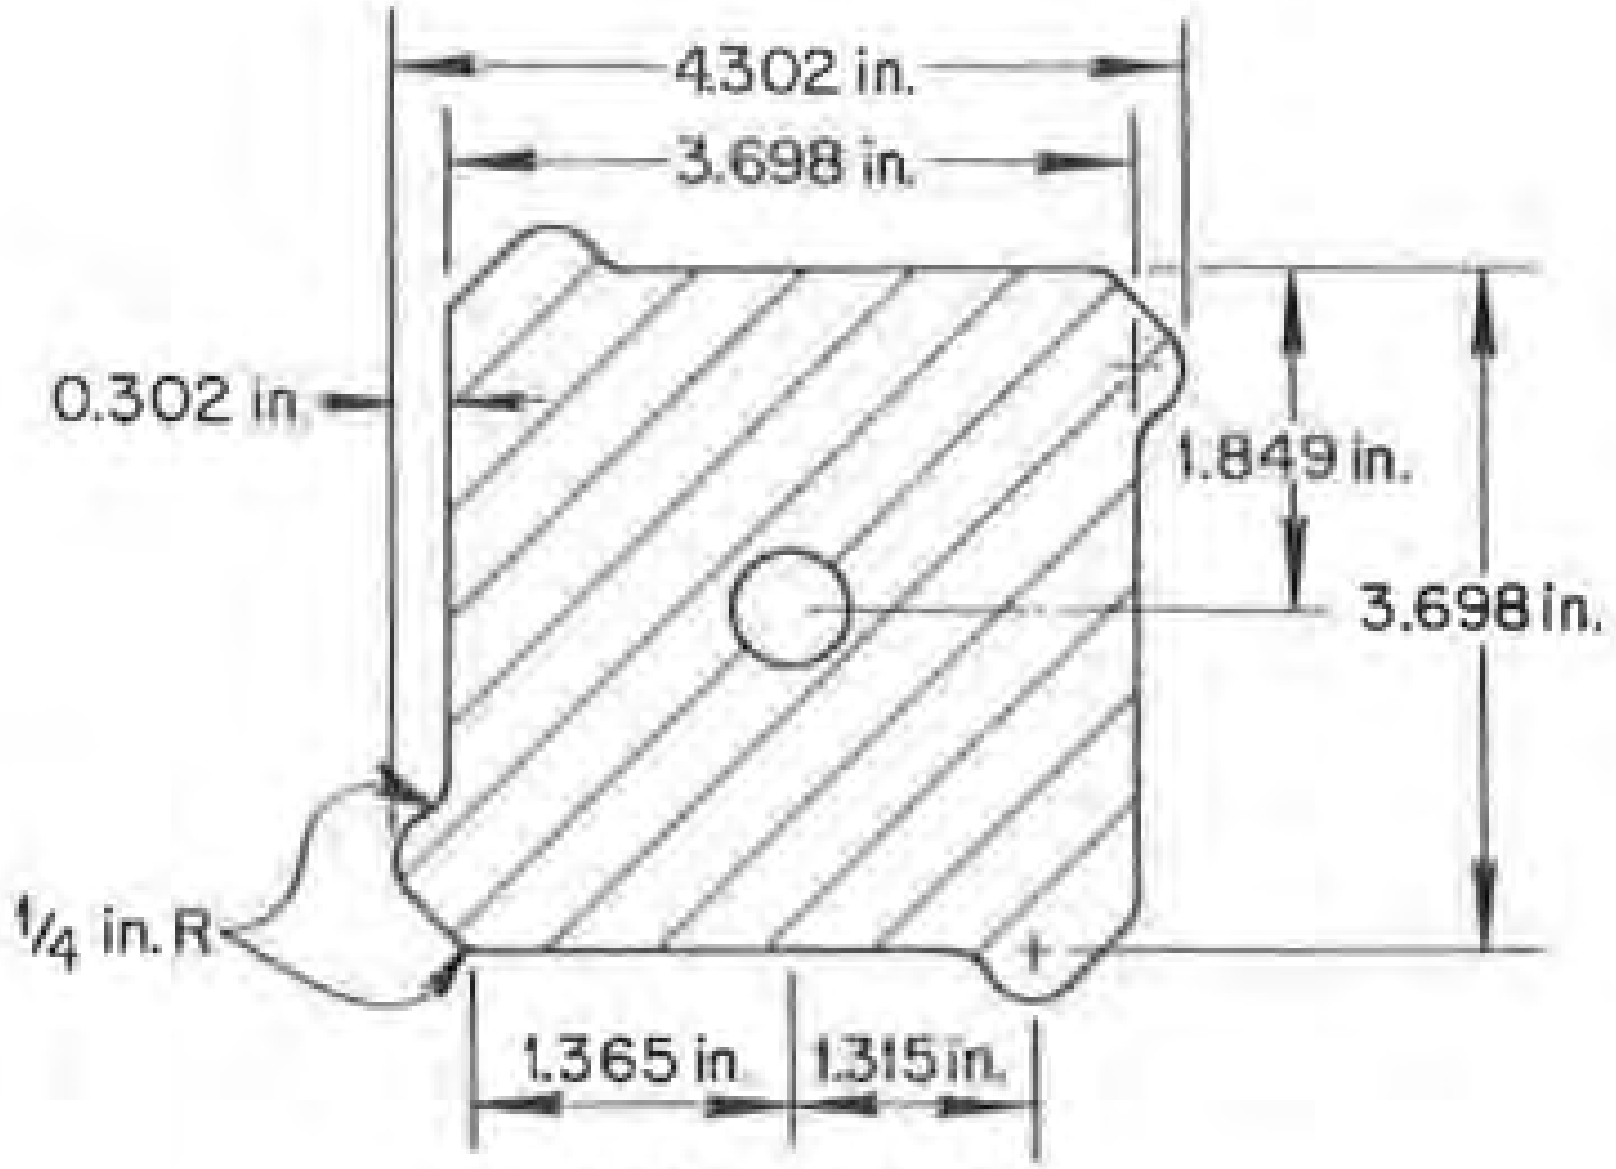
\includegraphics[width=0.3\linewidth]{figs/ch4/zone_ia_main_ref.png}
        \label{fig:msbr_ia_main_ref}
    }
    \subfloat[][]{
        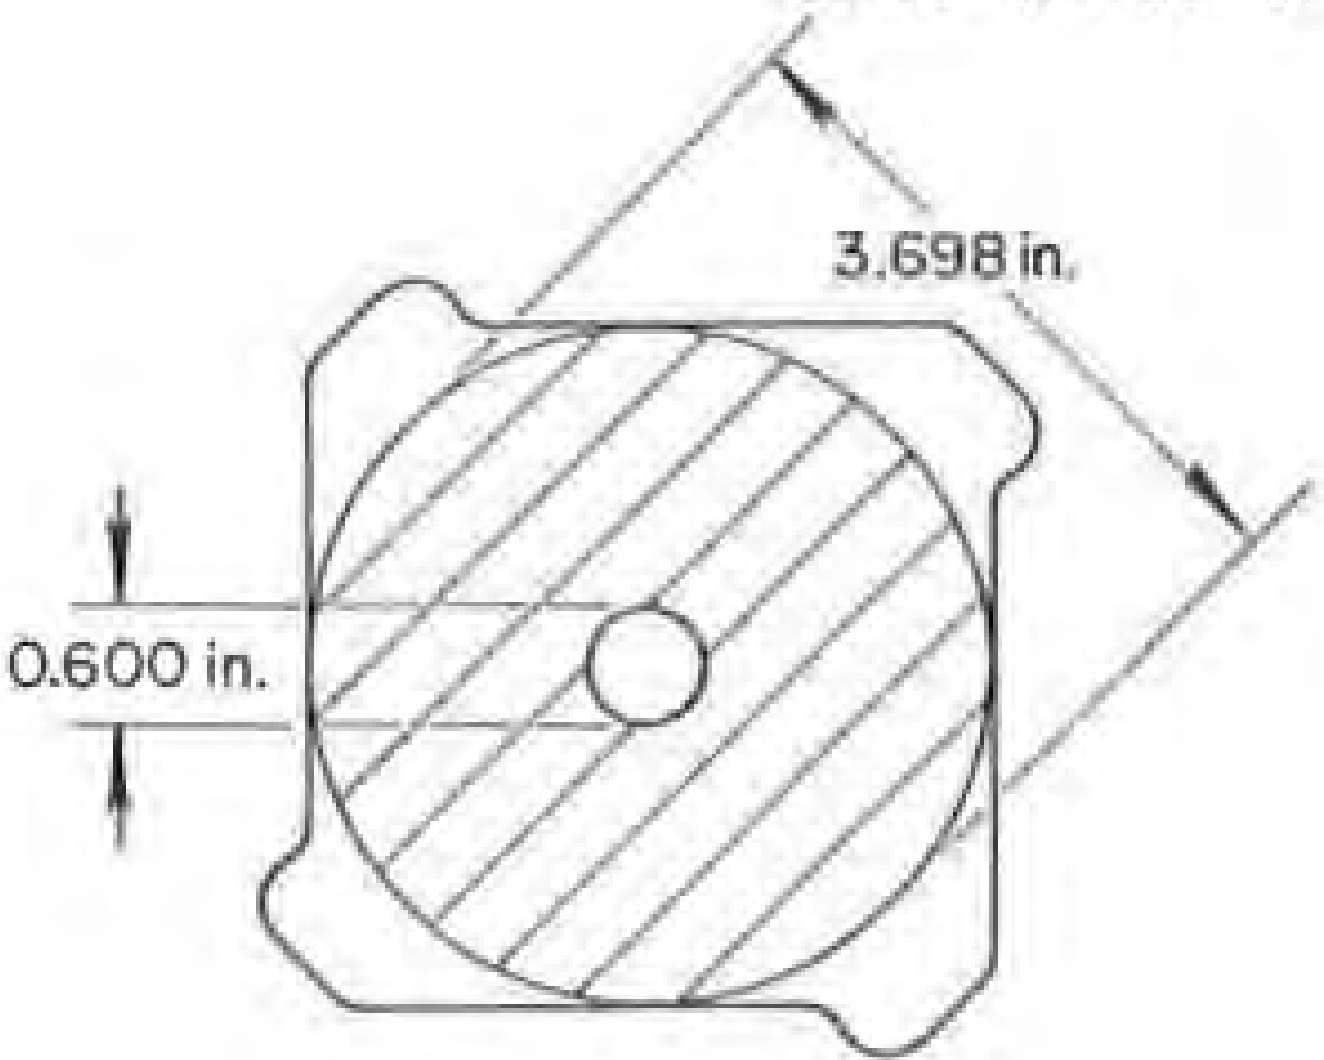
\includegraphics[width=0.3\linewidth]{figs/ch4/zone_ia_bottom_ref.png}
        \label{fig:msbr_ia_bottom_ref}
    }
    \caption[$xy$ cross sections of Zone I-A elements]{
        \subref{fig:msbr_ia_main_ref} Reference zone I-A element; Section B.
        \subref{fig:msbr_ia_bottom_ref} Reference zone I-A element; Section A.
    }
    \label{fig:msbr-ia-xy}
\end{figure}

\begin{figure}[htpb]
    \centering
    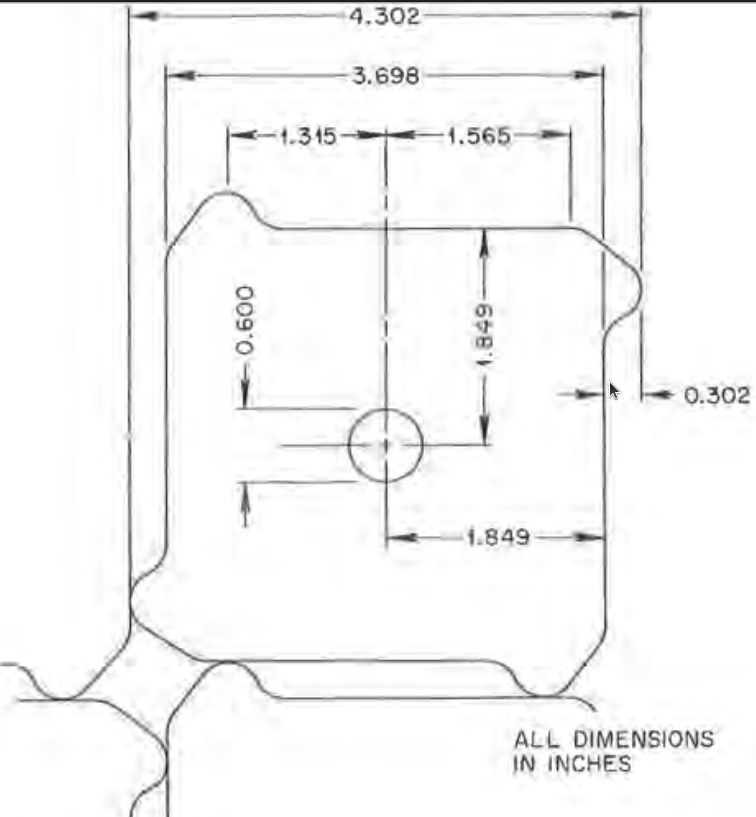
\includegraphics[width=0.25\linewidth]{figs/ch4/zone_ia_lattice_ref.png}
    \caption{Lattice view of zone I-A elements}
    \label{fig:msbr-ia-lattice}
\end{figure}

Four 6 in. $\times$ 6 in.
(15.24-cm $\times$ 15.24-cm) graphite elements
sit at the center of the core. Two of these elements contain graphite control
rods, and the other two elements are for neutron-absorbing rods for shutting
down the reactor, and are left empty during operation
\cite{robertson_conceptual_1971}. Robertson el al does not specify a design nor
dimensions for the control rod graphite elements. The \Gls{csg} model assumes
that these elements will be similar in shape to the zone I-A element (see Table
\ref{tab:cr-specification} and Figure \ref{fig:control-rods}). The control rods
themselves have axial passages through them to facilitate salt flow, but the
dimensions of these passages are not given, so the \Gls{csg} model does not
include them.

\begin{table}[htpb]
    \centering
    \caption{Control rod specifications}
    \label{tab:cr-specification}
    \begin{tabulary}{\linewidth}{|C|CC|CC|}
        \hline
        Quantity & Reference Dimension [in] & Reference Dimension [\unit{\centi\metre}] & Model Dimension [in] & Model Dimension [\unit{\centi\metre}]\\
        \hline
        Control rod element side length & 6 & 15.24 & 5.698 & 14.47292 \\
        \hline
        Control rod element inner diameter & 4 & 10.16 & 4 & 10.16\\
        \hline
        Control rod diameter & 3.75 & 9.525 & 3.75 & 9.525 \\
        \hline
        Rib tip radius of curvature & -  & - & 0.3897638 & 0.99\\
        \hline
        Rib tip to element spacing & - & - & 0.302 & 0.76708 \\
        \hline
        Rib tip to element center & - & - & 3.151 & 8.00354\\
        \hline
    \end{tabulary}
\end{table}

\begin{figure}[htpb]
    \centering
    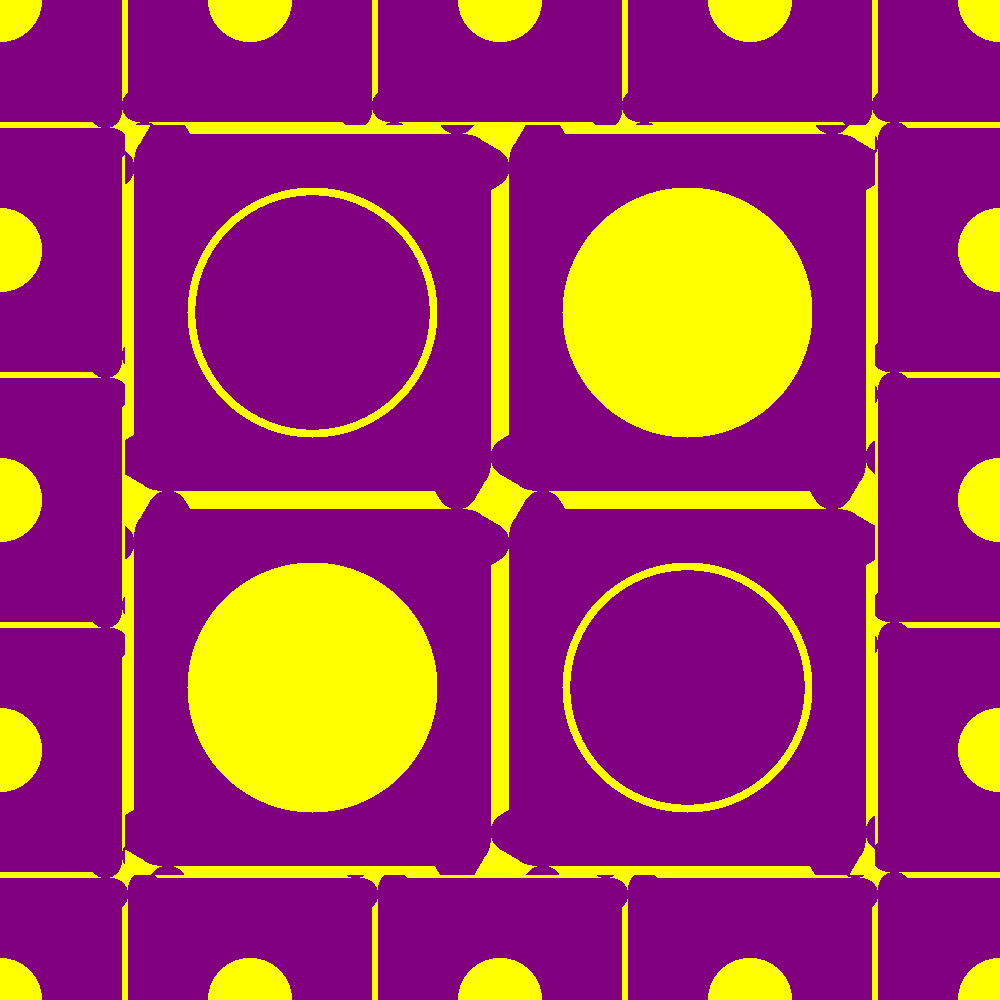
\includegraphics[width=0.5\textwidth]{figs/ch4/cr_xy_openmc.png}
    \caption{CSG model control rod lattice}
    \label{fig:control-rods}
\end{figure}


\subsection{Zone II}

Zone II is the undermoderated zone surrounding zone I, and is 37\% fuel salt by
volume. Zone II acts as a blanket zone that reduces neutron leakage from the
core \cite{robertson_conceptual_1971}. Zone II is divided into two subzones: zone
II-A and zone II-B.

Zone II-A consists of elements that are identical to zone I-B elements except
that their cylindrical fuel channel is larger, there is no machining on the bottom part of the elements, and the machining on the top part of the elements is different. (see Table \ref{tab:zone-iia-specs} and Figures \ref{fig:msbr-iia-xz-full} and \ref{fig:msbr-iia-xy}). Half-square triangular graphite elements of the same dimension as the zone II-A elements are present at lattice cells where there would be a nothing connecting zone II-A elements (see Figure \ref{fig:msbr-detail}). 

Zone II-B consists of two different types of elements arranged radially around the core: eight 6 in. (15.24 \unit{\centi\metre}) wide 13 ft. (396.24 \unit{\centi\metre}) tall rectangular slats with holes to fit the 2.5 in. diameter core lifting rods\footnote{the diameter of these holes is unknown, so the \Gls{csg} model assumes they are 6.176 cm in diameter} arranged at 45\unit{\degree} intervals, and 200 (25 between each of the previous type of elements) 2 in. (5.08 \unit{\centi\metre}) wide 13 ft. (396.24 \unit{\centi\metre})
tall rectangular slats of varying length such that the core cross section is
changed from octagonal to circular at the outer bound of zone
II \cite{robertson_conceptual_1971}. These slats have an average length of 10.5
in. (26.67 \unit{\centi\metre}).

The slats have two additional features: dowel pins at the inner periphery that
separate the slabs to create flow passages, and elliptical graphite pins at the
outer periphery that isolates the salt flowing through the core region from the
salt flowing through the reflector region. The slats have axial grooves 1.5 in.
from the outer edge that accommodate the elliptical pins. Robertson et al. (1971)
does not specify the precise dimensions or positions  of these pins, so they are
not included in the \Gls{csg} model (see Figure \ref{fig:msbr-detail}).

In addition to the aforementioned simplifications, Figure \ref{fig:msbr-detail}
shows that the \Gls{csg} model makes some notable approximations and
simplifications to the geometry of the individual zone II-B elements which
results in a significantly different appearance than the reference design. Table
\ref{tab:zone-iib-diff} lists these differences.

\begin{table}[htpb]
    \centering
    \caption{Differences between zone II-B in reference and \Gls{csg} models}
    \label{tab:zone-iib-diff}
    \begin{tabulary}{\linewidth}{|C|C|C|C|}
        \hline
        & 2-in. slats shape & 6-in. slat shape & Pins\\
        \hline
        Reference model & Rectangular prisms ending in a half cylinder & Rectangular prism with deep grooves creating a mixed-concavity surface & Elliptical sealing pins and separating dowel pins\\
        \hline
        \Gls{csg} model & Cylinder sector approximating a rectangular prism & Cylinder sector approximating a rectangular prism & No pins\\
        \hline
    \end{tabulary}
\end{table}

\begin{table}[htpb]
    \centering
    \caption{Zone II-A dimensions}
    \label{tab:zone-iia-specs}
    \begin{tabulary}{\linewidth}{|C|CC|CC|}
    \hline
    Quantity & Reference Dimension [in] & Reference Dimension [\unit{\centi\metre}] & Model Dimension [in] & Model Dimension [\unit{\centi\metre}]\\
    \hline
    Section A inner diameter & 0.5 & 1.27 & 0.5 & 1.27 \\
    \hline
    Section A outer diameter & 2.875 & 7.3025 & 2.875 & 7.3025 \\
    \hline
    Section B inner diameter & 2.6 & 6.604 & 2.6 & 6.604 \\
    \hline
    Rib tip radius of curvature & 0.25 & 0.635 & 0.263 & 0.66802\\
    \hline
    Rib tip to element spacing & 0.1 & 0.254 & 0.1 & 0.254\\
    \hline
    Rib tip to element center & 1.687 & 4.28498 & 1.687 & 4.28498\\
    \hline
    Section B height & 172 & 436.88 & 172 & 436.88\\
    \hline
    Section A height & 2 & 5.08 & 2 & 5.08 \\
    \hline
    Cone height & 1 & 2.54 & 1 & 2.54 \\
    \hline
    Top part height & 3 & 7.62 & 3 & 7.62 \\
    \hline
    Top part outer radius & 1.75 & 4.445 & 1.75 & 4.445 \\
    \hline
    \end{tabulary}
\end{table}

\begin{figure}[htpb]
    \centering
    \subfloat[][]{
        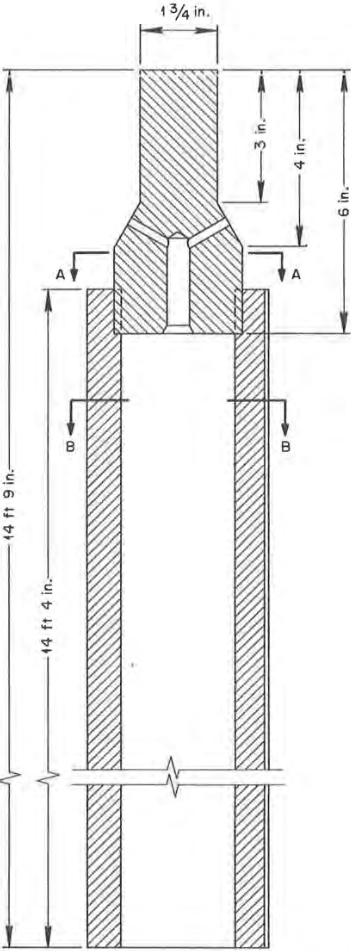
\includegraphics[width=0.25\linewidth]{figs/ch4/zone_iia_full_ref.png}
        \label{fig:msbr_iia_full_ref}
    }
    \subfloat[][]{
        
\includegraphics[width=0.17\linewidth]{figs/ch4/zone_iia_full_openmc.png}
        \label{fig:msbr_iia_full_model}
    }
    %\end{tabular}
    \caption[$xz$ cross sections of Zone II-A elements]{
        \subref{fig:msbr_iia_full_ref} Reference zone II-A element
        \subref{fig:msbr_iia_full_model} Model zone II-A element
    }
    \label{fig:msbr-iia-xz-full}
\end{figure}

\begin{figure}[htpb]
    \centering
    %\begin{tabular}{cc}
    \subfloat[][]{
        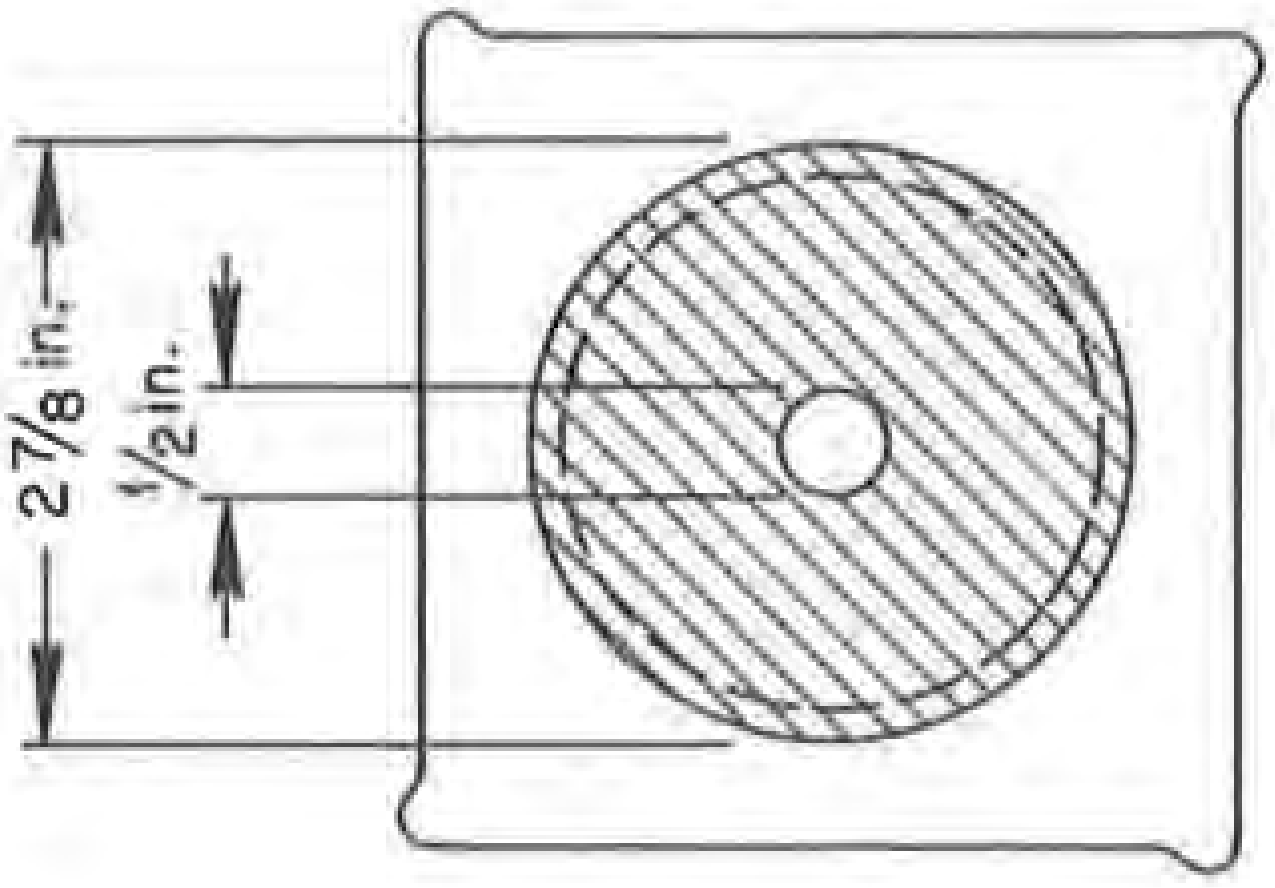
\includegraphics[width=0.3\linewidth]{figs/ch4/zone_iia_top_xy_ref.png}
        \label{fig:msbr_iia_top_ref}
    } 
    \subfloat[][]{
        
\includegraphics[width=0.2\linewidth]{figs/ch4/zone_iia_top_xy2_openmc.png}
        \label{fig:msbr_iia_top_model}
    }
    \\
    \subfloat[][]{
        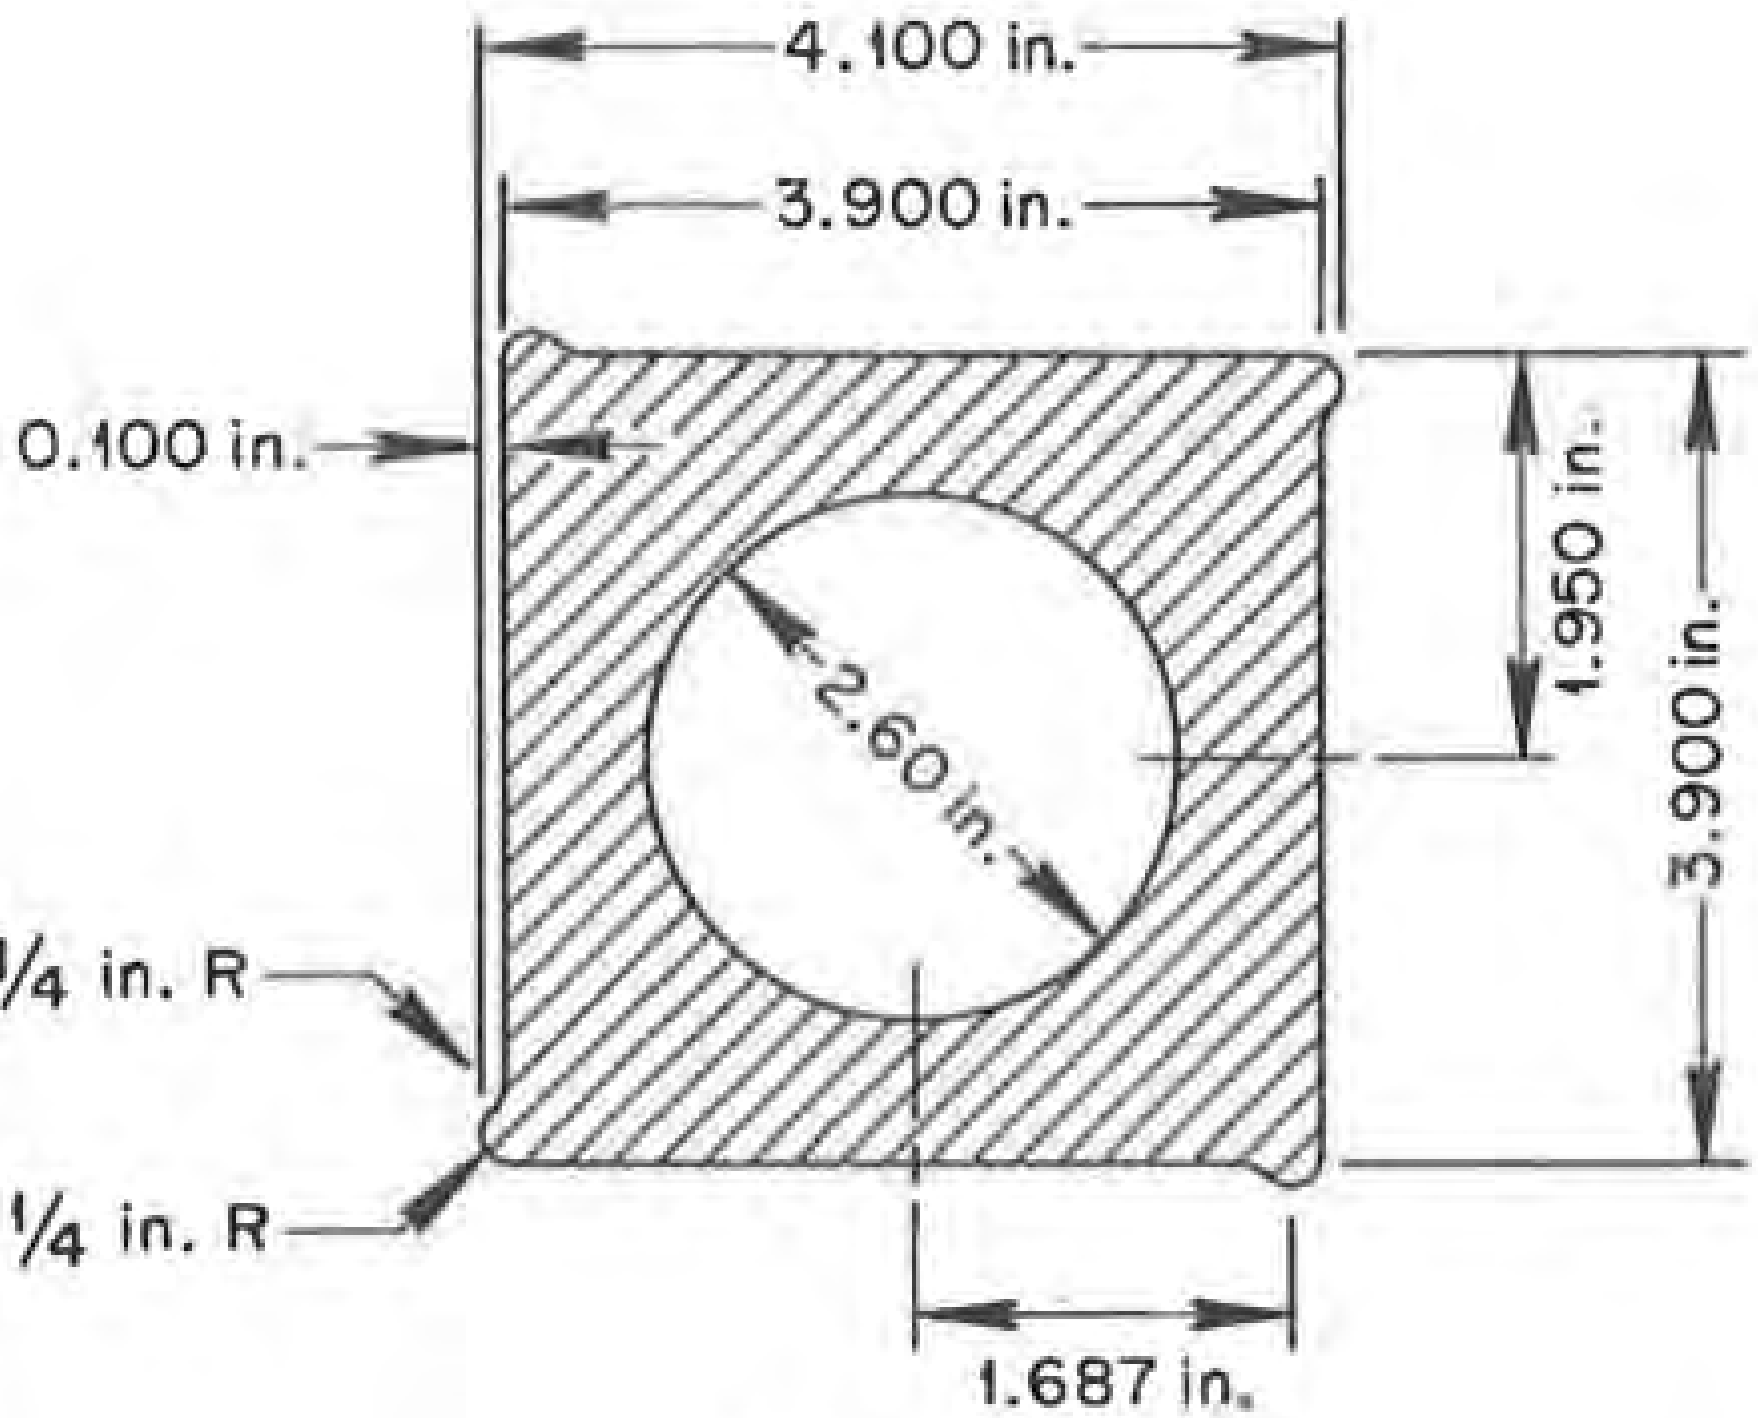
\includegraphics[width=0.35\linewidth]{figs/ch4/zone_iia_main_ref.png}
        \label{fig:msbr_iia_main_ref}
    } 
    \subfloat[][]{
        
\includegraphics[width=0.15\linewidth]{figs/ch4/zone_iia_main_openmc.png}
        \label{fig:msbr_iia_main_model}
    }
    %\end{tabular}
    \caption[$xy$ cross sections of Zone II-A elements]{
        \subref{fig:msbr_iia_top_ref} Reference zone II-A element; Section A.
        \subref{fig:msbr_iia_top_model} Model zone II-A element; Section A.
        \subref{fig:msbr_iia_main_ref} Reference zone II-A element; Section B.
        \subref{fig:msbr_iia_main_model} Model zone II-A element; Section B.
    }
    \label{fig:msbr-iia-xy}
\end{figure}

\subsection{Annulus}
A 2 in. wide annular space of 100-\% fuel salt separates zone II from the
graphite reflectors. The annulus serves as a clearance space when inserting or
removing the reactor core assembly, and provides some additional shielding to
extend the lifetime of the graphite reflectors \cite{robertson_conceptual_1971}. The annulus region is reproduced in full in the \Gls{csg} model. The annulus region is the dark teal section in between the brown and pink sections in Figure \ref{fig:msbr-cells}

\subsection{Reflectors}
\begin{figure}[htpb]
    \centering
    \subfloat[][]{
        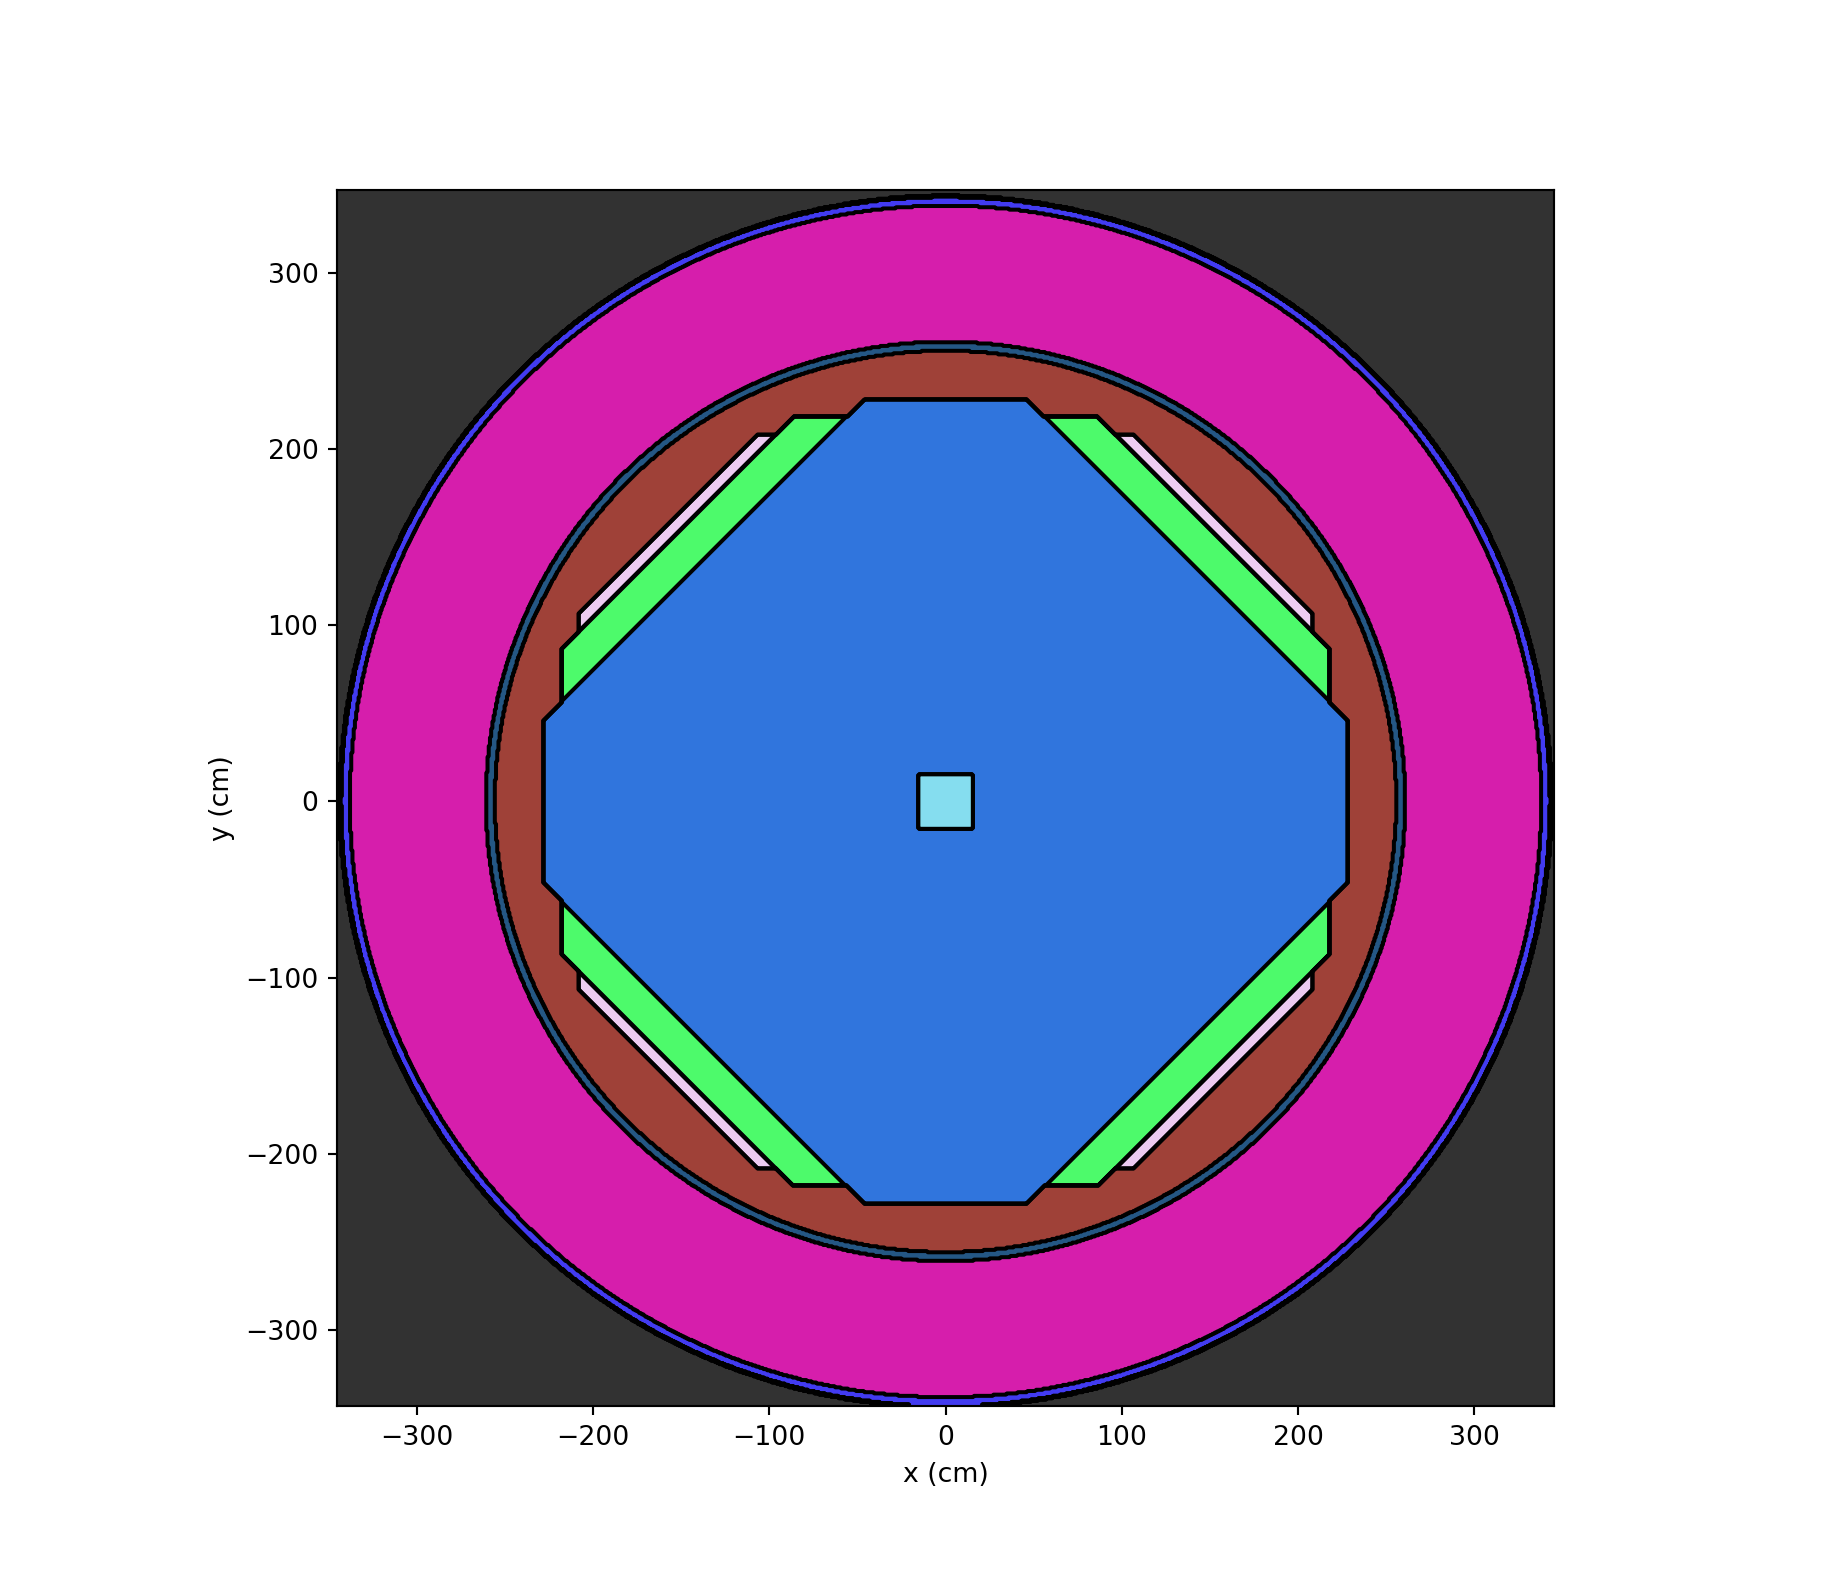
\includegraphics[width=0.5\linewidth]{figs/ch4/msbr_reduced_univs_xy.png}
        \label{fig:msbr-cell-xy}
    }
    \subfloat[][]{
        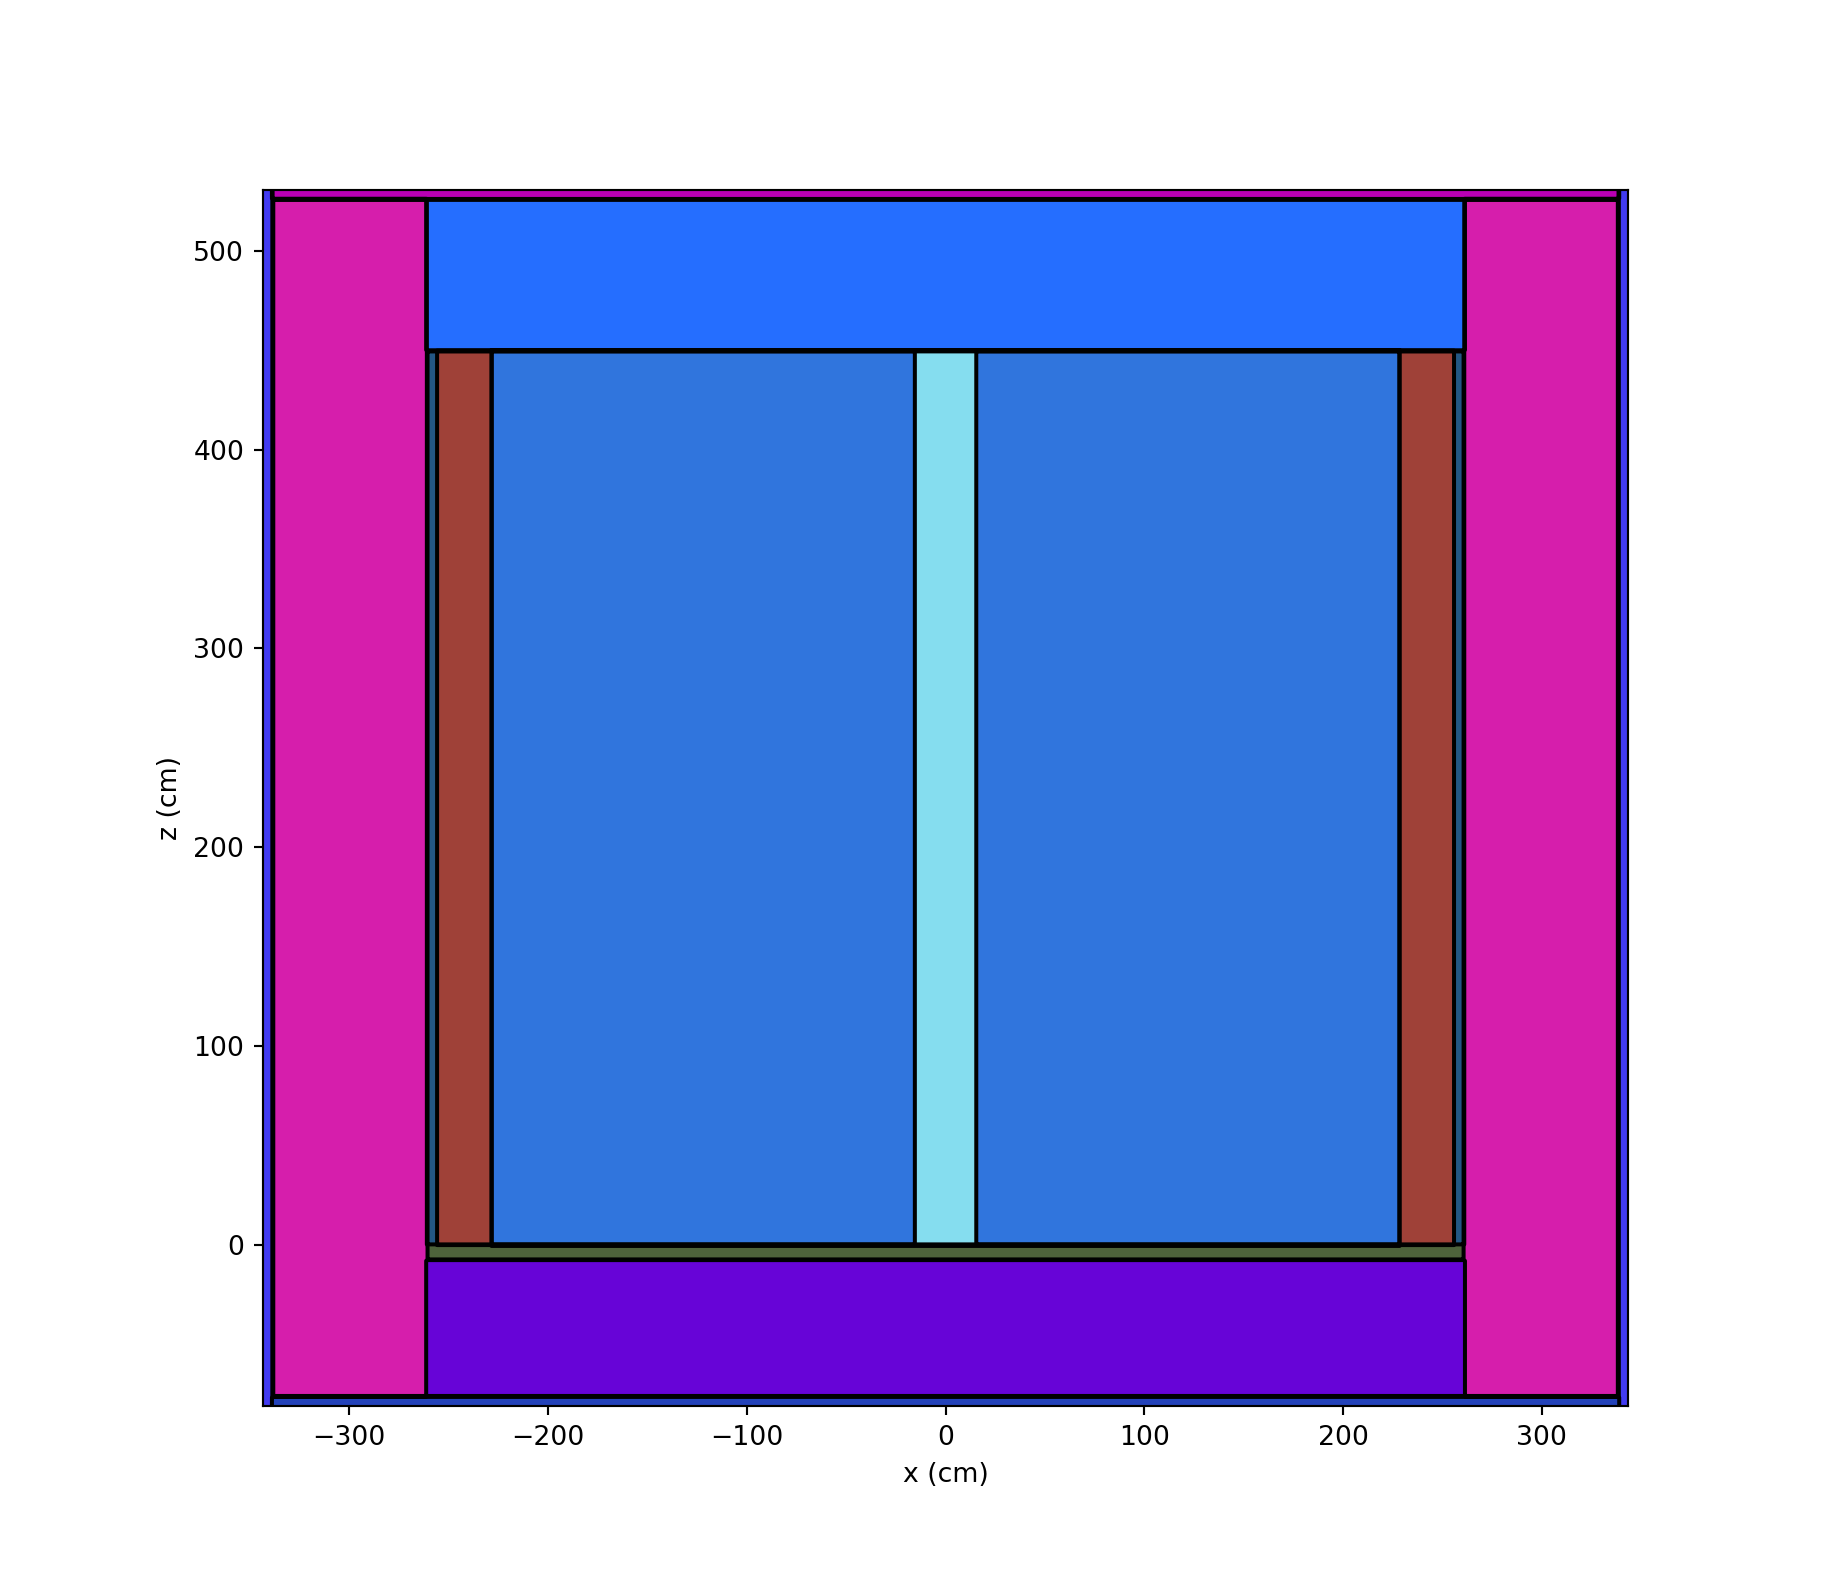
\includegraphics[width=0.5\linewidth]{figs/ch4/msbr_reduced_univs_xz.png}
        \label{fig:msbr-cell-xz}
    }
    \caption[MSBR CSG model cells]{MSBR CSG model cells.
        \subref{fig:msbr-cell-xy} $xy$ plane; 
        \subref{fig:msbr-cell-xz} $xz$ plane} 
    \label{fig:msbr-cells}
\end{figure}
The \Gls{msbr} has both axial and radial reflectors as seen in Figures
\ref{fig:msbr-overview} and \ref{fig:msbr-detail}. Both reflector regions are around 1\% fuel salt by volume. The radial
reflectors\footnote{I exclude the following details about the radial reflector
due to insufficient information in the report to reproduce them in a model:
modified Hastelloy N orifice plates, milled radial grooves at the bottom of each
reflector block, top layer blocks (see pages 15 and 16 in Robertson et al.
(1971))} consist of 29 in. (48.26 cm) thick wedge-shaped blocks that are 43 in. tall and 10 in. (25.4 cm) wide at the vessel wall and 9 in. wide at the inner end \cite{robertson_conceptual_1971}.
Four layers of these blocks comprise the entire radial reflector. Slots cut out
of the outer edge of the blocks facilitate modified Hastelloy N axial ribs to create a
0.25 in (0.635 cm) standoff space between the blocks and the vessel wall. Axial
flow from the reactor inlet through this space cools both the outer portion of
the reflector blocks and the vessel wall. Additionally, Robertson et al. (1971)
states that 1 in. graphite pins ``are inserted into the reflector pieces to hold
them apart'', but does not specify the position or number of these pins. These
pins create passages\footnote{these passages change dimension from 0.05 in. wide
while cold to 0.1 in. wide while hot \cite{robertson_conceptual_1971}} for
radial salt flow through the radial reflector region towards the annulus,
providing additional cooling. Modified Hastelloy N retaining rings placed in slots
between the block layers (see Figure \ref{fig:msbr-ref-xz}) ensure that the
position of the reflector blocks to the vessel wall stays relatively constant as
the materials expand under the heating of the fuel salt
\cite{robertson_conceptual_1971}.

The axial reflectors consist of wedge shaped graphite pieces (see Figure
\ref{fig:msbr-ref-xy}) that are 2 in. (5.08 cm) wide at the inner end and 16 in.
(40.64 cm) wide at the outer end \cite{robertson_conceptual_1971}. The dished
vessel heads cause the pieces to vary in thickness from 30 in. (76.2 cm) at the
center to 15 in. (38.1 cm) at the outer end (see Figure
\ref{fig:msbr-ref-xz}) \cite{robertson_conceptual_1971}. Robertson et al. (1971)
does not specify a length for the axial reflector pieces. 

The \Gls{csg} model approximates the complicated structure of the radial
reflector blocks as a hollow cylinder 601.98 cm tall and 77.216 cm thick, and
the axial reflector pieces as flat disks\footnote{the \Gls{csg} model does not
include the hole out of the top of the core for the control rods, and flattens
the dished shape as no dimensions are given to accurately reproduce the curvature
of the axial reflector pieces} 68.58 (bottom)/76.12 (top) cm thick and a radius
of 261.112 cm. The \Gls{csg} model also contains no fuel salt in the reflector
regions. Figure \ref{fig:msbr-cells} shows the radial reflector as a large pink
region, the top axial reflector as a light blue region, and the bottom axial
reflector as a purple region.

\section{Vessel}
\label{sec:msbr-vessel}
The \Gls{msbr} vessel is made of modified Hastelloy N, and has a wall thickness
of 2 in. unless otherwise specified \cite{robertson_conceptual_1971}. The vessel
is broken into the following sections:
\begin{enumerate}
    \item The main wall: a 13 ft. tall cylindrical section with an outer
    diameter of 22.5 ft. This section is the main contact surface for the axial
    reflectors.
    \item The transition section: A 4 ft. tall conical section. The conical base
    has a diameter of ~22.5 ft. and the conical ``roof'' has a diameter of ~18
    ft. This section connects the main wall to the support section and contains
    the salt outlet nozzles.
    \item The nested support sections: two ~13.5 ft tall cylindrical sections
    that nest. Both sections have a 2 in. wall thickness. The outer cylinder has
    an inner diameter of 18 ft, and the inner cylinder has an outer diameter of
    slightly less than 18ft to allow for clearance to fit the two pieces
    together. The assembly is flanged at the top to close the vessel. The
    flanged support section is also the main point of contact with the
    reinforced concrete roof structure from which the reactor hangs.
    \item The dished head sections: both heads have a 3 in. wall thickness. The
    lower head has a 22.5 ft diameter and the upper head an 18 ft. diameter. No
    radius of curvature is given for the dished heads, but it may be possible to
    determine the shape using the given dimensions and other dimensions of the
    vessel.
\end{enumerate}

The CSG model representation of the vessel has a 2 in. (5.08
\unit{\centi\metre}) thickness, and hugs the radial region in the CSG model,
giving an outer diameter of 22.53 ft. (686.816 \unit{\centi\metre}) and a
height of 20.08 ft (612.14 \unit{\centi\metre}). The CSG model does not include
the nested support sections as they are of little neutronic importance. Figure
\ref{fig:msbr-cells} shows the radial vessel as a thin blue region at the outer
edge of the radial reflector region, and the axial vessel as a thin pink region
at the outer edge of the axial reflector regions.

\section{An aside on the salt volume}
\label{sec:salt-volume}
The original salt volume in the \Gls{csg} \Gls{msbr} model was set to
$4.871\cdot 10^7$ \unit{\centi\metre\cubed}. This is roughly double the salt
volume in the core in the reference specification (see Table
\ref{tab:salt-volumes}). I performed stochastic volume calculations on both the
\SerpentTWO and \OpenMC versions of the \Gls{csg} model, and found they both
calculated volumes around $2.6\cdot 10^7$ \unit{\centi\metre\cubed}. Averaging
the two volumes gives a roughly 8\% error in the salt volume in the core compared
to the reference specification (see Table \ref{tab:stoch-vol}).

\begin{table}[htpb]
    \centering
    \caption[MSBR fuel stochastic volume calculations]{MSBR fuel stochastic volume calculations, using $1\cdot 10^9$ particles.}
    \label{tab:stoch-vol}
    \begin{tabular}{|c|c|c|c|}
        \hline
        Quantity & \SerpentTWO & \OpenMC & Average\\
        \hline
        Volume [\unit{\centi\metre\cubed}] & $2.60961 \cdot 10^7$ & $2.6085 \cdot 10^7$ & $2.6091 \cdot 10^7$ \\
        \hline
        Statistical error & 0.00010 & 0.00010 & 0.00007 \\
        \hline
    \end{tabular}
\end{table}

For depletion without reprocessing this new volume would be correct to
use for our geometry. When we assume that we are performing online reprocessing,
we must account for all of the salt in the core {\it and} the salt in the
primary loop as this salt is routed through the processing components. Table S.1
in \cite{robertson_conceptual_1971} gives us the total volume of salt in the
primary system as  1720 ft$^{3}$ ($4.8705\cdot 10^7$ \unit{\centi\metre\cubed}).
This value is valid assuming that we have reproduced the core geometry exactly
as specified, however in the \Gls{msbr} reference design, the total volume of
salt in the reactor vessel is 1074 ft$^{3}$ ($3.0412 \cdot 10^{7}$
\unit{\centi\metre\cubed}) \cite{robertson_conceptual_1971}, which is 
approximately 13\% greater than the geometrical volume of the salt. This
discrepancy is due to the absence of the core inlets, outlets, and the narrow
salt passages in the reflector region. These features are important for thermal
hydraulic accuracy, however they are most likely not particularly neutronically
important. Additionally, we want to stay as consistent as possible with
Rykhlevskii's previous works \cite{rykhlevskii_fuel_2020}
\cite{rykhlevskii_modeling_2019}, so we will use the existing value for the salt
volume of $4.871\cdot 10^7$. \unit{\centi\metre\cubed}. This choice carries the
implicit assumption that we are applying the neutronic conditions in the core to
$4.871\cdot 10^{7}$ \unit{\centi\metre\cubed} of salt during the entire
depletion step, which does not account for the actual salt processing rate and
fuel salt mass flowrate\footnote{According to Table S.1 in Robertson et al.
(1971), the cycle time for the salt inventory in the primary system is 10 days
\cite{robertson_conceptual_1971}}. To do so would require development of
SaltProc that is outside the scope of this thesis.

%% Table 3.2 and 3.3 in robertson
\begin{table}[htpb]
    \centering
    \caption[Volume of salt in reference MSBR core regions]{Volume of salt in
reference MSBR core regions. Reproduced from Table 3.2 in
\cite{robertson_conceptual_1971}}
    \label{tab:salt-volumes}
    \begin{tabular}{|c|c|cc|}
        \hline
        Zone & Percent salt & Salt volume [ft$^3$] & Salt volume [\unit{\metre\cubed}] \\
        \hline
        Zone I & 13.2 & 288 & 8.155252 \\
        \hline
        Zone II & 37 & 376.5 & 10.661293 \\
        \hline
        Upper plenum & 85 & 36.2 & 1.02507 \\ 
        \hline
        Lower plenum & 100 & 35.4 & 1.002416 \\ 
        \hline
        Annulus & 100 &  132 & 3.737824\\
        \hline
        Core total & - & 868.1 & 24.581855 \\ 
        \hline
    \end{tabular}
\end{table}

\section{Reprocessing system}
\label{sec:msbr-reprocessing-system}
The MSBR reference design included the specification of a fuel-salt processing
system\footnote{For this thesis, processing refers to both gas removal and
chemical processing}. The purpose of this reprocessing system is to improve
neutronic performance by removing neutron poisons and other contaminants from
recirculating through the core. The reprocessing system is split into two parts:
gas removal and chemical extraction. The gas removal system takes advantage
of entrainment of insoluble species in helium bubbles to remove noble gas
fission products from the fuel salt. The reprocessing system is based on
reductive extraction\footnote{Reductive extraction takes advantage of the higher
electronegativity of a particular element to drive reduction reactions that
remove target elements from covalently bonded molecules}. I will provide a brief
description of the entire reprocessing system, but justifying in and evaluating
its efficacy are beyond the scope of this thesis\footnote{I encourage interested
readers to look at chapters 7 and 8 in \cite{robertson_conceptual_1971}, the
entirety of \cite{carter_design_1972} and \cite{lindauer_design_1969}, as well
as the molten salt reactor program semiannual progress reports, all of which you
can find at \url{energyfromthorium.com/pdf}}.

\begin{figure}[htpb]
    \centering
    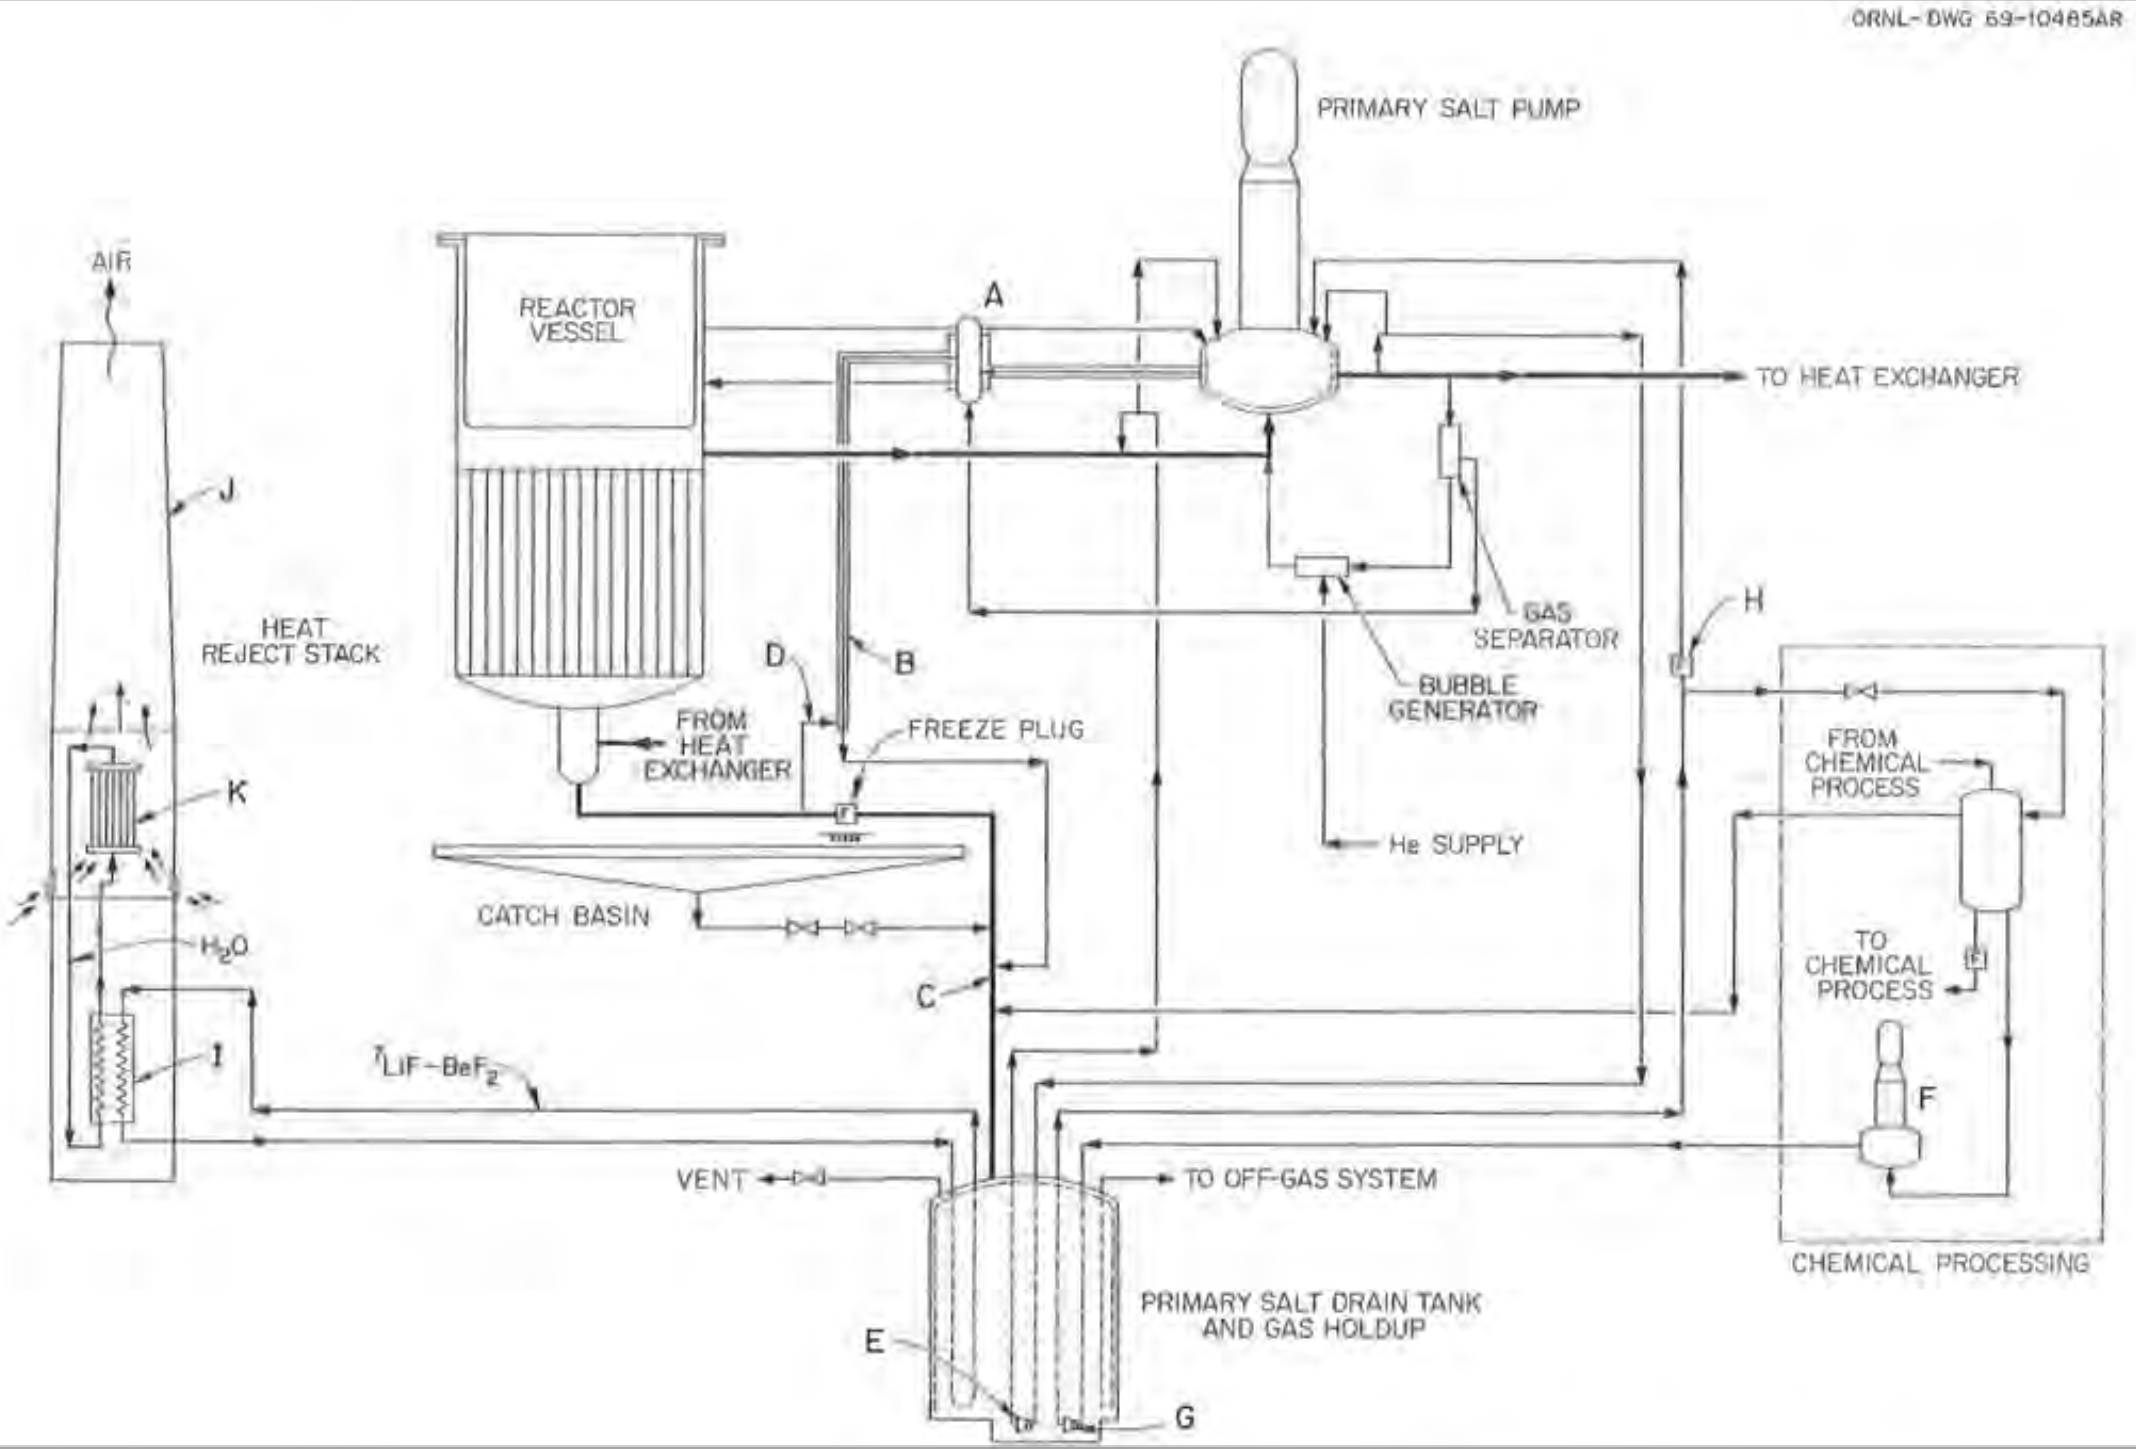
\includegraphics[width=0.8\textwidth]{figs/ch4/msbr_primary_system.png}
    \caption{Simplified flow diagram of primary drain tank and heat removal
    system. Reproduced from Figure 2.3 in \cite{robertson_conceptual_1971}. (A)
    Combiner tank for separated gases and overflow salt, (B) Off-gas line with
    cooling jacket, (C) Fuel-salt drain line, (D) Drain line continuous bleed
    flow, (E) Jet pumps from returning overflow fuel salt to primary system, (F)
    Ancillary fuel-salt transfer pump, (G) Jet pump for filling primary system
    and sending salt to chemical processing, (H) Freeze-plug type valve }
    \label{fig:msbr_primary_system}
\end{figure}

\subsection{Gas removal system}
The gas removal system removes short-lived neutron poisons gases (tritium,
xenon, and krypton) from returning to the core region. There are three
components to this system: the bubble generator, the gas separator, and the
off-gas system. The gas separator is where the physical separation of the
neutron poisons from the fuel salt occurs.

The bubble generator creates bubbles from helium gas injected into the fuel
salt\footnote{the phenomena of pockets of gas trapped in pockets, along with any
other material they may pick up, and transported in fluid flow is called {\it
entrainment}. The \Gls{msbr} includes a salt entrainment separator downstream
from the gas separator that removes entrained salt and metal contaminants from
the helium bubbles before the gas is processed. See Section 5.3 in
\cite{rosenthal_molten-salt_1968}}. These helium bubbles will pick up the
fission product gases and carry them on the interface between the helium and the
salt. This process is called {\it sparging}. Around 10\% of the total salt flow
is routed from the primary pumps into this system. Figure
\ref{fig:gas_removal_system} provides an overview.

\begin{figure}[htpb]
    \centering
    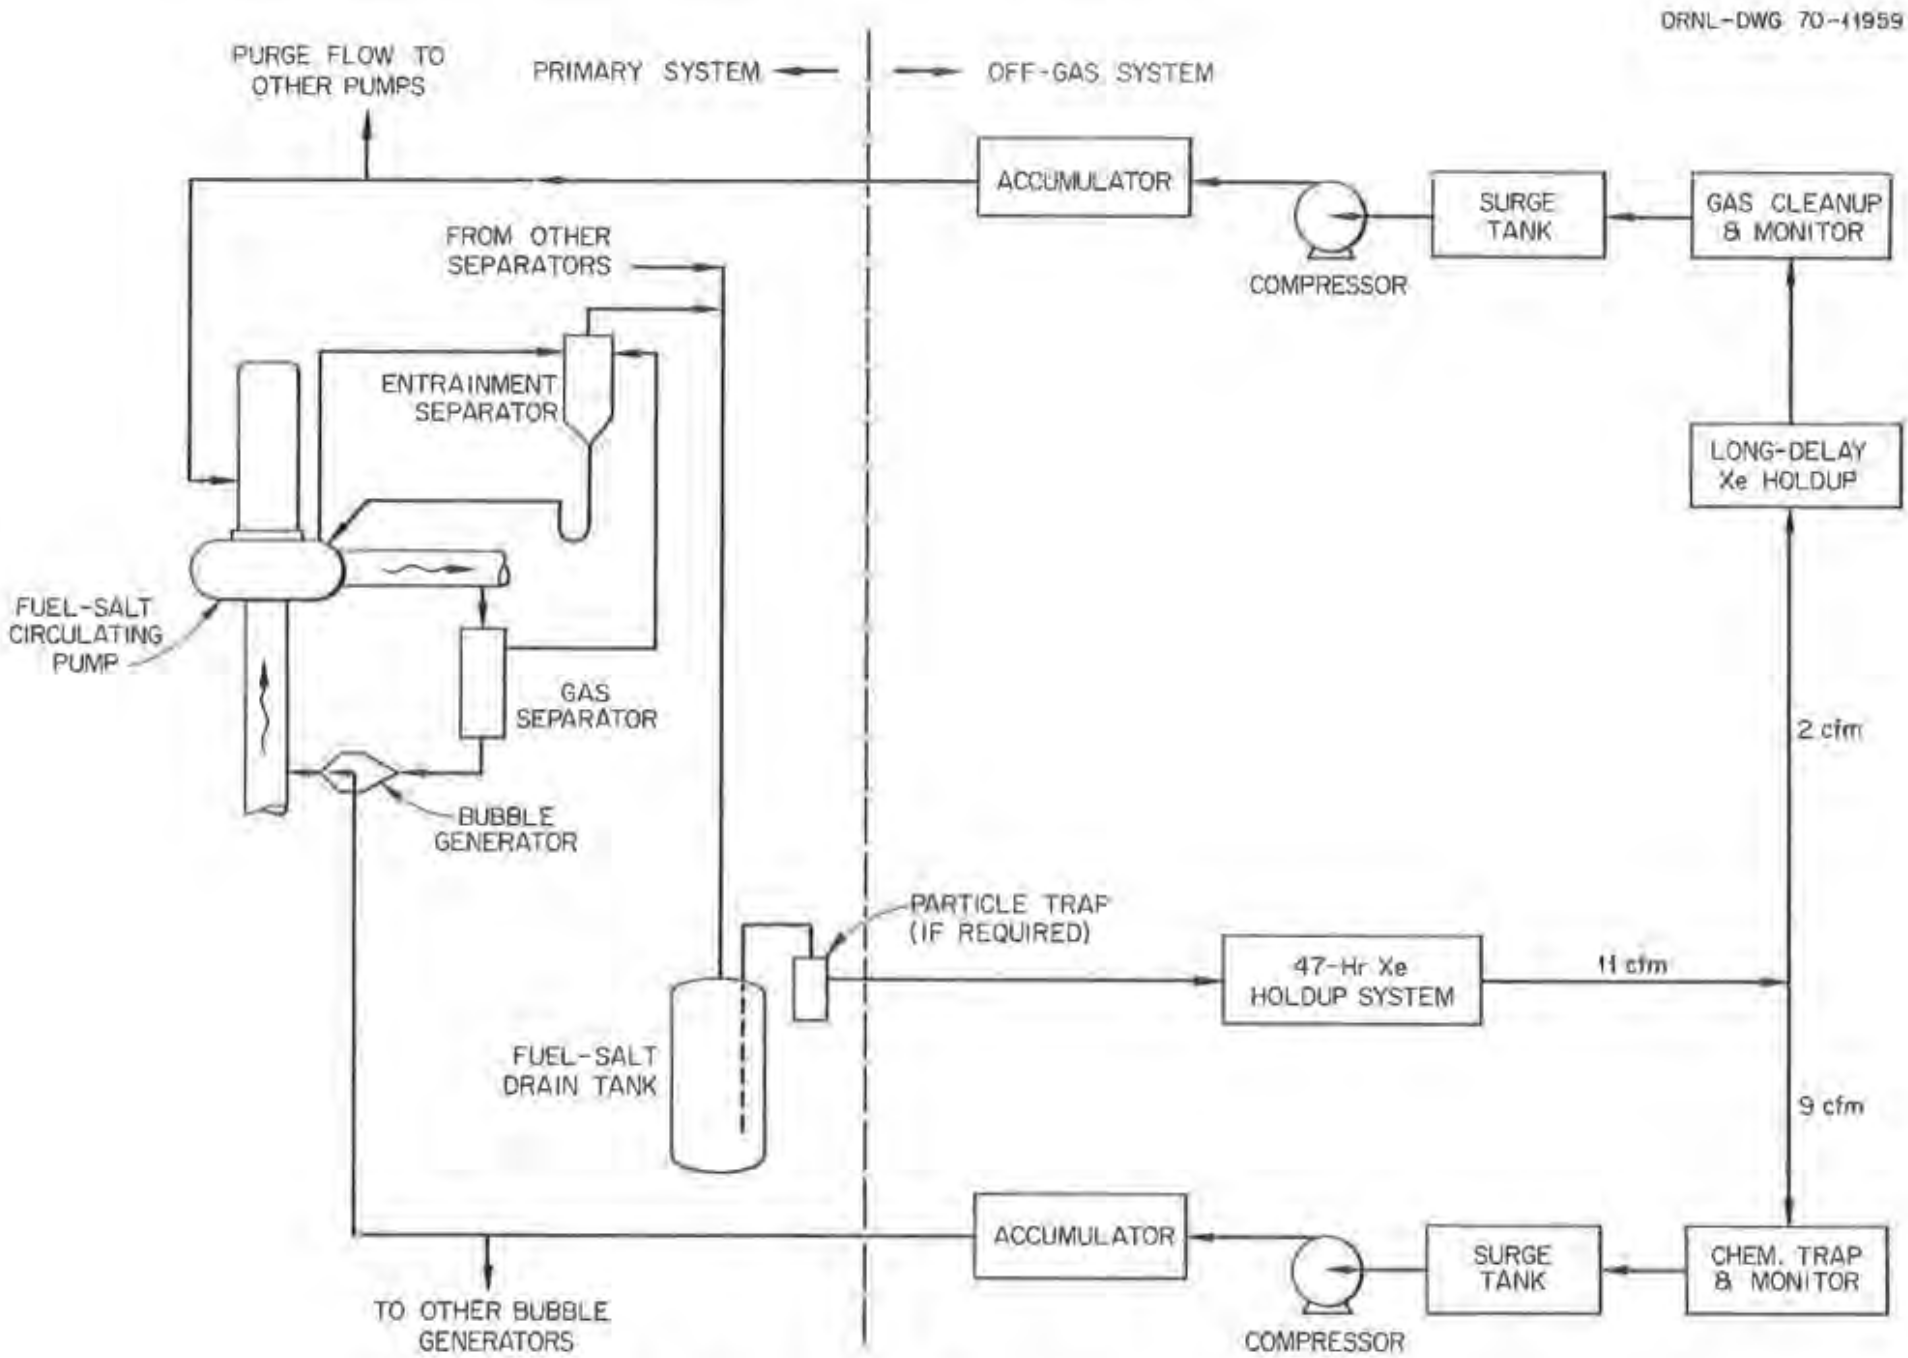
\includegraphics[width=0.8\textwidth]{figs/ch4/gas_removal_system.png}
    \caption{Overview of \Gls{msbr} gas removal system. Reproduced from Figure 7.1 in \cite{robertson_conceptual_1971}}
    \label{fig:gas_removal_system}
\end{figure}

The main purpose of the off-gas system is to separate the helium from the
fission product gasses for reuse in sparging. We only care about the
corresponding extraction efficiency of the fission product gases, so we do
not include the off-gas system in our model. Interested readers should reference
Chapter 7 in Robertson et al. (1971) \cite{robertson_conceptual_1971}.

\subsection{Fuel salt drain tank}
In addition to providing a emergency salt storage system in the case of
electrical system failure, the fuel salt drain tank plays an important role in
the fuel-salt reprocessing system \cite{robertson_conceptual_1971}. The drain tank catches around 150 gpm (approximately 0.9\% of the total salt flow) of
overflow from the primary salt circulation pumps, providing it with a small
amount of salt during operation \cite{robertson_conceptual_1971}. A 0.88 gpm
stream of salt from the drain tank flows through the chemical processing system
and back to the drain tank. Jet pumps at the bottom of the drain tank send salt
back to the primary loop. Figure \ref{fig:msbr_primary_system} shows this
arrangement.

\subsection{Chemical processing system}
The chemical processing system has two purposes:
\begin{enumerate}
    \item To isolate \ce{^{233}Pa} from the high neutron flux zone to allow it to decay into \ce{^{233}U}
    \item To remove impurities (rare earth metals) and fission products from the fuel salt
\end{enumerate}

\begin{figure}[htpb]
    \centering
    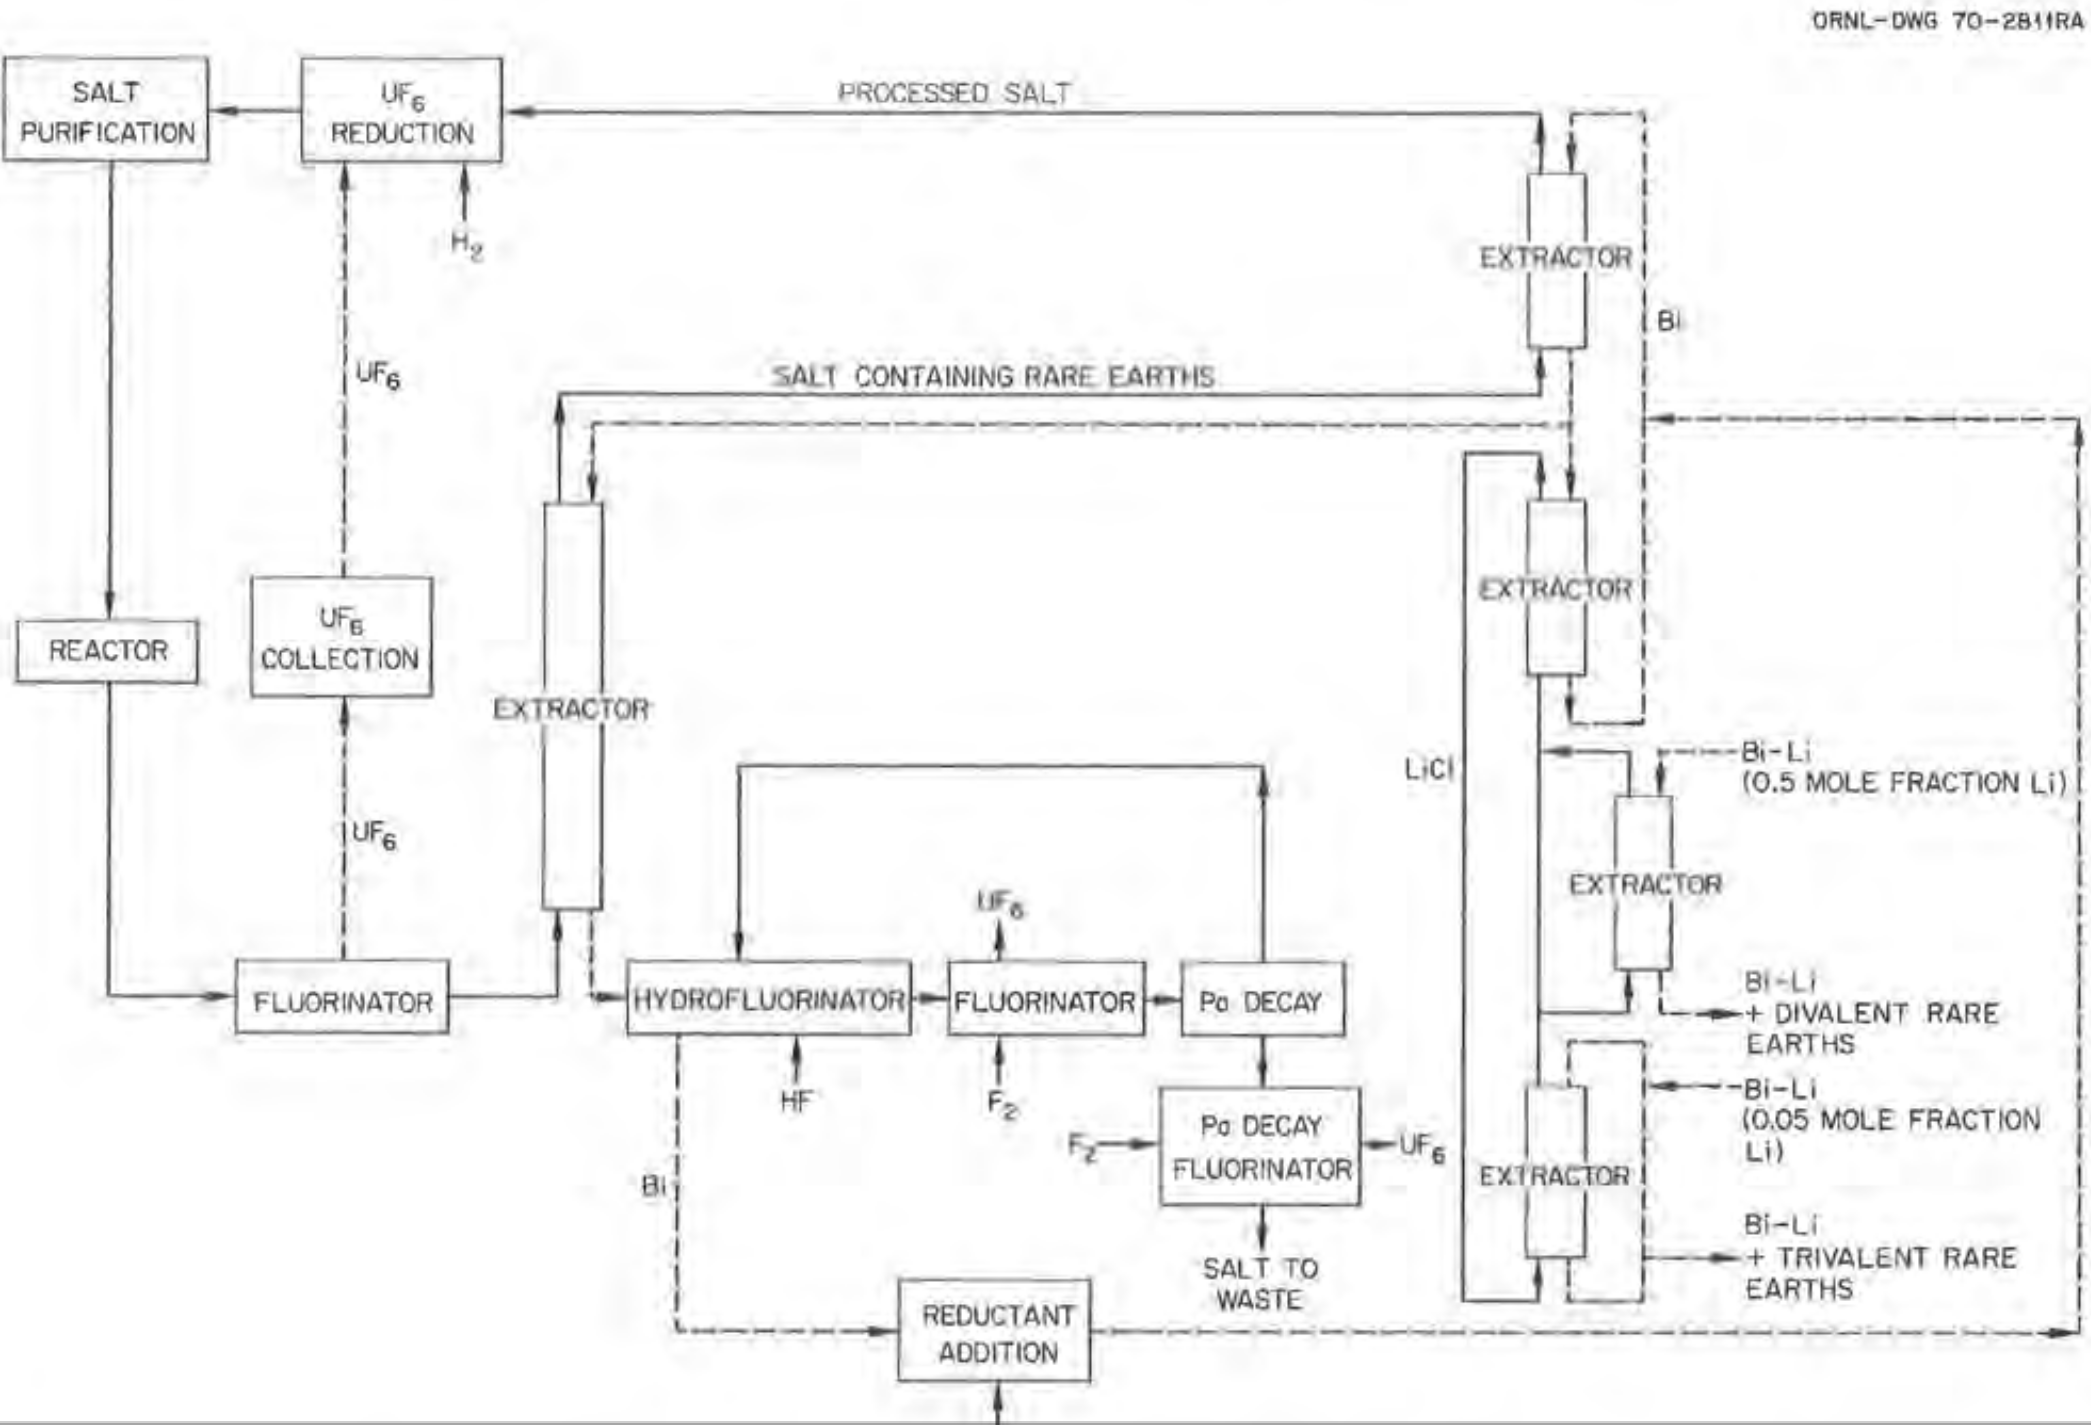
\includegraphics[width=0.8\textwidth]{figs/ch4/chemical_processing_system.png}
    \caption{Chemical processing system overview. Reproduced from Figure 2.4 in \cite{robertson_conceptual_1971}}
    \label{fig:}
\end{figure}

\paragraph{Protactinium isolation loop}
In order to remove the protactinium from the fuel salt, all uranium must first be removed. The protactinium isolation loop consists of several components: 
\begin{enumerate}
    \item A fluorinator to remove 95\% of the uranium in the fuel salt.
    \item An extraction column where the stream leaving the fluorinator is combined with a stream of bismuth and thorium that removes protactinium and additional uranium from the fuel salt. The salt stream leaving the extractor is routed to the rare metal removal system. This salt stream has nearly no protactinium or uranium in it.
    \item A hydrofluorinator where the stream leaving the extraction column removes the thorium, lithium, and uranium from the bismuth. The bismuth is sent to a reductant adder where lithium is added to the bismuth stream, and then is rerouted back to the extraction column.
    \item A second fluorinator that removes 95\% of the remaining uranium from the stream leaving the extraction column.
    \item A protactinium decay tank into which the stream leaving the second fluorinator flows. This stream is circulating as it feeds back to the hydrofluorinator for additional uranium removal. Uranium produced by protactinium decay is removed by this circulating stream.
\end{enumerate}

The uranium extracted via fluorination is returned to 
Figure \ref{fig:pa-removal} shows a block diagram of this loop. 

\begin{figure}[htpb]
    \centering
    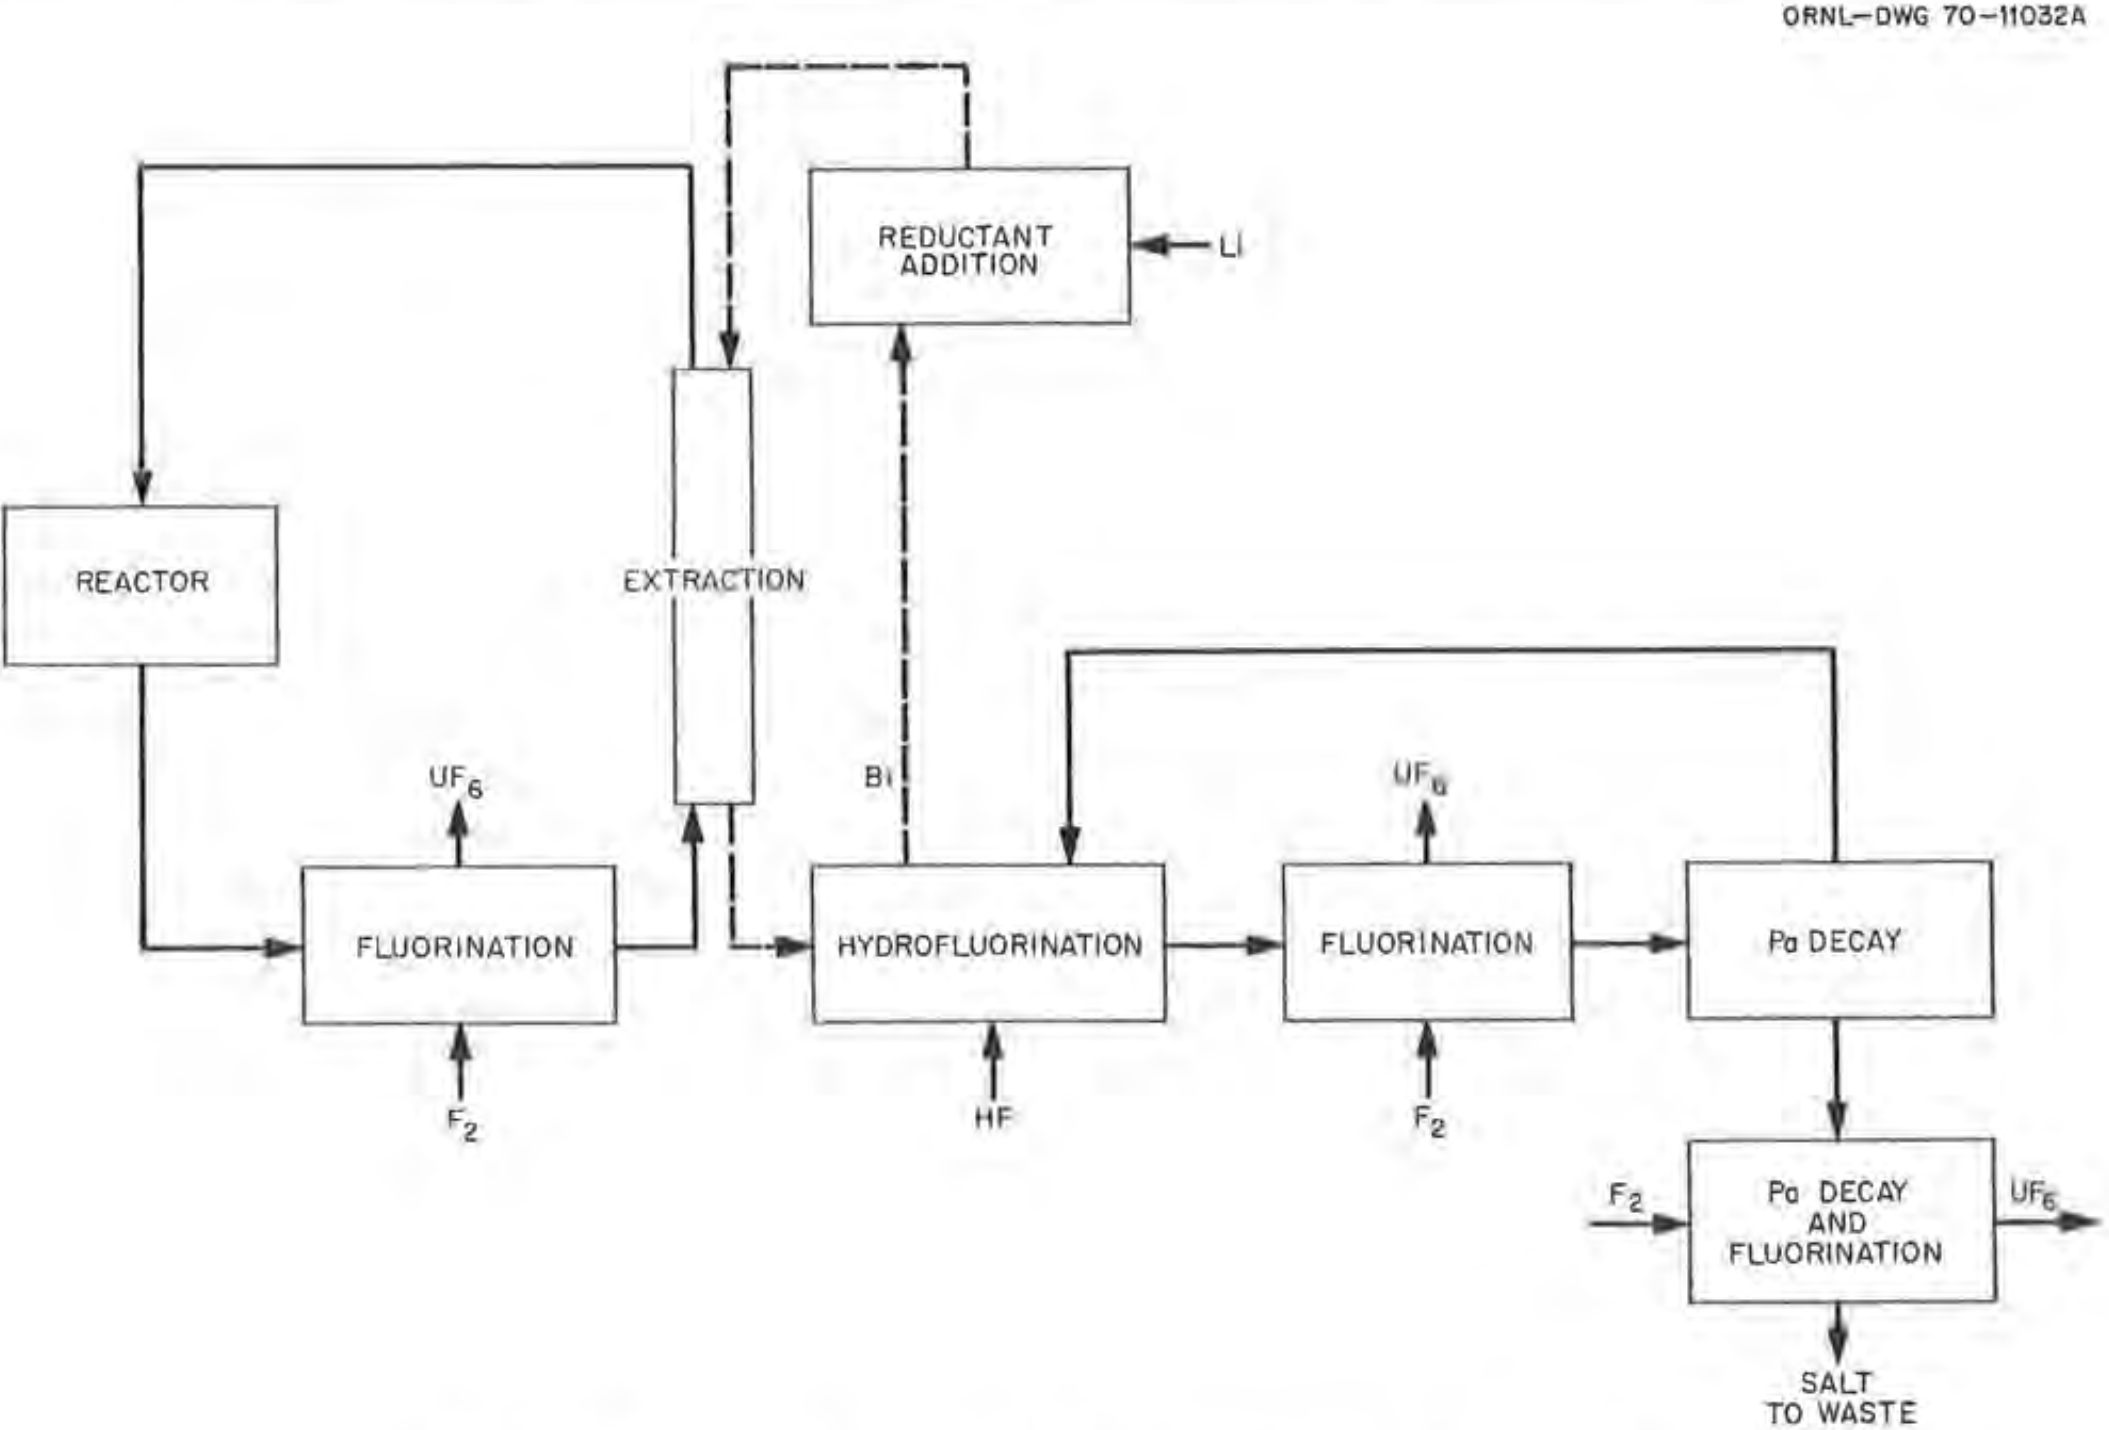
\includegraphics[width=0.8\textwidth]{figs/ch4/pa_removal_loop.png}
    \caption{\ce{^{233}Pa} removal loop. Reproduced from Figure 8.1 in \cite{robertson_conceptual_1971}}
    \label{fig:pa-removal}
\end{figure}

\paragraph{Rare-earth removal system}
The rare-earth removal system utilized the same metal transfer process used to
isolate protactinium from the fuel salt \cite{robertson_conceptual_1971}. This
system begins at the output of the extractor column for protactinium isolation.
It is a multistage extraction system:
\begin{enumerate}
    \item In the first extractor, the salt stream from the protactinium loop
    extractor column is contacted with a bismuth stream containing 0.2 mol-\%
    lithium and 0.25 mol-\% thorium. The bismuth stream picks up a fraction of
    the rare earths and routes to the second extractor.
    \item In the second extractor, the bismuth stream containing rare earths is
    contacted with a \ce{LiCl} stream.  The \ce{LiCl} stream picks up a fraction
    of the rare earths (with trace amounts of thorium), and is routed to the
    fourth extractor. The bismuth stream is returned to the first extractor.
    \item In the fourth extractor, the \ce{LiCl} stream is contacted with a
    circulating bismuth stream containing 5 mol-\% lithium. This bismuth stream
    removes trivalent rare earths from the \ce{LiCl} stream. The \ce{LiCl}
    stream is returned to the second extractor, however 2\% of this \ce{LiCl}
    stream is routed to the third extractor.
    \item In the third extractor, the \ce{LiCl} stream is contacted with a
    circulating bismuth stream containing 50 mol-\% lithium. This bismuth stream
    removes divalent and alkaline rare earths from the \ce{LiCl} stream. The
    \ce{LiCl} stream is rerouted back to the second extractor.
\end{enumerate}

Figure \ref{fig:metal-removal} shows a block diagram of this loop. 

\begin{figure}[htpb]
    \centering
    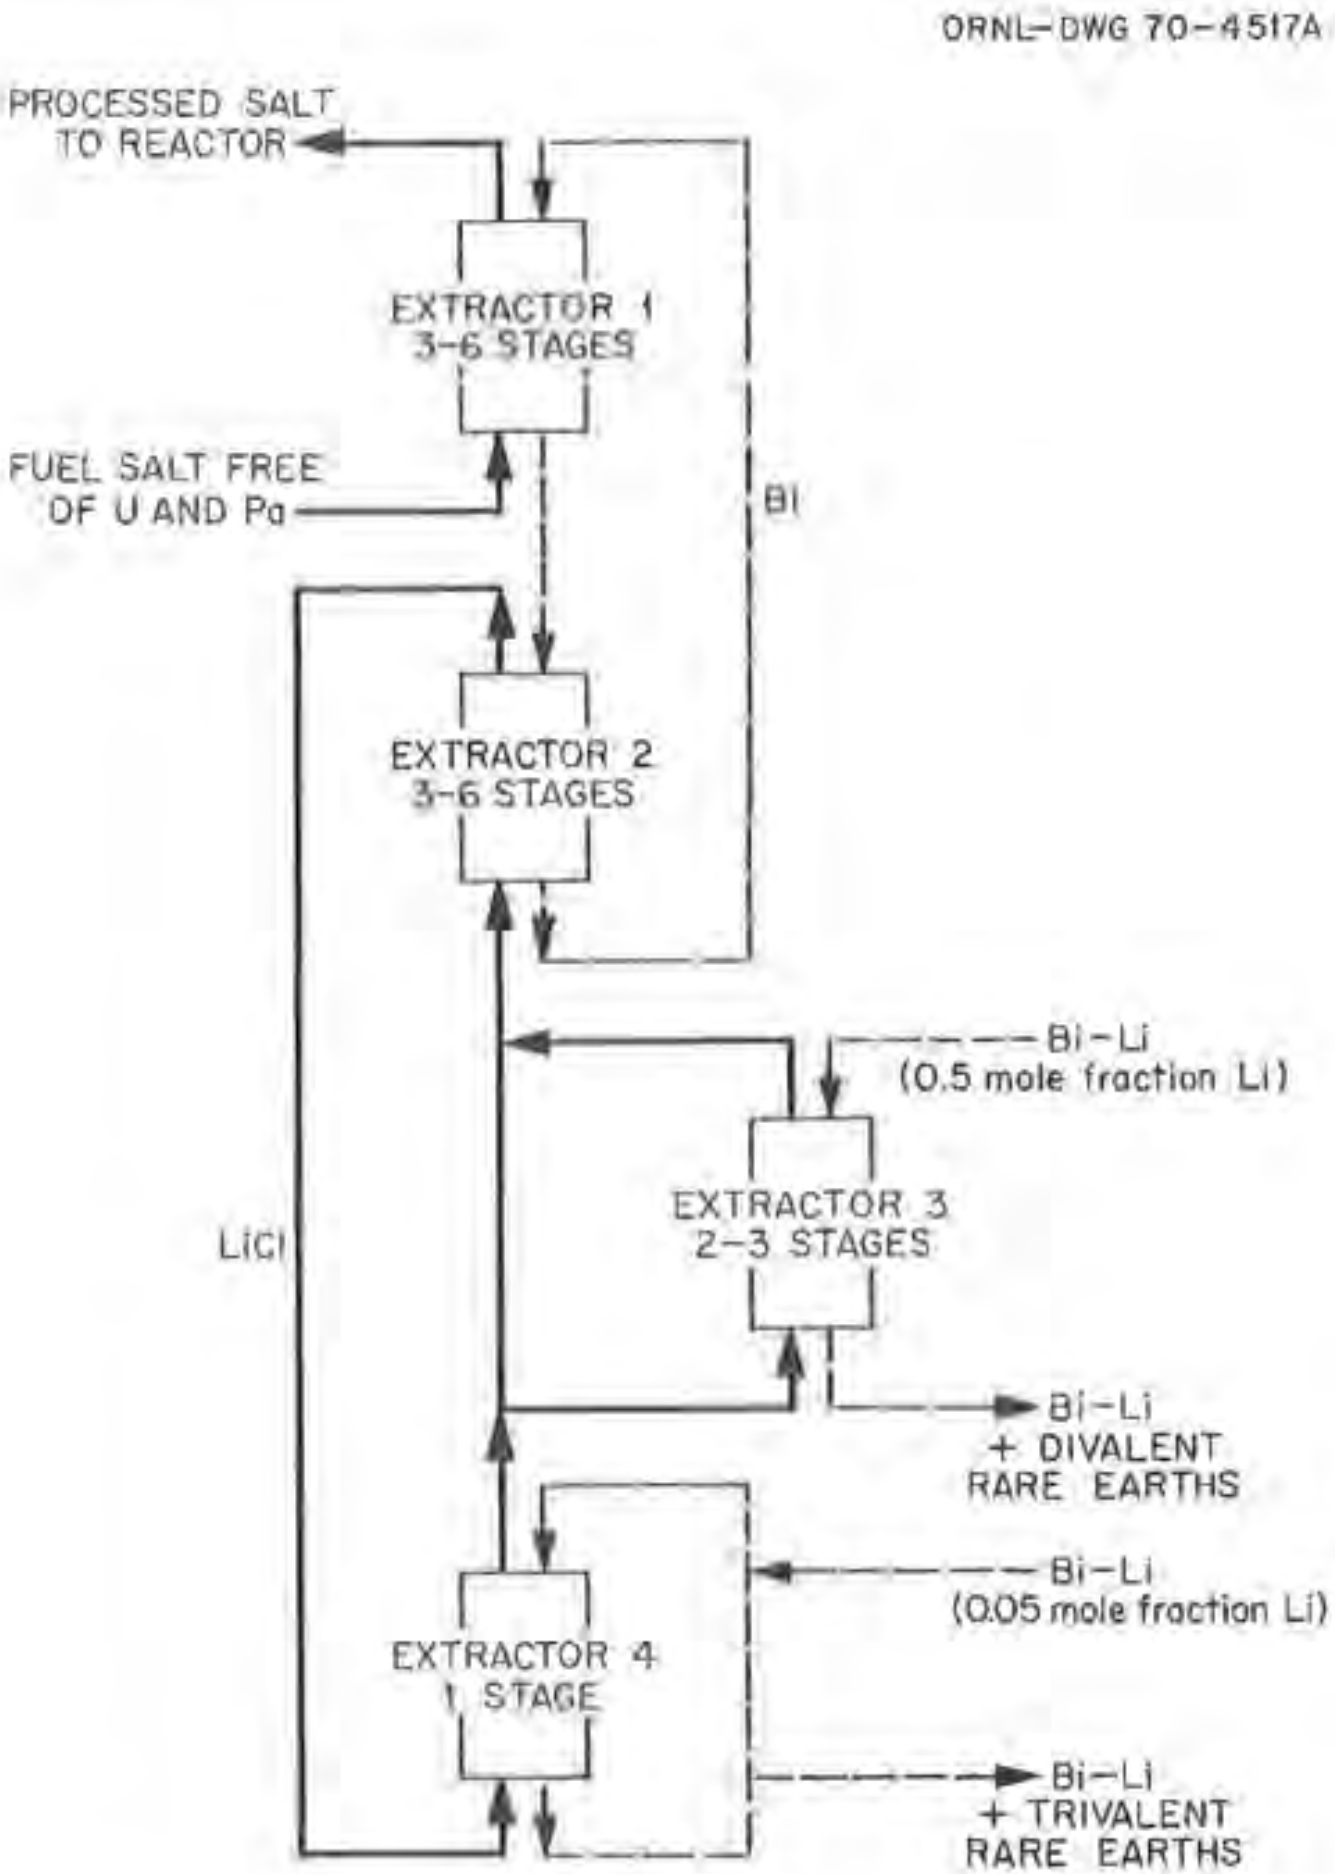
\includegraphics[width=0.3\textwidth]{figs/ch4/metal_removal_loop.png}
    \caption{Metal removal loop. Reproduced from Figure 8.2 in \cite{robertson_conceptual_1971}}
    \label{fig:metal-removal}
\end{figure}

\paragraph{Nickel-mesh filter}
Insoluble impurities in the processed salt needs to be removed at two locations:
before the salt stream is sent to reductive extraction system
\cite{lindauer_design_1969}, and before the processed salt stream coming
from the reductive extraction system returns to the
reactor \cite{robertson_conceptual_1971}. The first filter removes insoluble
impurities from transmutation and corrosion in the core, heat exchanger, and
other systems. The second filter removes  bismuth entrained or dissolved in the
fuel salt as a side effect from processing, and any additional insoluble
impurities such as \ce{FeF_2} and \ce{NiF_2}. The filter itself consists of a
nickel mesh \cite{robertson_conceptual_1971}.


\subsection{Reprocessing system model}
As described in Section \ref{sub:feeds-separations}, SaltProc relies on extraction efficiencies to model chemical removal of target elements from the fuel salt.  Unfortunately, Robertson et al. (1971) 
\cite{robertson_conceptual_1971} provide no such values, and a literature review
to find such values is outside the scope of this thesis. What Robertson does
give us are the cycle times for elements in the fuel salt.

\begin{table}[htpb] 
    \centering 
    \caption{Reprocessing system cycle times. A combination of tables 3.7B in \cite{robertson_conceptual_1971}, Table 3 in \cite{carter_design_1972}, and Table 25.1 in \cite{rosenthal_molten-salt_1970}}
    \label{tab:msbr-cycle-times}
    \begin{tabularx}{500pt}{|X|X|X|X|X|} 
        \hline
        Processing group & Target component(s) & Cycle time for processing & Primary mechanism of removal from salt & Secondary mechanism of removal from salt\\
        \hline
        Protactinium & \ce{^{233}Pa} & 3 days & Reductive extraction with \ce{Bi-Li} in \ce{Pa} extraction column followed by isolation in \ce{Pa} decay salt & None \\
        \hline
        Rare earths & Trivalent: \ce{Y}, \ce{La}, \ce{Ce}, \ce{Pr}, \ce{Nd}, \ce{Pm}, \ce{Gd}, Divalent: \ce{Sm}, \ce{Eu} & 50 days (500 for \ce{Eu}) & Reductive extraction with \ce{Bi-Li} in \ce{Pa} extraction column followed by isolation in \ce{Pa} decay salt & Reduction to metallic particulates by \ce{H_2} in reduction column followed by filtration\\
        \hline 
        Noble metals & \ce{Se}, \ce{Nb}, \ce{Mo}, \ce{Tc}, \ce{Ru}, \ce{Rh}, \ce{Pd}, \ce{Ag}, \ce{Sb}, \ce{Te} & 20 sec & Plating out on surfaces in reactor vessel and heat exchangers & \ce{Nb}, \ce{Mo}, \ce{Tc}, \ce{Ru}, \ce{Rh},\ce{Sb}, and \ce{Te} have volatile fluorides and are removed in fluorinators; \ce{Pd}, \ce{Ag } reduced by \ce{Bi-Li} alloy in reductive extraction.\\
        \hline
        Seminoble metals & \ce{Zr}, \ce{Cd}, \ce{In}, \ce{Sn} & 200 days & Plating out on surfaces in ractor vessel and heat exchangers & Reductive extraction with \ce{Bi-Li} in \ce{Pa} extraction column followed by isolation in \ce{Pa} decay salt \\
        \hline
        Gases & \ce{Kr}, \ce{Xe} & 20 sec & Sparged from salt with \ce{He} gas in primary loop & Purged in fluorniators due to sparging action of \ce{F_2} and \ce{H_2}\\
        \hline
        Halogens & \ce{Br}, \ce{I} & 60 days & Volatilization in primary fluorinator & None \\
        \hline
        Carrier salt & \ce{Th}, \ce{Li}, \ce{Be}, \ce{F} & 3435 days & Fuel salt discard to remove excess \ce{Li} added in reductive extraction process. & None \\
        \hline
        Alkaline earths; alkali metals & \ce{Sr}, \ce{Ba}; \ce{Rb}, \ce{Cs} & 3435 days & Fuel salt discard & None \\
        \hline
    \end{tabularx}
\end{table}

Rykhlevskii previously used 100\% extraction efficiency with 3-day depletion
steps \cite{rykhlevskii_modeling_2019} using SaltProc v0.1.0. As mentioned in
Section \ref{sec:saltproc-history}, this version of SaltProc required the user
to hardcode in the cycle times. The program would then extract the target
elements from the fuel once a full cycle time had passed. In SaltProc v0.2.0 and
onward, this cycle time capability was removed in favor of user-defined
extraction efficiencies. This means we are unable to completely reproduce the
results in \cite{rykhlevskii_modeling_2019} as all extractions now happen after
every depletion step, rather than only after the hardcoded cycle times.
To get around this, we can construct proxy extraction efficiencies based on the
cycle times that will remove a large majority of the material after the
designated amount of time has passed.

Assuming we are running a simulation with constant-length depletion steps, let
$l_{d}$ be the length of a depletion step, and let $c_{X}$ be the cycle time for
element $X$. Ignoring the addition of element $X$ to the material via
transmutation or feeds, we can define the extraction efficiency $\epsilon_{X}$
to be:

\begin{equation}
    \label{eq:extraction-efficiency}
    \epsilon_{X} = 1 - \delta^{\frac{l_{d}}{c_{X}}}
\end{equation}

where $\delta$ is a threshold for the mass fraction remaining of the original
amount of element X\footnote{See Appendix \ref{appex:extraction-efficiency} for
the derivation of this equation.}. We will use $\delta = 1\cdot 10^{-16}$. Note
that our equation does not account for the addition of material.

The process graph is a simplified version of the processing system described 
above. There are only three components: the gas separator, the nickel filter and
the reductive extractor. Figure \ref{fig:process-graph} displays the process
graph. This simple configuration is designed to match results from Rykhlevskii
and Park et al. (2015) \cite{park_whole_2015} by processing 100\% of the salt
flow. Note that this does not match the processing system specification in
\cite{robertson_conceptual_1971}.

\begin{figure}[htpb]
    \centering
    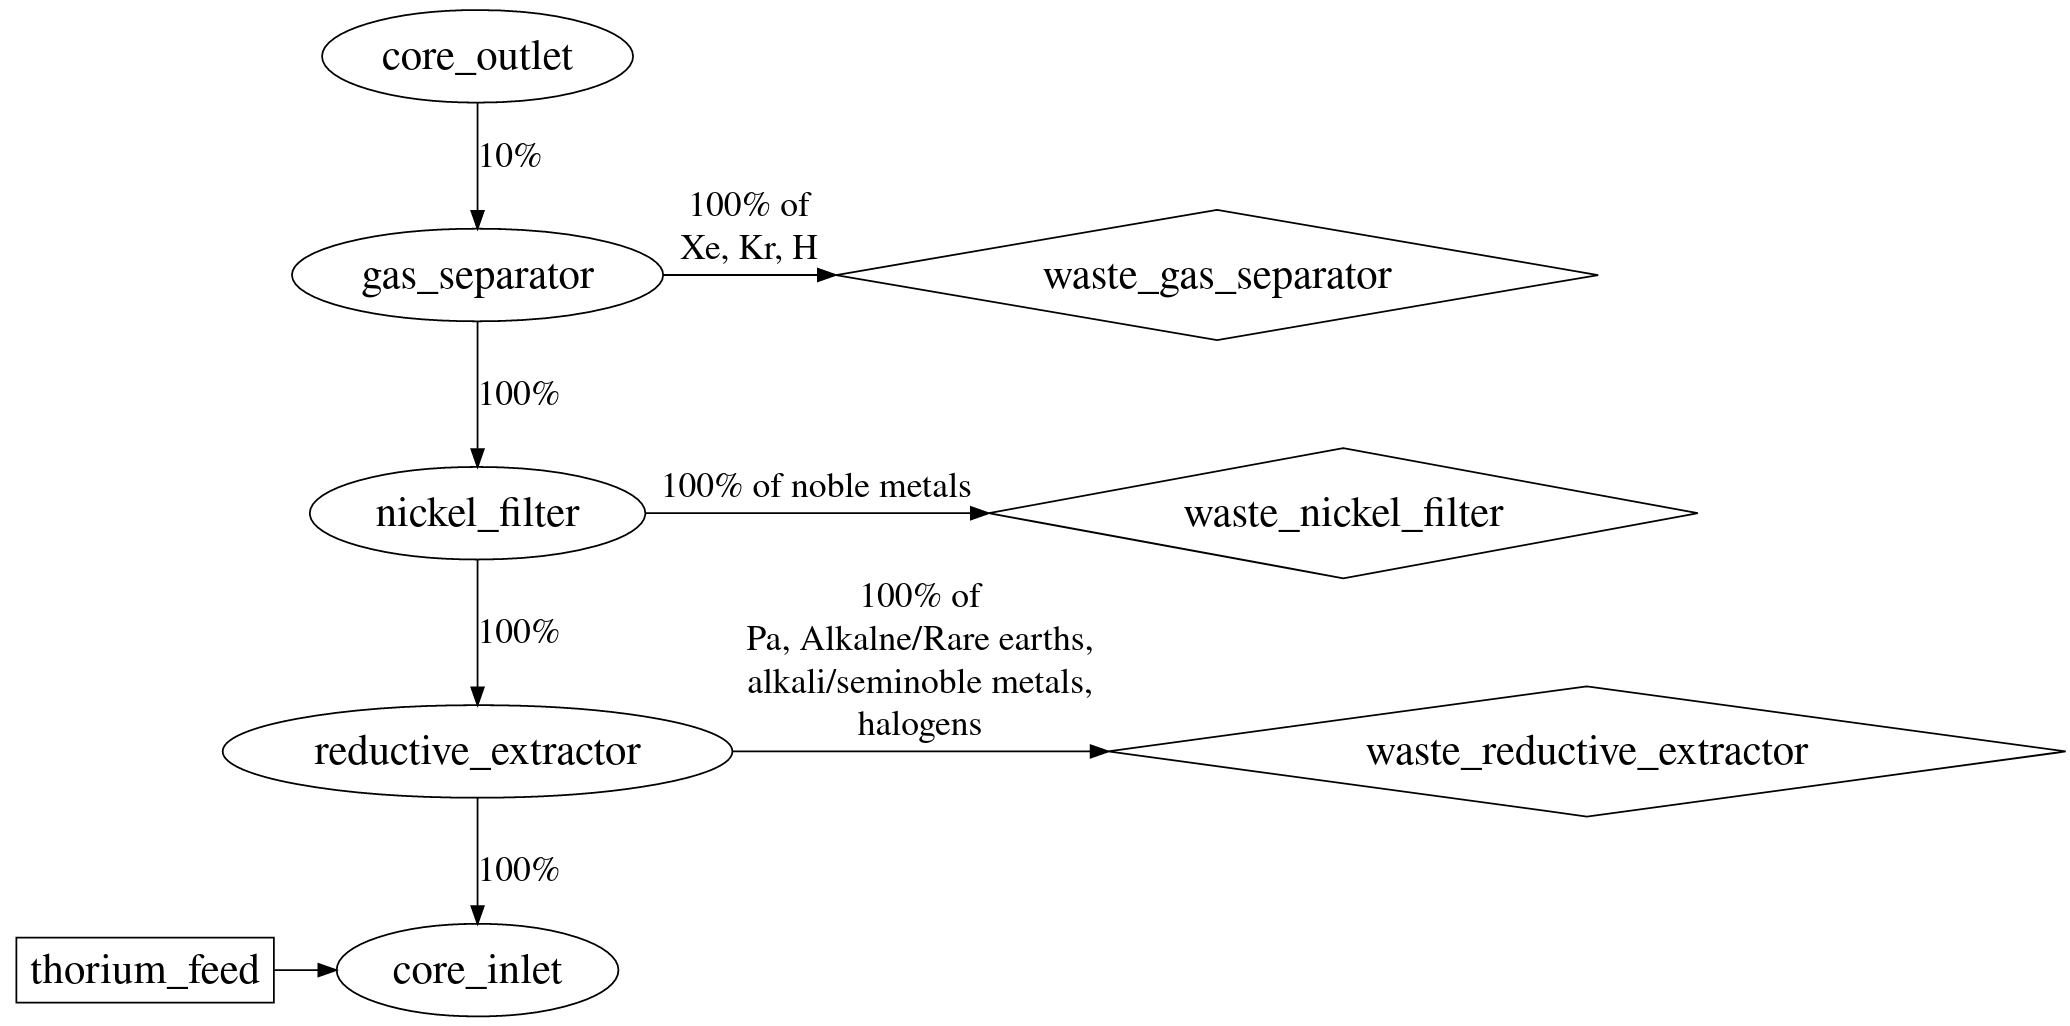
\includegraphics[width=0.8\textwidth]{figs/ch4/process_graph.png}
    \caption{Process graph for model salt reprocessing system}
    \label{fig:process-graph}
\end{figure}

Table \ref{tab:msbr-cycle-times} lists element groups and their extraction
efficiencies. Note the presence of a \verb.thorium_feed. feed process. This
process replaces the lost mass via reprocessing with an equal mass of fuel salt
of identical composition to the initial fuel salt, but with all \ce{^{233}U}
replaced by \ce{^{232}Th}. This ensures we have a relatively constant level of
\ce{^{232}Th} in the reactor.

\begin{table}[htpb] 
    \centering 
    \caption{Extraction efficiencies using cycle times in Table \ref{tab:msbr-cycle-times} and Equation \ref{eq:extraction-efficiency}}
    \label{tab:msbr-cycle-times}
    \begin{tabularx}{400pt}{|X|X|X|X|X|} 
        \hline
        Processing group & Target component(s) & Cycle time for processing & Processing component & Extraction efficiency\\
        \hline
        Protactinium & \ce{^{233}Pa} & 3 days & reductive extractor & 1\\
        \hline
        Rare earths & Trivalent: \ce{Y}, \ce{La}, \ce{Ce}, \ce{Pr}, \ce{Nd}, \ce{Pm}, \ce{Gd}, Divalent: \ce{Sm}, \ce{Eu} & 50 days (500 for \ce{Eu}) & reductive extractor & 0.8904 (0.2 for \ce{Eu})\\
        \hline 
        Noble metals & \ce{Se}, \ce{Nb}, \ce{Mo}, \ce{Tc}, \ce{Ru}, \ce{Rh}, \ce{Pd}, \ce{Ag}, \ce{Sb}, \ce{Te} & 20 sec & nickel filter & 1\\
        \hline
        Seminoble metals & \ce{Zr}, \ce{Cd}, \ce{In}, \ce{Sn} & 200 days & reductive extractor & 0.425\\
        \hline
        Gases & \ce{Kr}, \ce{Xe} & 20 sec & gas separator & 1\\
        \hline
        Halogens & \ce{Br}, \ce{I} & 60 days & reductive extractor & 0.842\\
        \hline
        Alkaline earths; alkali metals & \ce{Sr}, \ce{Ba}; \ce{Rb}, \ce{Cs} & 3435 days & reductive extractor & 0.032 \\
        \hline
    \end{tabularx}
\end{table}

\section{Cross Section Data}
\label{sec:xs-data}
Ryklevskii used the JEFF 3.1.2 cross section library in the initial evaluation of the \Gls{msbr} CSG model. I have not been able to convert the JEFF 3.1.2 library to \OpenMC's HDF5 format, so I am instead using the ENDF/B VII.1 cross section library.

\section{Differences between the \OpenMC and \SerpentTWO models}
The only differences between the \OpenMC and \SerpentTWO CSG models are in the
construction of the geometry. The \OpenMC model is constructed programmatically
using the OpenMC Python API, whereas the \SerpentTWO model is written entirely
in an input file. I encourage interested readers to compare the files stored at
\url{github.com/arfc/2022-yardasol-ms/tree/model/} under \verb.openmc/. and
\verb.serpent/.

%\chapter{Results}
\label{ch:chapter5}

\subsection{Platform and Software}
\label{sub:platform-software}
I ran the \OpenMC simulation on Sawtooth, a supercomputer at \Gls{inl}.
I previously attempted to use Theta, a supercomputer at \Gls{anl}, for this
simualation, however \OpenMC
Use of export controlled code is currently prohibited on Theta, so for our \SerpentTWO runs,
we used a Dell Precision 3430 Workstation.

% make this subsection a table
% Talk about KNL, cross compiling, etc\ldots
Theta's compute nodes and constancia nodes used cross-compilation\ldots

\begin{table}[htpb] 
    \centering 
    \caption{Theta job parameters for 100k particle \OpenMC run}
    \label{tab:theta-params}
    \begin{tabular}{|c|c|c|} 
        \hline
        Quantity & \verb.aprun. option & Value\\
        \hline
        Nodes & \verb.-n. & 128 \\
        \hline
        MPI processes per node & \verb.-N. 4 \\
        \hline
        Threads per core & \verb.-j. & 4 \\
        \hline
        MPI Process binding & \verb.-cc. & depth \\
        \hline
        Depth & \verb.-d. & ?? \\
        \hline
        OpenMP threads per MPI process & \verb.-e OMP_NUM_THREADS=64. & 64 \\
        \hline
        Clustering mode & -- & SNC-4 \\
        \hline
        Memory mode & -- & Cache \\
        \hline
    \end{tabular}
\end{table}
% make this subsection a table

\subsection{Simulation Design and Parameters}
\label{sub:simulation-parameters}

I design


Table \ref{tab:saltproc-params} summarizes the simulation settings used
for both the \SerpentTWO and \OpenMC simulations.
 
\begin{table}[htpb] 
    \centering 
    \caption{Neutronics and Depletion parameters for SaltProc}
    \label{tab:saltproc-params}
    \begin{tabular}{|c|c|} 
        \hline
        Batches & 200 \\
        \hline
        Inactive batches & 80 \\
        \hline
        Particles per batch & 1e6 \\
        \hline
        Power [W] & 2.25e9 \\
        \hline
        Depletion steps & 122 \\
        \hline
        Depletion step length [days] & 3 \\
        \hline
        Depletion equation solver & IPF CRAM 48 \\
        \hline
        Time integration method & Euler's Method \\
        \hline
    \end{tabular}
\end{table}

\subsection{Data}
\label{sub:results-xs-data}

I used the ENDF/B-VII.1 library for both the \SerpentTWO and
\OpenMC simulations (cite endfb). I specifically used the neutron reaction,
neutron induced fission product yields, and spontaneous fission product yields
sublibraries. I used the thermal neutron scattering sublibrary from the
ENDF/B-VII.0 library, which contains the same data as what is in the
ENDF/B-VII.1 library. The thermal neutron scattering sublibray in ENDF/B-VII.1
uses a continuous representation that \SerpentTWO v2.1.32 does not support.

To ensure data consistency, I donwloaded the \verb,.ace, files from the NNDC
website, then processed these files into HDF5 format using the \OpenMC Python
API. I also used the Python API to create a depletion chain from the
spontaneous and delayed fission yield data, decay data, and neutron cross
secttion data from the ENDF B/VII.1 library. Interested readers are able to
create this library files by running the scripts located at
\url{https://github.com/arfc/saltproc/tree/master/scripts/xsdata}.\footnote{See
the \verb,README.md, in the parent directory for user instructions}.

We assumed material temperatures to be around 900K. For cross section data
unavailable at that temperature, we used interpolation between 800K and 1000
to get reasonable values.
 

\section{Comparison of OpenMC to Serpent}
\label{sec:openmc-vs-serpent}


%\input{chatper6_conclusions}

\appendix
\appendix
\chapter*{Appendix B: SaltProc input file structure}
\label{appex:input-files}
\definecolor{bg}{rgb}{0.95,0.95,0.95}

\begin{listing}[!ht]
    \begin{minted}[frame=single,
                   framesep=3mm,
                   tabsize=4,
                   bgcolor=bg,
                   fontsize=\footnotesize]{json}
    {
      "Path to Serpent executable": "sss2",
      "File containing processing system objects": "msbr_objects.json",
      "Graph file containing processing system structure": "msbr.dot",
      "User's Serpent input file with reactor model": "msbr.serpent",
      "Path output data storing folder": "../../saltproc/data/",
      "Output HDF5 database file name": "msbr_kl_100_saltproc.h5",
      "Number of neutrons per generation": 50,
      "Number of active generations": 20,
      "Number of inactive generations": 20,
      "Restart simulation from the step when it stopped?": false,
      "Geometry file/files to use in Serpent runs": "geometry/msbr_full.ini",
      "Switch to another geometry when keff drops below 1?": false,
      "Salt mass flow rate throughout reactor core (g/s)": 9920000,
      "Number of steps for constant power and depletion interval case": 12,
      "Depletion step interval or Cumulative time (end of step) (d)": 3,
      "Reactor power or power step list during depletion step (W)": 2250000000
    }
    \end{minted}
    \caption{\SaltProc v0.3.0 input file}
    \label{listing:1}
\end{listing}

\begin{listing}[!ht]
    \begin{minted}[frame=single,
                   framesep=3mm,
                   tabsize=4,
                   bgcolor=bg,
                   fontsize=\footnotesize]{json}
    {
       "proc_input_file": "msbr_objects.json",
       "dot_input_file": "msbr.dot",
       "output_path": "./data",
       "num_depsteps": 12,
       "depcode": {
           "codename": "serpent",
           "exec_path": "sss2",
           "template_inputfile_path": "./msbr.serpent",
           "iter_inputfile": "saltproc_serpent",
           "iter_matfile": "saltproc_mat",
           "npop": 50,
           "active_cycles": 20,
           "inactive_cycles": 20,
           "geo_file_paths": ["./geometry/msbr_full.ini"]
       },
       "simulation": {
           "sim_name": "msbr_example_simulation",
           "db_name": "msbr_kl_100_saltproc.h5",
           "restart_flag": false,
           "adjust_geo": false
       },
       "reactor": {
           "volume": 1.0,
           "mass_flowrate": 9920000,
           "power_levels": [ 2250000000 ],
           "dep_step_length_cumulative": [ 3 ]
       }
    }
    \end{minted}
    \caption{\SaltProc v0.4.0 input file}
    \label{listing:2}
\end{listing}

\begin{listing}[!ht]
    \begin{minted}[frame=single,
                   framesep=3mm,
                   tabsize=4,
                   bgcolor=bg,
                   fontsize=\footnotesize]{json}
    {
       "proc_input_file": "msbr_objects.json",
       "dot_input_file": "msbr.dot",
       "n_depletion_steps": 12,
       "depcode": {
           "codename": "serpent",
           "template_input_file_path": "msbr.serpent",
           "geo_file_paths": ["geometry/msbr_full.ini"]
       },
       "simulation": {
           "sim_name": "msbr_kl_100_simulation"
       },
       "reactor": {
           "volume": 1.0,
           "mass_flowrate": 9920000,
           "power_levels": [ 2250000000 ],
           "depletion_timesteps": [ 3 ],
           "timestep_units": "d"
       }
    }
    \end{minted}
    \caption{\SaltProc v0.5.0 input file}
    \label{listing:3}
\end{listing}




\backmatter

\bibliographystyle{apalike}
\bibliography{bibliography}

\end{document}
\endinput
%%
%% End of file `thesis-ex.tex'.
